\chapter{Resultados}

\section{Levantamiento de información}
Por medio del levantamiento de información es posible hacer un pequeño análisis del estado actual y los datos obtenidos. Por un lado, la estructura actual responde a la necesidad de colocar la máquina en una ubicación transitoria, debido a los trabajos realizados en el piso del laboratorio durante el año 2012. Por lo mismo, no está diseñada para la operación de la máquina bajo ningún contexto por los peligros que conlleva. Aún cuando esta podría ser modificada, se desconocen las características y propiedades de la especie maderera con la que fue fabricada, lo que obliga a diseñar y construir un nuevo soporte para la máquina. 

Por otra parte, la información obtenida de la máquina de fatiga da cuenta de tres puntos importantes. La antigüedad de sus componentes y la tecnología utilizada afecta directamente en su mantenimiento ante la dificultad de encontrar piezas de repuesto, debido a que las dimensiones de sus componentes, como la polea y la correa, se encuentran fuera de catálogo o de las dimensiones de fabricación de los proveedores. También la obsolescencia de la tecnología tienen incidencia, siendo difícil poder encontrar no sólo las piezas de repuesto, sino que también personas que estén técnicamente calificadas. En segundo lugar, la máquina fue fabricada con estándares o líneas de desarrollo propias de la época, como sería esperable, las cuales no evolucionaron en la misma dirección que los estándares actuales de ensayo a fatiga, dificultando la comparación de los resultados obtenidos. Finalmente, la robustez del diseño, la cual se puede apreciar fácilmente en la dimensiones de la estructura exterior de la máquina, tiene la dualidad de proveer un armazón macizo y duradero sobre el cual trabajar, por el contrario, resulta ser una estructura difícil de modificar por esta misma razón.

En lo relativo a la exactitud de los datos obtenidos, la imposibilidad de desarmar gran parte de la máquina afectaron la precisión de las mediciones realizadas, sobre todo en partes específicas. Así, las dimensiones y la geometría de las vigas en voladizo tuvieron que ser simplificadas ante la imposibilidad de tomar medidas en la unión barra-disco. Por la misma razón, la masa del disco desbalanceado, calculada a través de la deflexión de las vigas de acero en voladizo, incluye los errores de la medición anterior sumado a la masa de otros elemento que no son parte de la fuerza provocada por el desequilibrio del disco en rotación. Ante esto, surge la necesidad de poder desarmar la máquina para poder estudiarla con mayor detenimiento, obteniendo información que sea más precisa de sus elementos como también información útil para poder actualizar componentes que mejoren su desempeño y mantenibilidad. 
 
\section{Diseño de la estructura}
\subsection{Diseño de pletinas de acero}
A partir de las ec. \ref{eq:reaccion_acero}, \ref{eq:mtofleca_acero} y \ref{eq:esfmax_acero}, expuestas en la sección de diseño en acero en metodología, se probó de forma iterativa para distintas dimensiones del acero A270ES, su comportamiento bajo la carga estática. Como se señaló anteriormente, sólo se tomó en consideración pletinas de un ancho de 100 mm debido al espaciamiento necesario entre los pernos. Los resultados que se obtuvieron se encuentran en la siguiente tabla \ref{tab:itest_acero}.

\begin{table}[h]
\centering
\resizebox{\textwidth}{!}{%
\begin{tabular}{@{}ccccccc@{}}
\toprule
N$^{\circ}$ & Dimensiones {[}mm{]} & $\bar{I}$ {[}mm$^4${]} & $R_A$ {[}N{]} & $M_A$ {[}Nm{]} & $\sigma_{max,pl}$ {[}MPa{]} & Factor de Seguridad {[}-{]} \\ \midrule
1 & 100x10 & 8333,33 & 23,87 & 2,46 & 60,88 & 4,43 \\
2 & 100x6 & 1800 & 14,32 & 1,48 & 167,46 & 1,61 \\
3 & 100x5 & 1041,66 & 11,95 & 1,23 & 240,56 & 1,12 \\
4 & 100x8 & 4266,66 & 19,09 & 1,97 & 94,66 & 2,85 \\ \bottomrule
\end{tabular}%
}
\caption{Resultados y factor de seguridad para distintas configuraciones de pletinas de acero.}
\label{tab:itest_acero}
\end{table}

Con esta información en consideración, se comprobará su comportamiento bajo las cargas dinámicas, descartando el acero número 1 por estar sobredimensionado. Utilizando la ecuación \ref{eq:mtofat_pletacero} se obtiene que el momento provocado por la carga alternante es $M_{a,pl,A} =$ 33,64 [Nm]. Esta fuerza alternante corresponde a la carga alcanzada por la máquina de fatiga al llegar al esfuerzo último de la probeta. De esta manera, al aplicar las ecuaciones \ref{eq:esffat_pletacero} y \ref{eq:fs_fatacero} se obtienen los resultados que se encuentran en la tabla \ref{tab:itfat_acero}

\begin{table}[h]
\centering
\begin{tabular}{@{}cccc@{}}
\toprule
N$^{\circ}$ & Dimensiones [mm] & $\sigma_{a,A}$ [MPa] & Factor de Seguridad [-] \\ \midrule
2 & 100x6 & 56,06 & 1,50 \\
3 & 100x5 & 80,73 & 1,04 \\
4 & 100x8 & 31,53 & 2,66 \\ \bottomrule
\end{tabular}
\caption{Resultados de esfuerzo alternante y factor de seguridad a fatiga para distintas configuraciones de pletinas de acero.}
\label{tab:itfat_acero}
\end{table}

Con esto, el factor de seguridad del acero N$^{\circ}$ 3 resulta cercano a 1, lo cual nos indica que sus esfuerzos están en la recta de Goodman. Por lo tanto, se trabajará a partir de las dimensiones del acero N$^{\circ}$ 4, por otorgar un factor de seguridad que no se encuentre demasiado cerca de la recta de Goodman como lo es en el caso del acero N$^{\circ}$ 2. 

\subsection{Diseño en madera}
Para este caso, los resultados se dividirán por cada uno de los componentes que se calcularon en la estructura. Se expondrán, a modo de comparación, los cálculos realizados para dos formatos distintos de pino oregón, tanto para los elementos A y B como el elemento C.

\subsubsection{Viga A} Los cálculos de reacción y momento flector máximo se obtiene a través de las ecuaciones \ref{eq:reac_vigappal} y \ref{eq:mto_vigappal}. Así, los resultados obtenidos para la sección flexo-comprimida, flexo-traccionada y los esfuerzos cortantes son:
\begin{table}[h]
\centering
\resizebox{\textwidth}{!}{%
\begin{tabular}{ccccccccc}
\hline
N$^{\circ}$ & Dimensiones [mm] & $R_o$ [N] & $M_o$ [Nm] & $f_f$ [MPa] & $F_{ft,dis}$ [MPa] & $F_{fv,dis}$ [MPa] & $f_{cz}$ [MPa] & $F_{cz}$ [MPa] \\ \hline
1 & 110x110 & 795,02 & 122,26 & 0,551 & 7,08 & 7,74 & 0,77 & 0,09 \\
2 & 85x85 & 781,24 & 119,57 & 1,168 & 7,29 & 7,73 & 0,16 & 0,77 \\ \hline
\end{tabular}%
}
\caption{Resultados obtenidos para la flexión y cizalle de la viga A.}
\label{tab:res_viga_a1}
\end{table}
\\
En base a estos resultados, el factor de seguridad de cada formato es:

\begin{table}[H]
\centering
\begin{tabular}{@{}ccccl@{}}
\toprule
N$^{\circ}$ & Dimensiones [mm] & $FS_{ft}$ & $FS_{fv}$ & $FS_{cz}$ \\ \midrule
1 & 110x110 & 12,85 & 14,03 & 7,84 \\
2 & 85x85 & 6,24 & 6,62 & 4,77 \\ \bottomrule
\end{tabular}
\caption{Factores de seguridad en la viga A.}
\label{tab:res_viga_a2}
\end{table}

\subsubsection{Pilar B}
Esta viga se encuentra en compresión paralela a la fibra, al soportar toda la carga y transmitirla hacia el piso. En la tabla \ref{tab:res_viga_b}, se actualizaron los cálculos realizados en la sección de metodología al incorporar el área neta de cada formato de madera, es decir, el área transversal menos el área de cada unión, en este caso, del perno de 0,5 pulgadas de diámetro que une el pilar B a la viga D.

\begin{table}[h]
\centering
\begin{tabular}{@{}ccccccc@{}}
\toprule
N$^{\circ}$ & Dimensiones [mm] & $\lambda$ & $f_{cp}$ [MPa] & $F_{cp,dis}$ [MPa] & $F_{cp,\lambda,dis}$ [MPa] & $FS_{cp,\lambda}$ \\ \midrule
1 & 110x110 & 37,32 & 0,0742 & 5,936 & 4,506 & 66,6 \\
2 & 85x85 & 49,82 & 0,129 & 5,936 & 3,872 & 28,9 \\ \bottomrule
\end{tabular}
\caption{Esfuerzos y factor de seguridad por compresión paralela en la viga B.}
\label{tab:res_viga_b}
\end{table}

\subsubsection{Viga C}
Como se señaló en metodología, la viga C no recibe mayores cargas, por lo tanto los criterios de selección se fundamentan en la longitud necesaria de los tirafondos para lograr penetrar la viga A sin que el roscado toque la viga C. La tabla de cálculos para dos configuraciones de tablas distintas son:

\begin{table}[h]
\centering
\begin{tabular}{@{}cclccc@{}}
\toprule
N$^{\circ}$ & Dimensiones & Estado & $\bar{I}$ [mm$^4$] & $f_f$ [kPa] & $F_f$ [MPa] \\ \midrule
1 & 1x8'' & Cepillada & 1,0$\cdot 10^7$ & 3,804 & 3,925 \\
2 & 2x8'' & Cepillada & 2,16$\cdot 10^7$ & 1,763 & 3,925 \\ \bottomrule
\end{tabular}
\caption{Segundo momento de área y esfuerzos de carga y diseño en la viga C.}
\label{tab:res_viga_c}
\end{table}

\subsubsection{Selección de formatos}
Como se aprecia, todos los elementos se encuentran sobredimensionados respecto a las solicitaciones requeridas. En el caso de los elementos A y B, el factor de seguridad más bajo corresponde al cizalle de la viga A. Si bien el factor de seguridad en el formato n$^{\circ}$ 1 es casi el doble al formato n$^{\circ}$ 2, se optará por el primero por el amortiguamiento de las vibraciones de la máquina que otorga la madera.

Por otro lado, en la viga C las cargas son menores y, por lo tanto, su elección se debe al de espesor mínimo para que el tirafondo sea capaz de penetrar la viga A. Al ser 1'' el espesor mínimo existente en el mercado, se optó por el formato n$^{\circ}$ 1.

Por lo tanto, los formatos a utilizar en el diseño corresponden a 110x110 mm para los elementos A y B y de 1x8'' para el elemento C.

\subsection{Uniones mecánicas}

Como se señaló en la metodología, los cálculos correspondiente a uniones mecánicas se limita a los pernos de unión entre las pletinas y la viga A y a los tirafondos que unen la viga C con A y B.

\subsubsection{Pernos}
Para este elemento de unión, el largo utilizado se fijó en 5,5 pulgadas para que sea capaz de atravesar todos los elementos a unir y los diámetros a probar dependieron de su disponibilidad en el mercado. Los resultados se muestran en la tabla \ref{tab:res_perno}. 

Al seleccionar el perno número 1, la tabla \ref{tab:res_seppernos} muestra las restricciones de separación en base a su diámetro.

\begin{table}[h]
\centering
\resizebox{\textwidth}{!}{%
\begin{tabular}{@{}cccccccc@{}}
\toprule
$N^{\circ}$ & Diámetro [in] & $\lambda_u$ & $F_{ap}$ [MPa] & $P_{ad,simple}$ [MPa] & $Z\cdot D^2$ & \begin{tabular}[c]{@{}c@{}}Cumple \\ $F_{ap} \lambda_u D^2\leq Z\cdot D^2$\end{tabular} & $FS_{perno}$ \\ \midrule
1 & $1/4$ & 2,52 & 3,52 & 178,89 & 964,01 & Sí & 3,76 \\
2 & $5/16$ & 2,02 & 3,46 & 219,82 & 1493,44 & Sí & 7,23 \\
3 & $3/8$ & 1,68 & 3,40 & 259,24 & 2131,94 & Sí & 12,28 \\ \bottomrule
\end{tabular}%
}
\caption{Cargas admisibles y factor de seguridad para distintos pernos hexagonales.}
\label{tab:res_perno}
\end{table}

\begin{table}[h]
\centering
\begin{tabular}{@{}cccc@{}}
\toprule
Diámetro [in] & $S_{bcn}$ [mm] & $S_{bdn}$ [mm] & $S_p$ [mm] \\ \midrule
$1/4$ & 25,4 & 12,7 & 44,45 \\ \bottomrule
\end{tabular}
\caption{Separación del perno a borde cargado, descargado y entre pernos, a partir de su diámetro.}
\label{tab:res_seppernos}
\end{table}

\subsubsection{Tirafondos}

En el caso de los tirafondos, se fijará un diámetro de \nicefrac{1 }{ 4}'' para poder estar dentro de los espaciamientos recomendados por la norma, mostrados en la tabla \ref{tab:res_septirafondo}. 

\begin{table}[h]
\centering
\begin{tabular}{@{}cccc@{}}
\toprule
Diámetro [in] & $S_{bcn}$ [mm] & $S_{bdn}$ [mm] & $S_p$ [mm] \\ \midrule
$1/4$ & 25,6 & 12,8 & 44,8 \\ \bottomrule
\end{tabular}
\caption{Espaciamiento entre los bordes cargado, descargado y entre tirafondos, para un diámetro de 1/4 de pulgada.}
\label{tab:res_septirafondo}
\end{table}

Se calcularon distintas longitudes de tirafondos existentes en el mercado para seleccionar el indicado. Así, la tabla \ref{tab:res_tirafondos} muestra que para los 3 largos distintos se cumplen con los requisitos de penetración \footnote{La definición de la profundidad mínima de penetración y la penetración mínima del vástago se encuentran en el anexo \ref{sec:tirafondos}}, los esfuerzos admisibles y el factor de seguridad.

\begin{table}[h]
\centering
\resizebox{\textwidth}{!}{%
\begin{tabular}{@{}ccccccc@{}}
\toprule
N$^{\circ}$ & Largo [in] & \begin{tabular}[c]{@{}c@{}}Profundidad mínima\\ de penetración\end{tabular} & \begin{tabular}[c]{@{}c@{}}Penetración mínima del\\ vástago en pieza central\end{tabular} & \begin{tabular}[c]{@{}c@{}}Esfuerzo admisible de\\ extracción lateral total \\ $P_{el,ad,total}$ [kN]\end{tabular} & \begin{tabular}[c]{@{}c@{}}Esfuerzo admisible de\\ extracción directa total \\ $P_{ed,ad,total}$ [kN]\end{tabular} & $FS_{tirafondo}$ \\ \midrule
1 & 1 $1/2$ & Cumple & Cumple & 1245,07 & 5,53 & 1,38 \\
2 & 2 & Cumple & Cumple & 1348,82 & 10,9 & 2,72 \\
3 & 2 $1/2$ & Cumple & Cumple & 1452,58 & 15,52 & 3,87 \\ \bottomrule
\end{tabular}%
}
\caption{Esfuerzos admisibles y factor de seguridad para distintas longitudes de tirafondo.}
\label{tab:res_tirafondos}
\end{table}

Por lo tanto, se seleccionó el tirafondo de n$^{\circ}$ 1, para no sobredimensionar los elementos de unión. La selección de este formato es distinta a la expuesta en la sección de metodología, sin embargo, ambos cumplen con los requisitos expuestos. 

%\newpage

\subsection{Simulación estática y modal}

Al seleccionar y definir cada elemento de la estructura, se realizaron las simulaciones estática y modal de la misma. De la simulación modal, los seis primeros valores de la frecuencia natural de la estructura se ven en la tabla \ref{tab:frec_nat}, de las cuales todas se encuentran por sobre el rango de vibración de la máquina de fatiga y su motor. Además, en las figuras \ref{fig:frecuencias_mesa} se muestra el movimiento de la estructura para cada frecuencia.

\begin{table}[h]
\centering
\begin{tabular}{@{}cccccccc@{}}
\toprule
N$^{\circ}$ &  $\omega_{motor}$ & F1 & F2 & F3 & F4 & F5 & F6  \\ \midrule
Frecuencia [Hz] & 25 & 128,43 & 135,24 & 143,48 & 145,79 & 175,23 & 189,92 \\ \bottomrule
\end{tabular} 
\caption{Valores de la frecuencia natural de la estructura obtenidos por medio del análisis modal del software Inventor. }
\label{tab:frec_nat}
\end{table}

\begin{figure}[]
\centering
	\begin{subfigure}{0.5\linewidth}
		\centering
		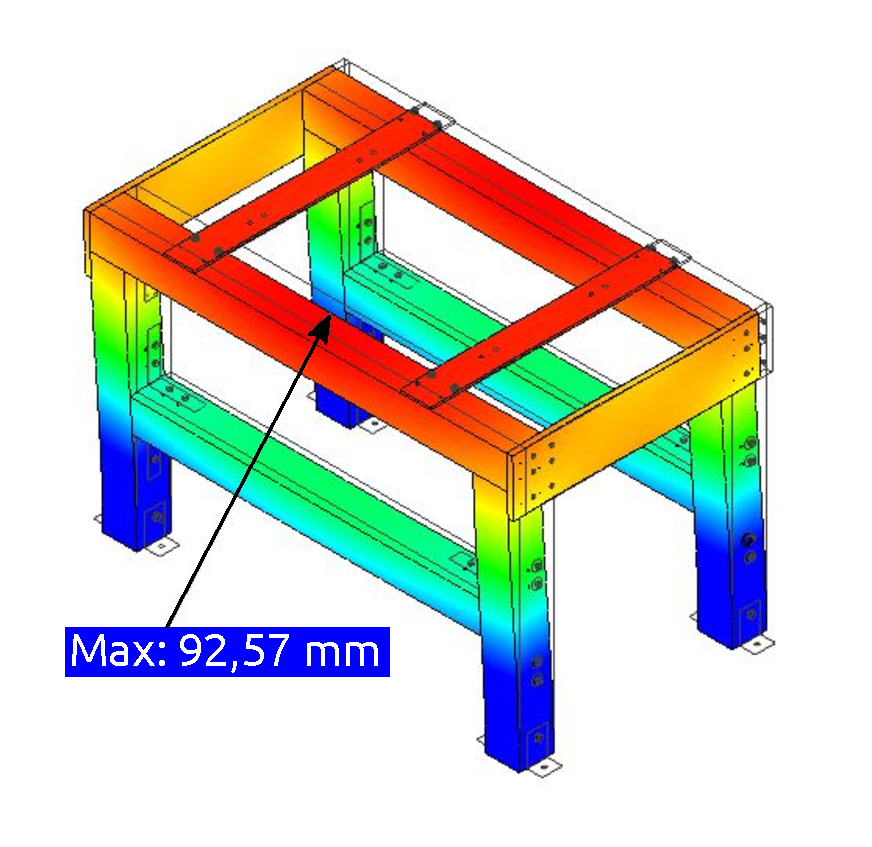
\includegraphics[width=0.9\linewidth]{Imagenes/F1.pdf}
		\caption{$f_1 = 128.43$ Hz}\label{fig:frecuencia_1}
	\end{subfigure}%
	\begin{subfigure}{0.5\linewidth}
		\centering
		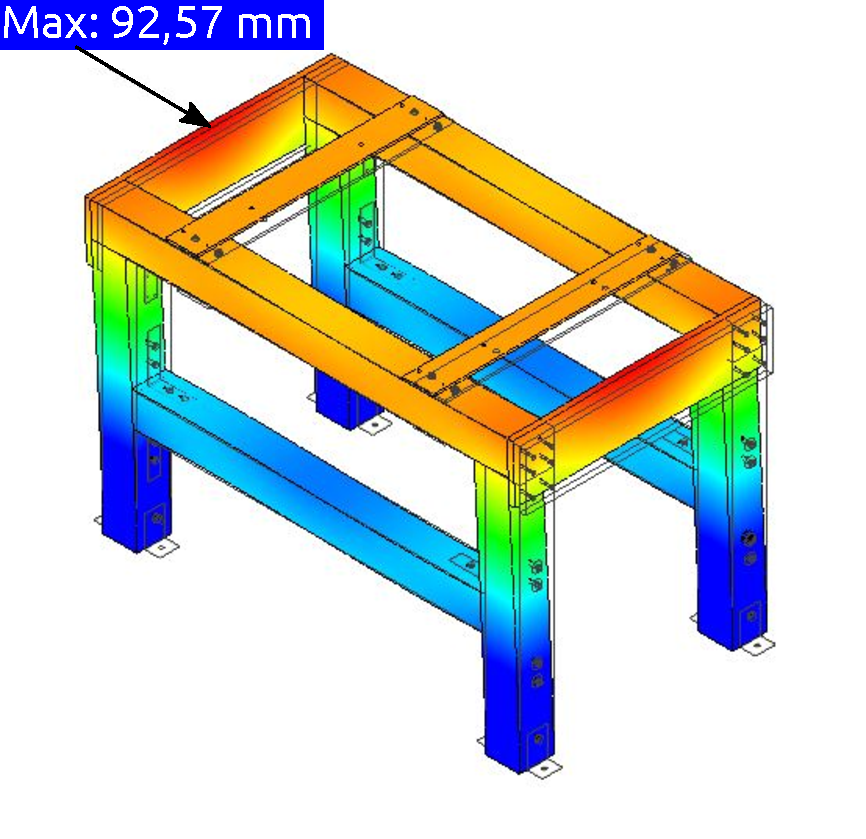
\includegraphics[width=0.9\linewidth]{Imagenes/F2.pdf}
		\caption{$f_2 = 135.24$ Hz}\label{fig:frecuencia_2}
	\end{subfigure}
		\begin{subfigure}{0.5\linewidth}
		\centering
		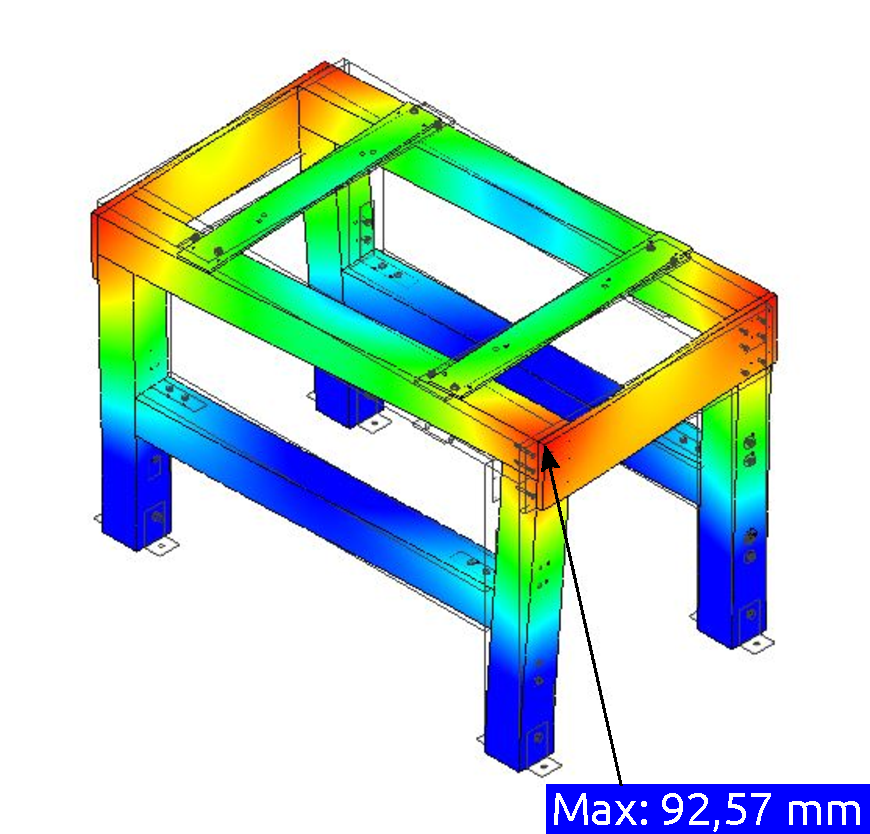
\includegraphics[width=0.9\linewidth]{Imagenes/F3.pdf}
		\caption{$f_3 = 143.48$ Hz}\label{fig:frecuencia_3}
	\end{subfigure}%
	\begin{subfigure}{0.5\linewidth}
		\centering
		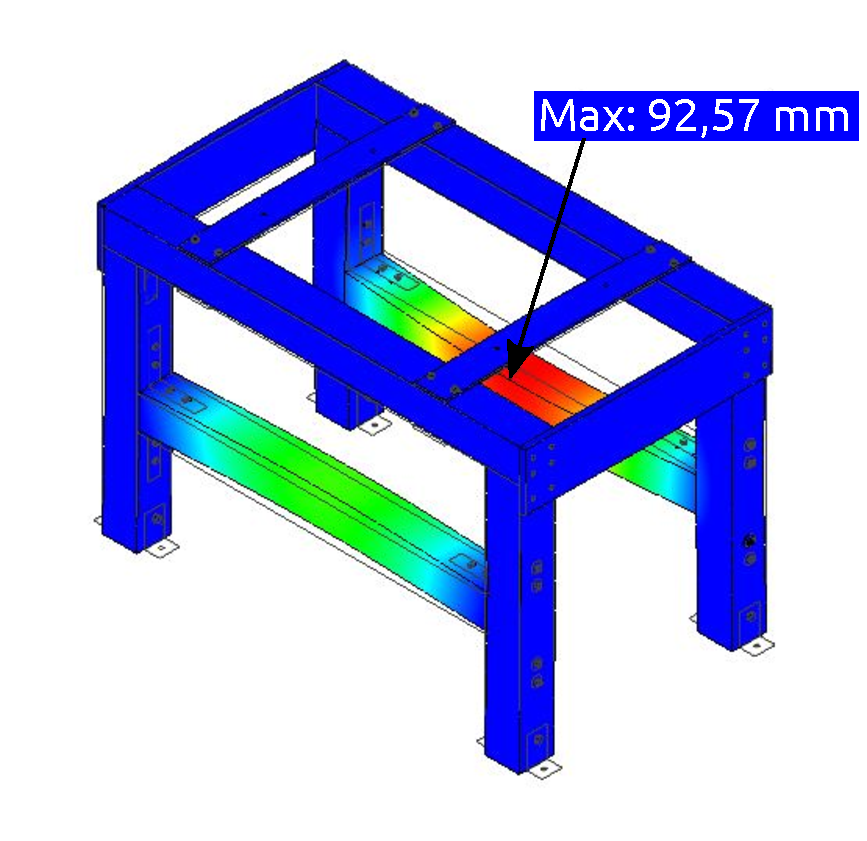
\includegraphics[width=0.9\linewidth]{Imagenes/F4.pdf}
		\caption{$f_4 = 145.79$ Hz}\label{fig:frecuencia_4}
	\end{subfigure}
		\begin{subfigure}{0.5\linewidth}
		\centering
		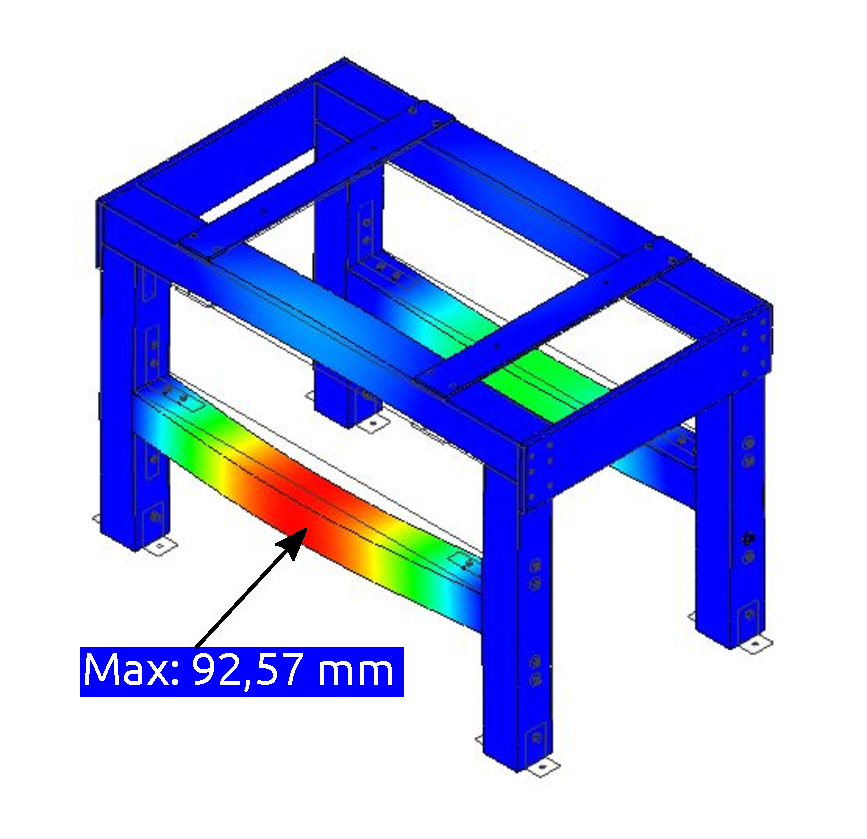
\includegraphics[width=0.9\linewidth]{Imagenes/F5.pdf}
		\caption{$f_5 = 175.23$ Hz}\label{fig:frecuencia_5}
	\end{subfigure}%
	\begin{subfigure}{0.5\linewidth}
		\centering
		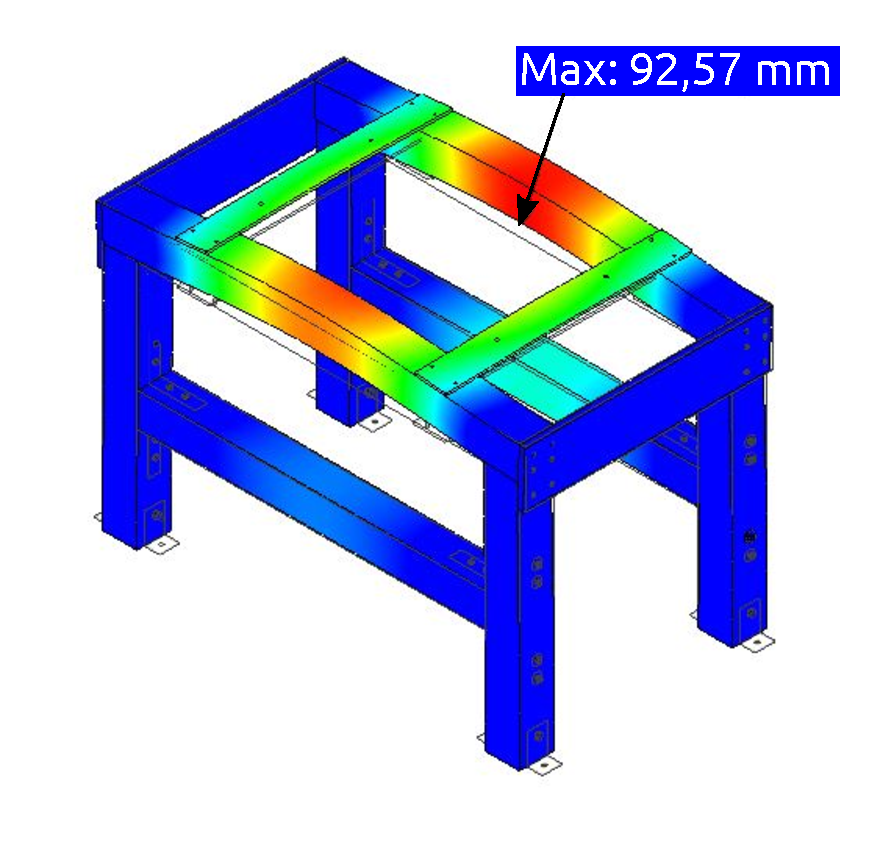
\includegraphics[width=0.9\linewidth]{Imagenes/F6.pdf}
		\caption{$f_6 = 189.92$ Hz}\label{fig:frecuencia_6}
	\end{subfigure}
\caption{Modos de vibración de las seis primeras frecuencias naturales de la estructura soportante.}
\label{fig:frecuencias_mesa}
\end{figure}

Del análisis estático, se pudo comprobar que las zonas críticas del diseño se encuentran en el acero, como se puede apreciar en la fig. \ref{fig:resultados_mesa}. Esto confirma el trabajo de cálculo, expuesto anteriormente, el cual establece que el esfuerzo máximo se encuentra en el empotramiento de la pletina de acero, es decir, en el punto $A$ utilizando como referencia el diagrama de cargas \ref{fig:diagcargas_viga_acero}. Si bien los valores de los esfuerzos son mayores en los cálculos que en la simulación, se debe tener en cuenta que en la simulación se utilizó una carga distribuida aplicada sobre la máquina de fatiga. Además, fueron los cálculos los que se utilizaron para justificar las dimensiones del diseño, lo cual frente a esta diferencia de resultados, se resume en un posible sobredimensionamiento de la pletina de acero.

\begin{figure}[h]
\centering
	\begin{subfigure}{0.49\linewidth}
		\centering
		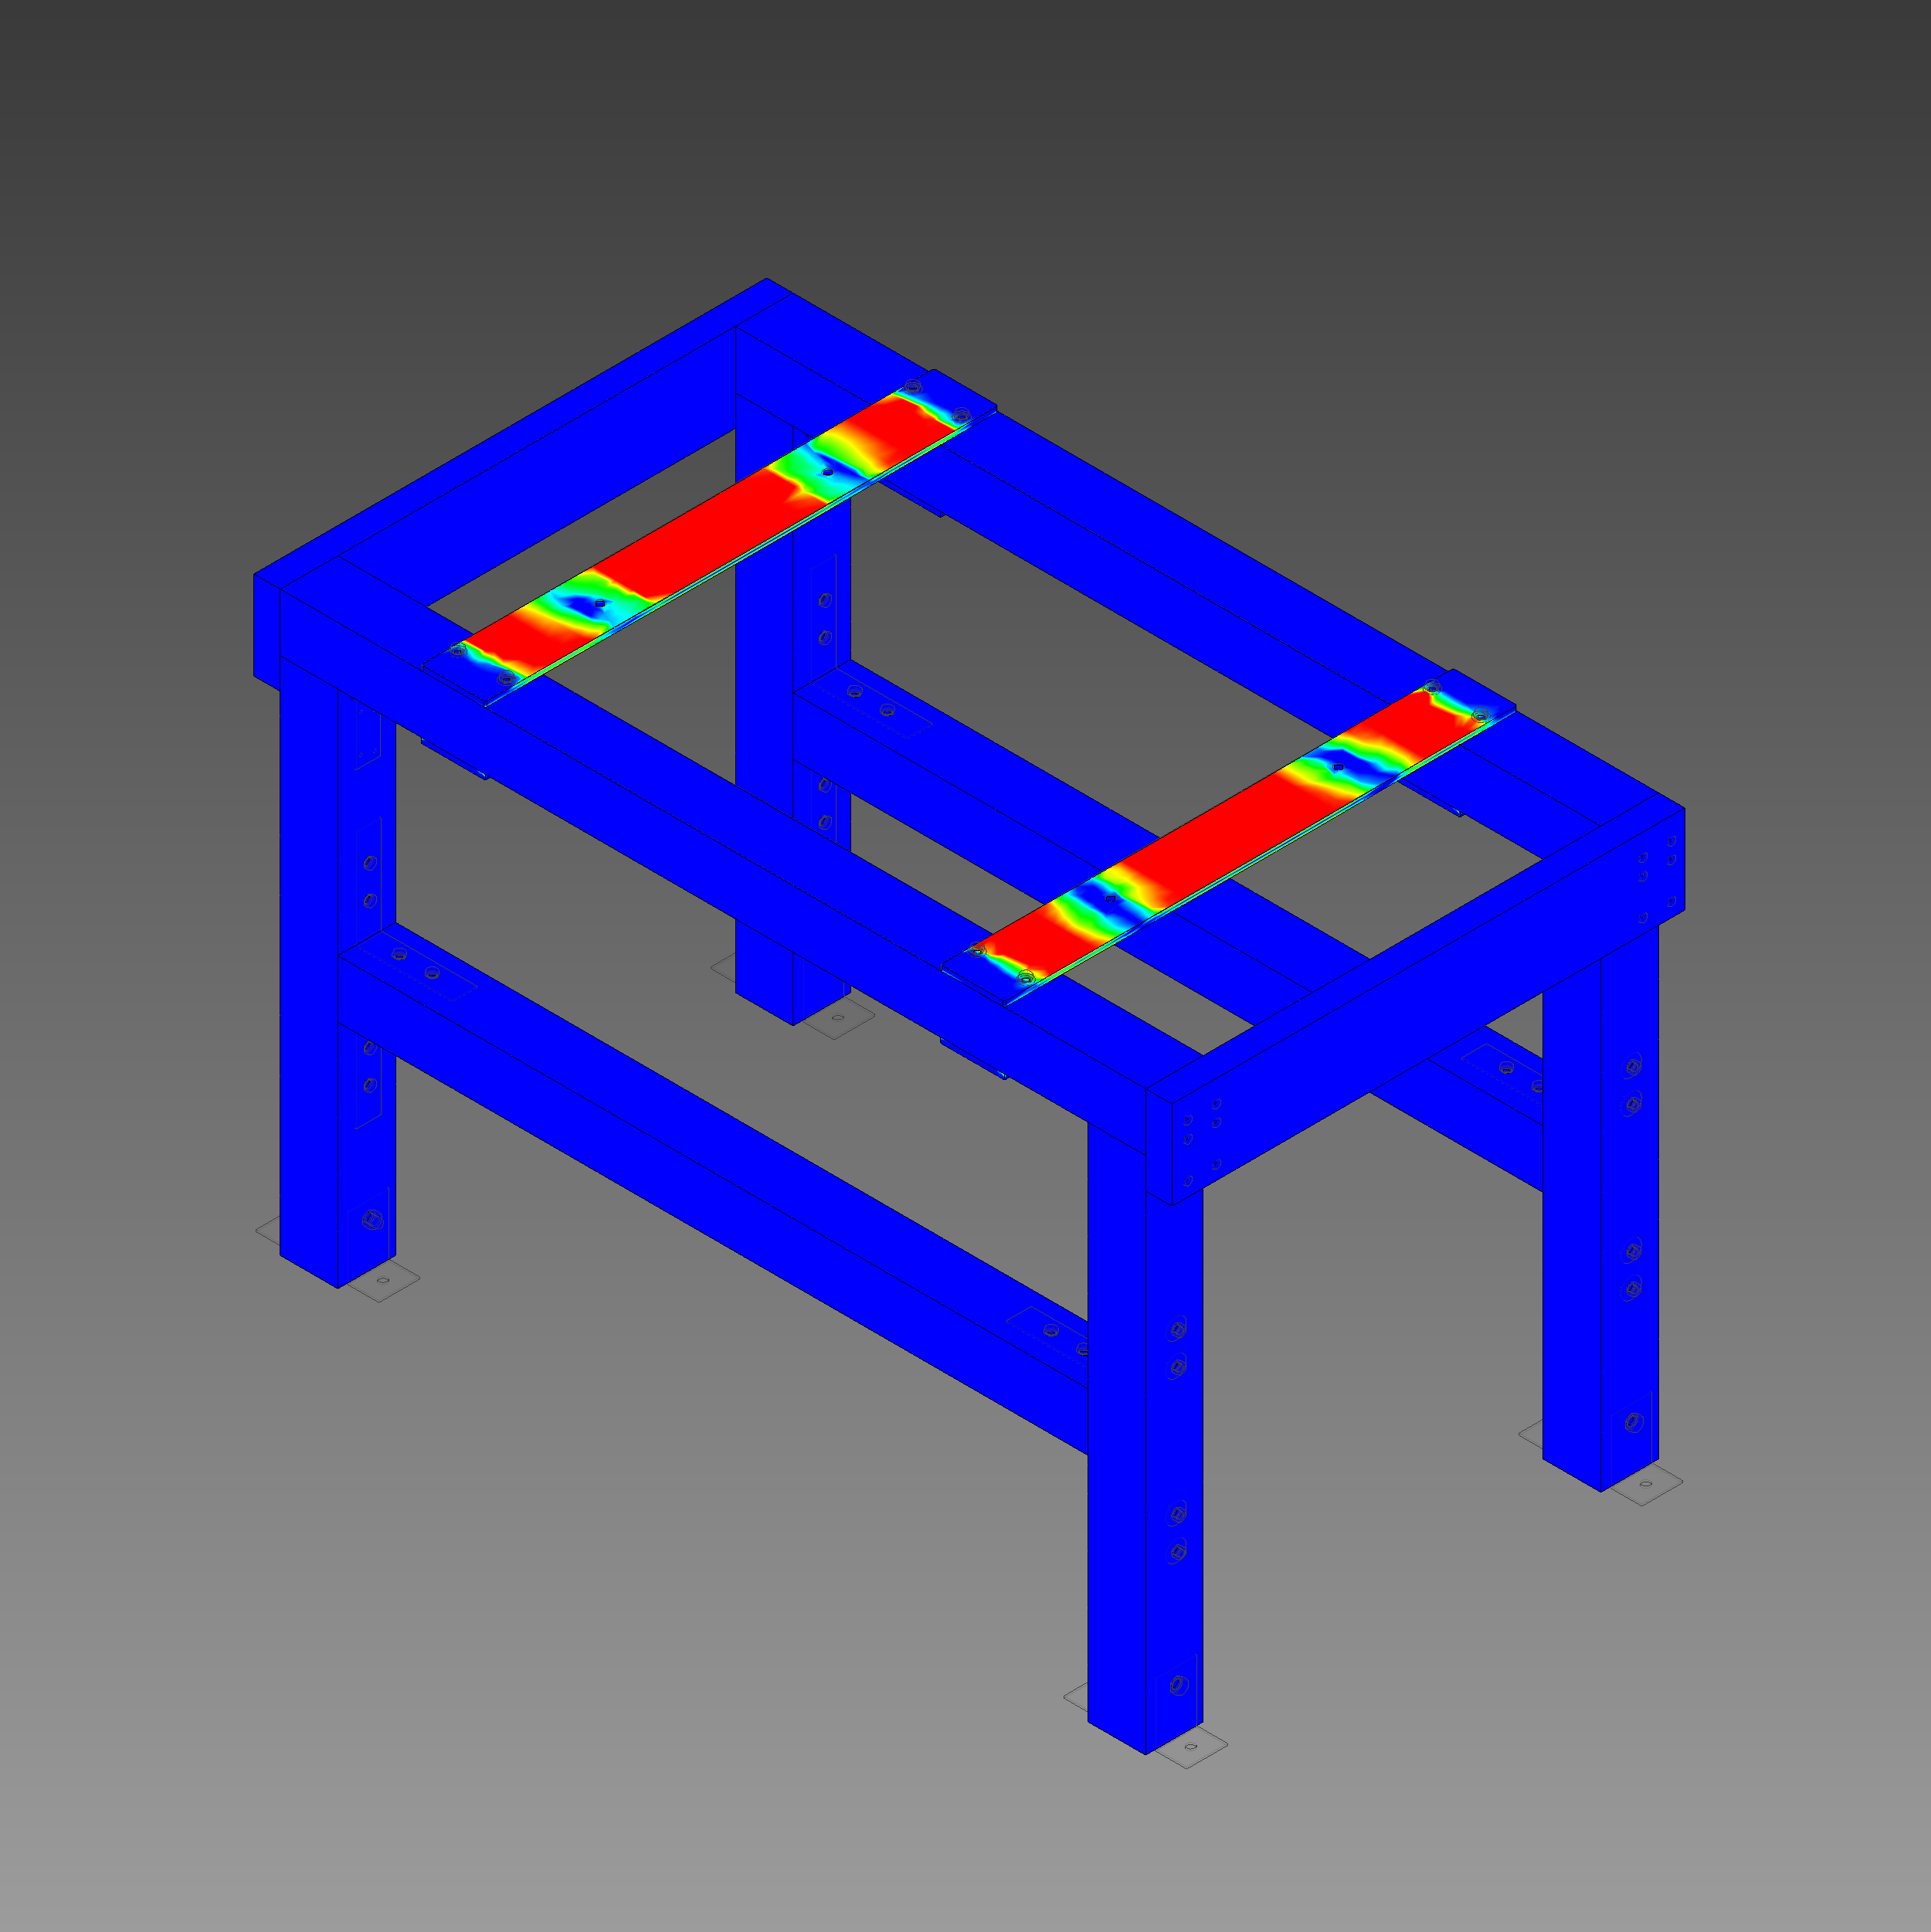
\includegraphics[width=1\linewidth]{Imagenes/rmesa_gen.png}
		\caption{}\label{fig:rmesa_gen}
	\end{subfigure}%
	\begin{subfigure}{0.49\linewidth}
		\centering
		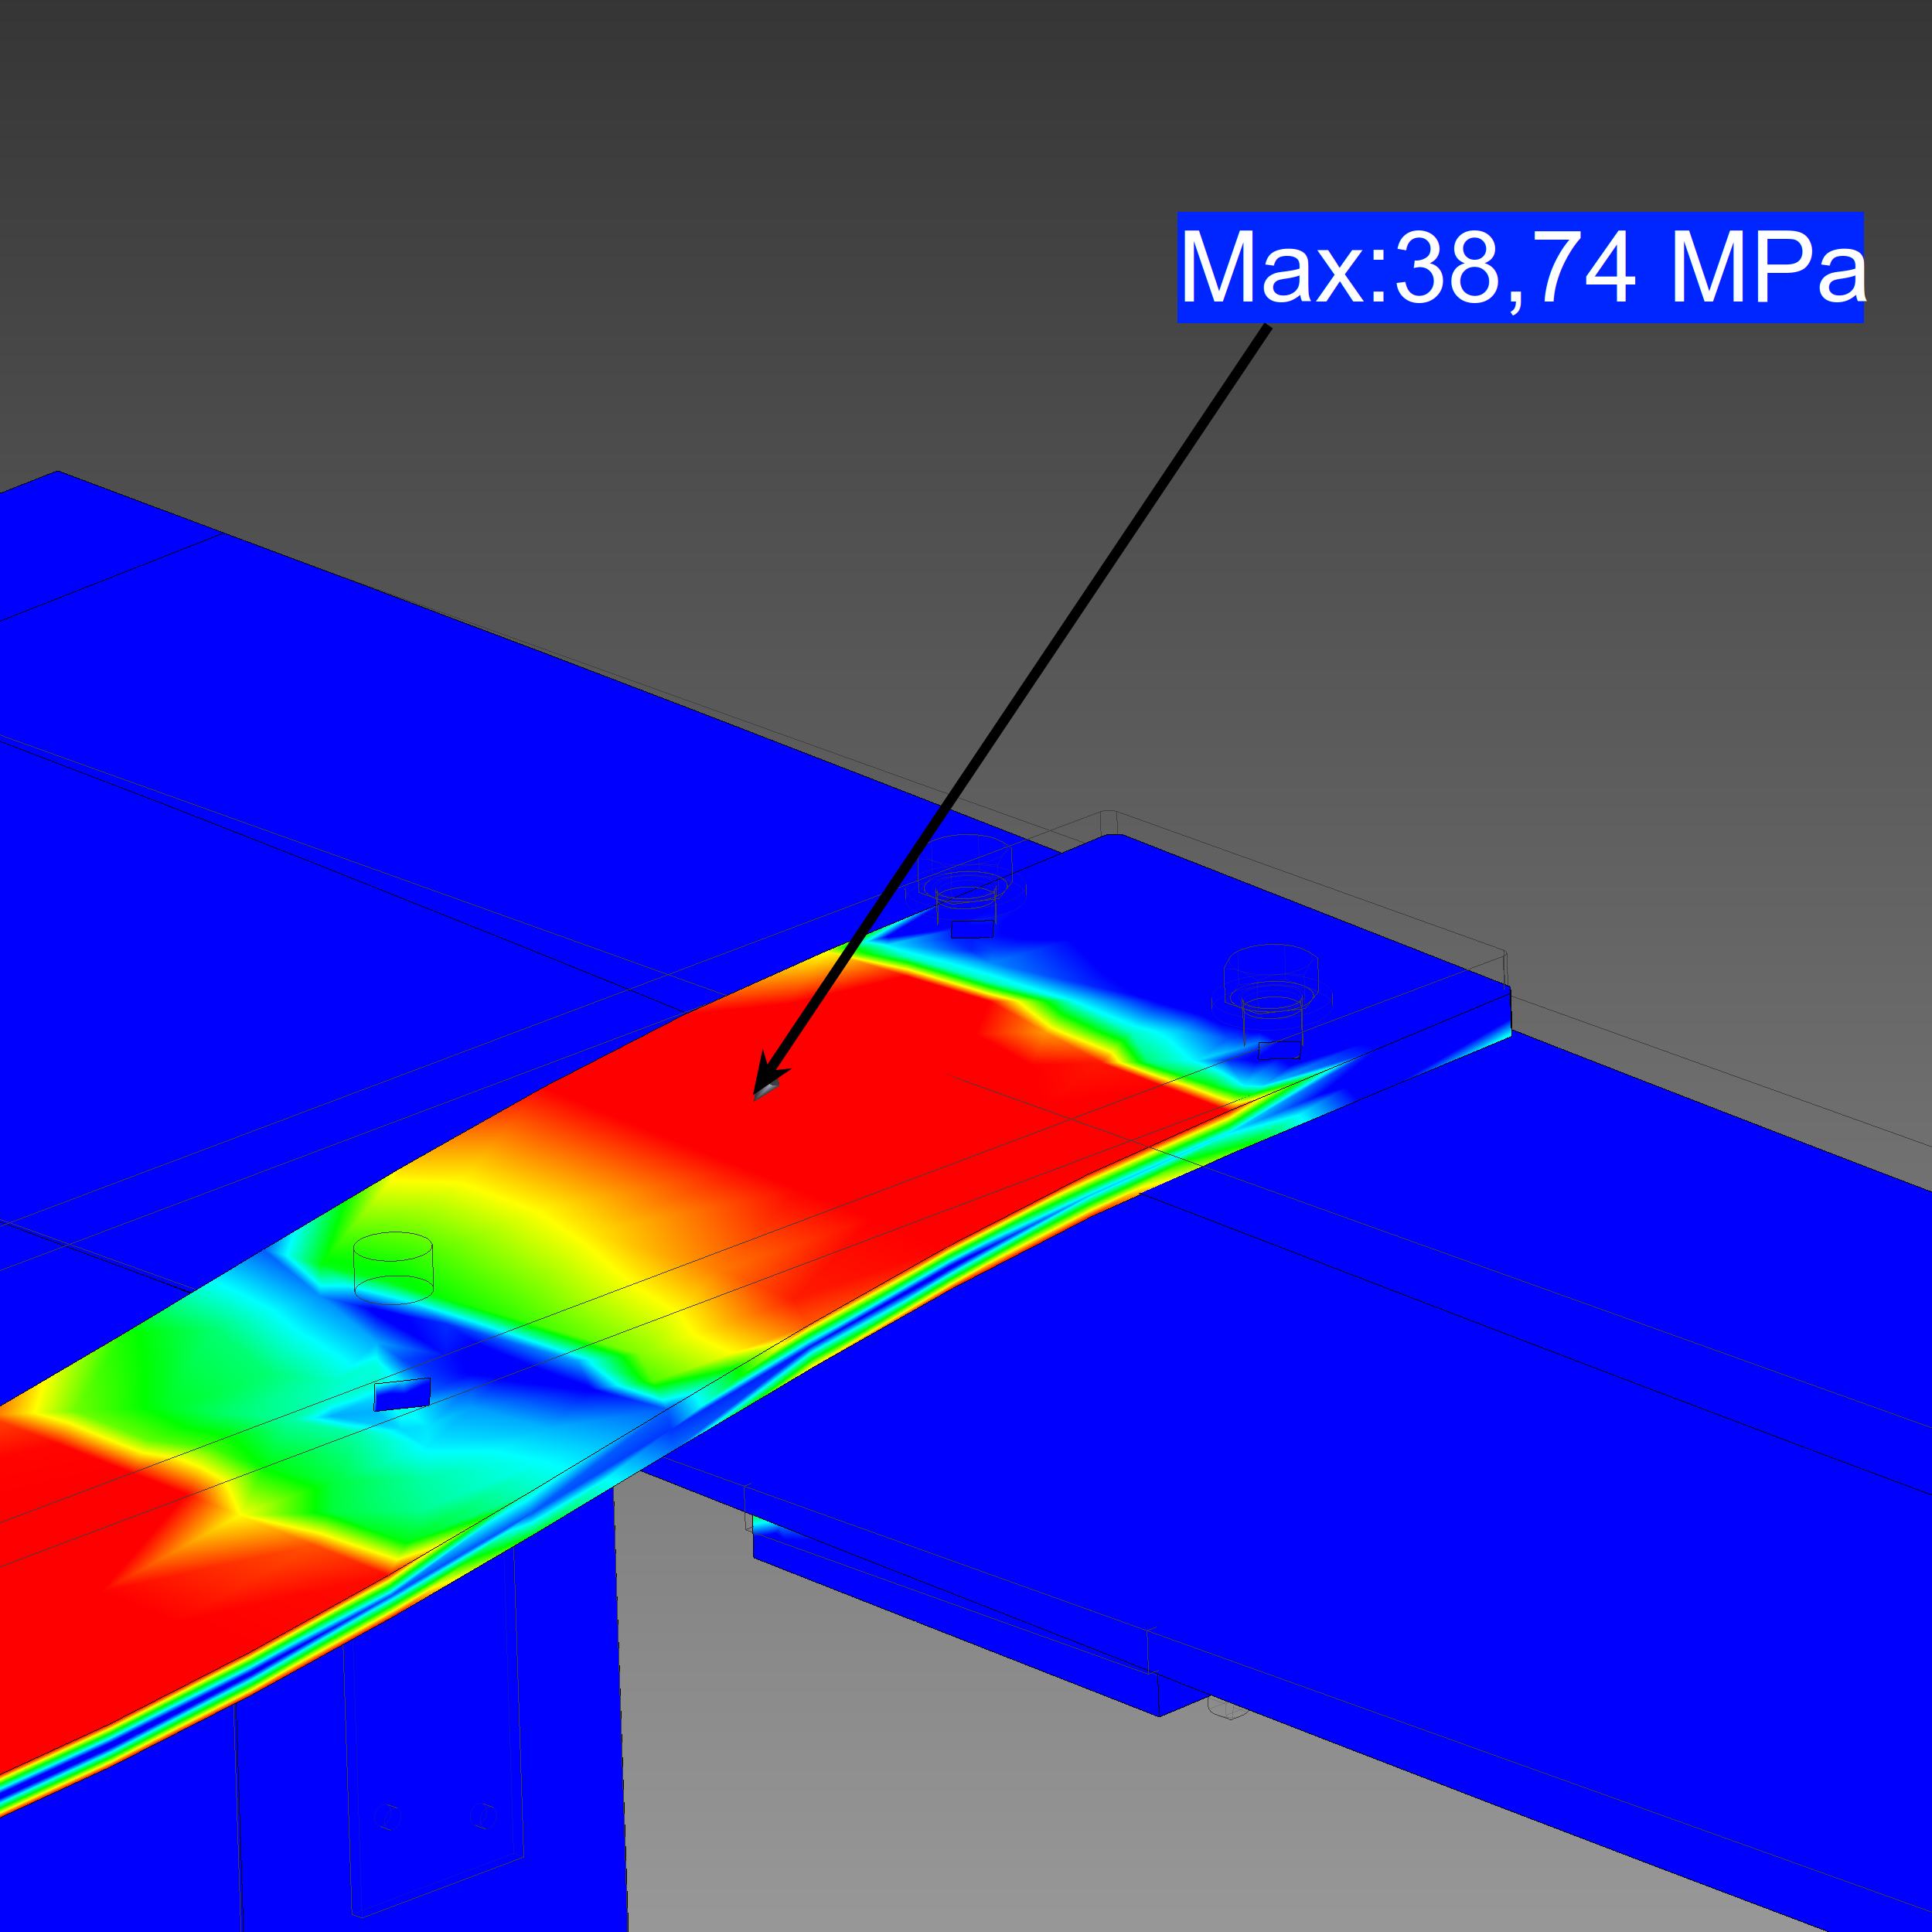
\includegraphics[width=1\linewidth]{Imagenes/rmesa_det.png}
		\caption{}\label{fig:rmesa_det}
	\end{subfigure}
\caption{La figura (a) muestra los esfuerzos de von Mises provocados por la mesa de fatiga sobre la estructura. La figura (b) es un detalle del esfuerzo de von Mises máximo, que se produce en los extremos de la pletina de acero.}
\label{fig:resultados_mesa}
\end{figure}
El esfuerzo de von Mises máximo obtenido es de 38,74 MPa, ubicados donde muestra la fig. \ref{fig:rmesa_det}, dando como resultado un factor de seguridad igual a 3,38 (-). La deformación máxima se encuentra en la mitad de la pletina de acero, siendo 1,038 mm.

En definitiva, tanto los resultados obtenidos por la simulación como los obtenidos a través en base al cálculo y la norma de madera, nos indican que la madera no tendrá problemas en soportar la carga estática de la máquina por su sobredimensionamiento. Se confirman los puntos críticos del diseño general y, por último, los resultados del análisis modal revelan que no habrán problemas con la frecuencia natural de la estructura y el funcionamiento de la máquina de fatiga.

\section{Modelo del sistema}

\subsection{Comportamiento del modelo}
Con la caracterización y el levantamiento de información de los distintos componentes, junto a la elección de $c_1$, $c_2$ y de las variables de la función $\phi$, nos permite resolver y obtener valores del movimiento lineal, angular y la carga a la que está sometida la probeta. El tiempo de integración para cada una de las soluciones será entre 0 y 8 segundos. Se utilizará una tolerancia relativa y absoluta de $10^{-8}$. En consecuencia, al resolver el sistema de ecuaciones \ref{eq:mov_matriz} a través de los códigos de la sección \ref{sec:sol_part}, se obtiene la posición ($y,\theta$) y la velocidad ($\dot{y},\dot{\theta}$) del brazo de carga respecto a su centro de masa. Las figuras \ref{fig:yt_2} y \ref{fig:ytp_2} muestran las curvas de cada coordenada.

Utilizando la ec. \ref{eq:fuerza_probeta} para cada valor de $y_2(t)$, se obtiene la carga aplicada sobre la probeta $F(t)$ a lo largo del tiempo. La fig. \ref{fig:f_2} muestra la curva de esta fuerza a través del tiempo para la configuración n$^{\circ}$ 38 ($\Delta m = 14.5020$ g).

En el conjunto de figuras \ref{fig:yt_2} y \ref{fig:ytp_2} se aprecia como el sistema tiene dos etapas principales: (a) la estabilización y reposo del sistema y (b) el inicio de la función $\phi$. (a) La primera etapa comienza en $t=0$, cuando se encuentra en un estado inicial $(y, \dot{y}, \theta, \dot{\theta}) = (0,0,0,0)$. Tanto la probeta y las barras en voladizo se encuentran sólo bajo la acción de la gravedad, por lo tanto caen y comienzan a oscilar en torno a su posición de reposo, sin embargo, este movimiento decae a medida que avanza el tiempo producto de los amortiguadores. La velocidad de decaimiento de la vibración inicial está determinado por el valor de $c_1$ y $c_2$, teniendo un comportamiento subamortiguado. (b) A continuación, desde el segundo 2 la función $\phi$ comienza a acelerar suavemente hasta llegar a la velocidad $\omega_{max} = 1500$ rpm, punto en el cual la vibración es constante y estable en el tiempo. A partir de este punto, se extraen la información respectiva de la fuerza máxima, media y alternante, utilizando las ecuaciones \ref{eq:f_max}, \ref{eq:f_m} y \ref{eq:f_a}. 

\begin{figure}[h]
\centering
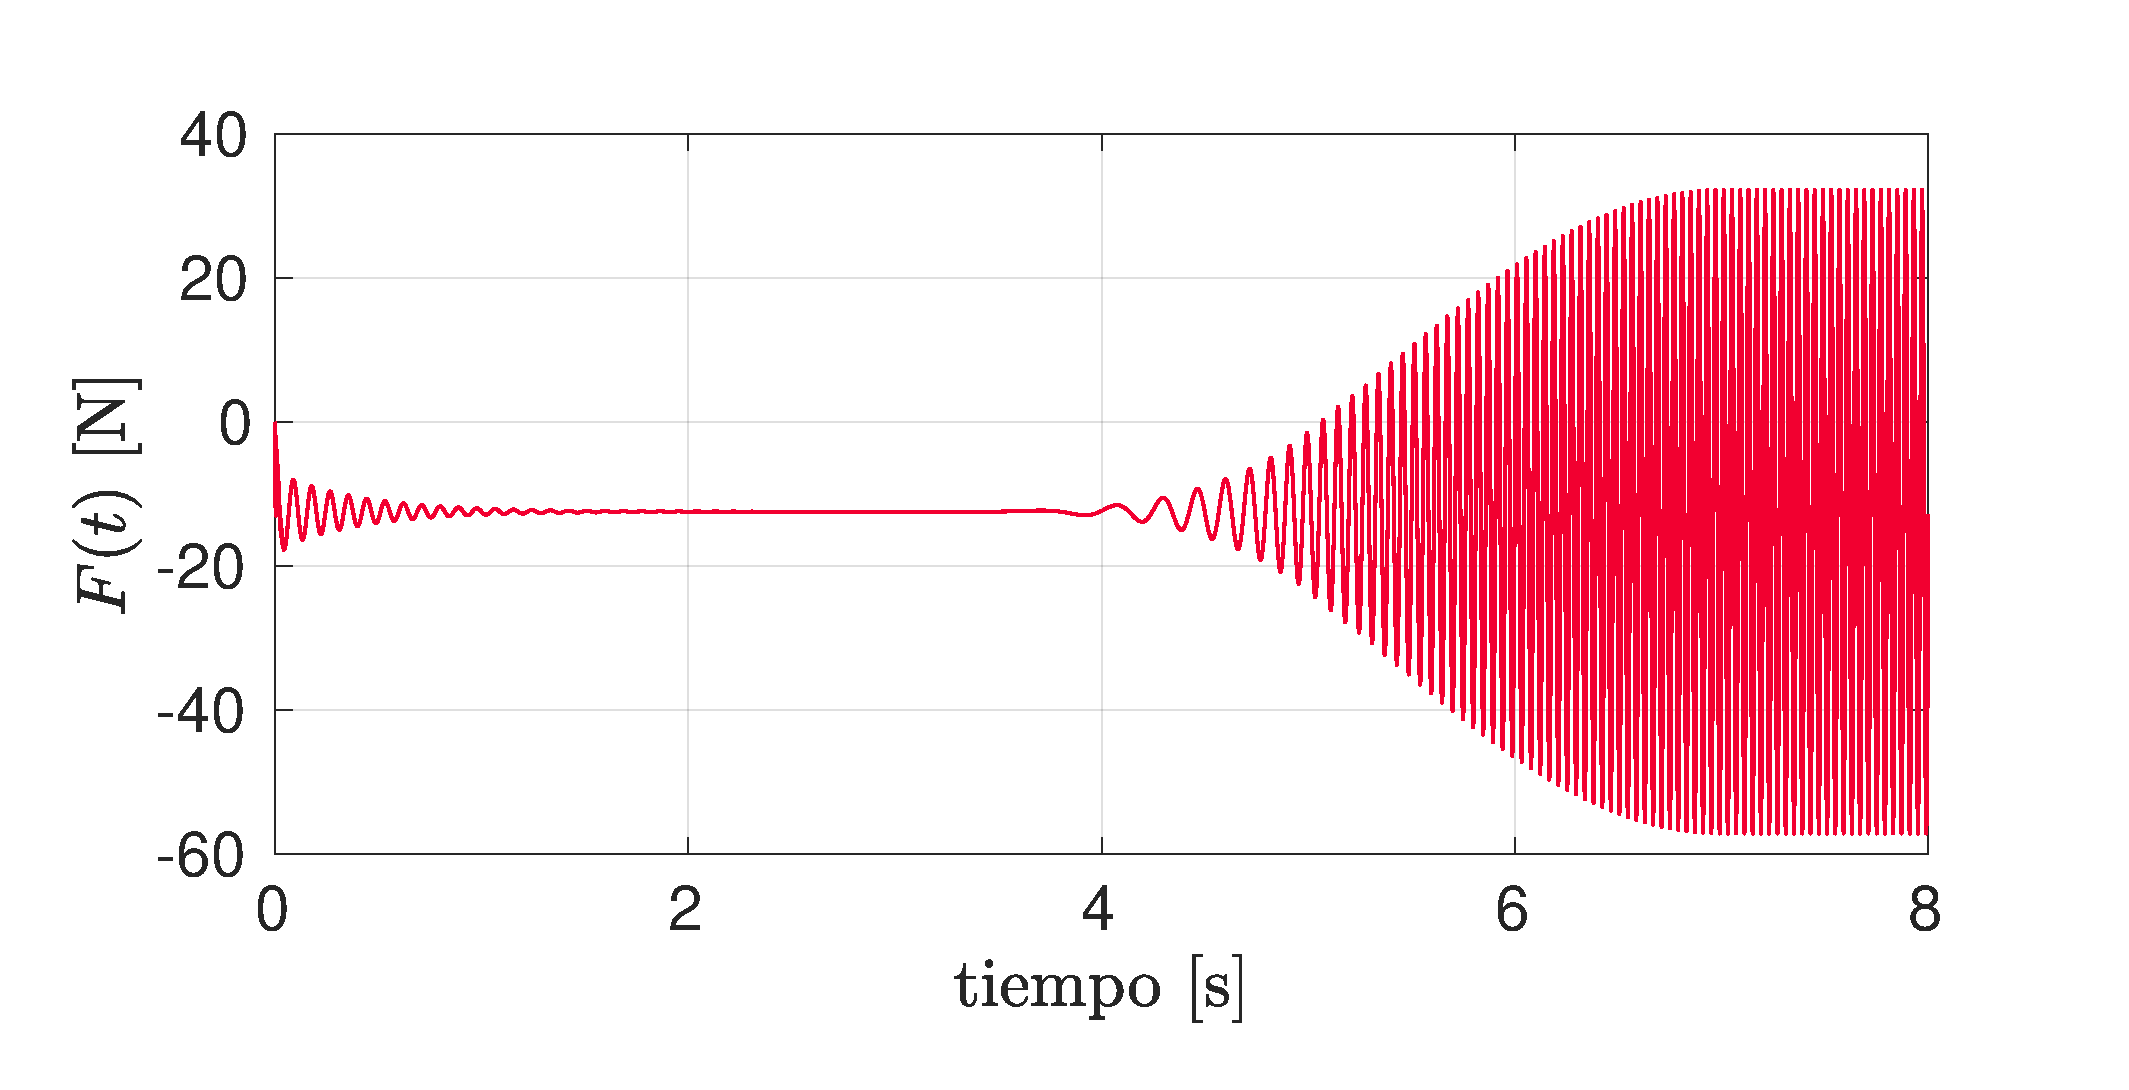
\includegraphics[width=0.95\linewidth, trim={0cm 1cm 2cm 1cm},clip]{Imagenes/f_2.pdf}
\caption{Fuerza aplicada sobre la probeta $F(t)$ en el tiempo para la combinación n$^{\circ}$ 38, $\Delta m = 14.5020$ g.}
\label{fig:f_2}
\end{figure}

\begin{figure}[p]
\centering
	\begin{subfigure}{1\linewidth}
		\centering
		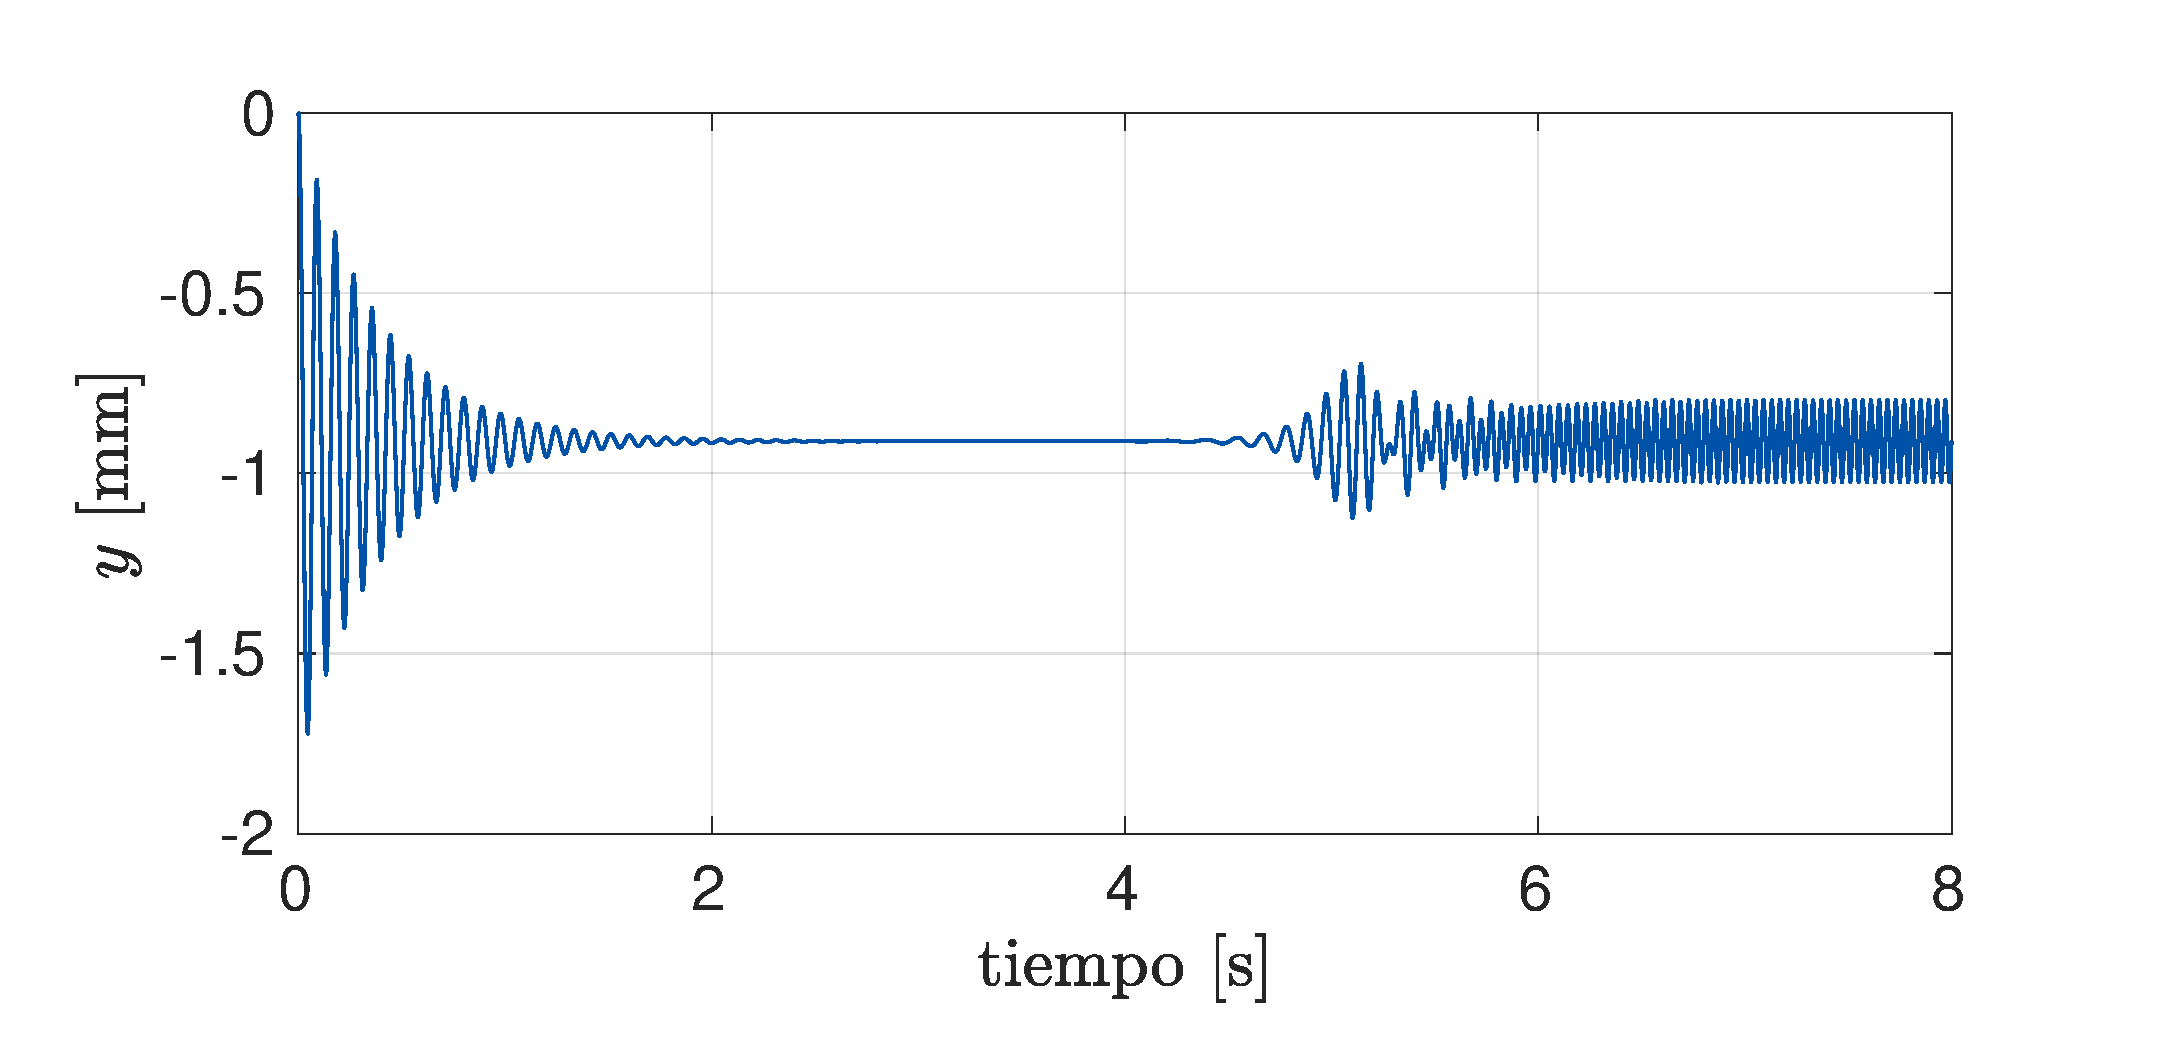
\includegraphics[width=1\linewidth]{Imagenes/y_2.pdf}
		\caption{}\label{fig:y_2}
	\end{subfigure}
	\begin{subfigure}{1\linewidth}
		\centering
		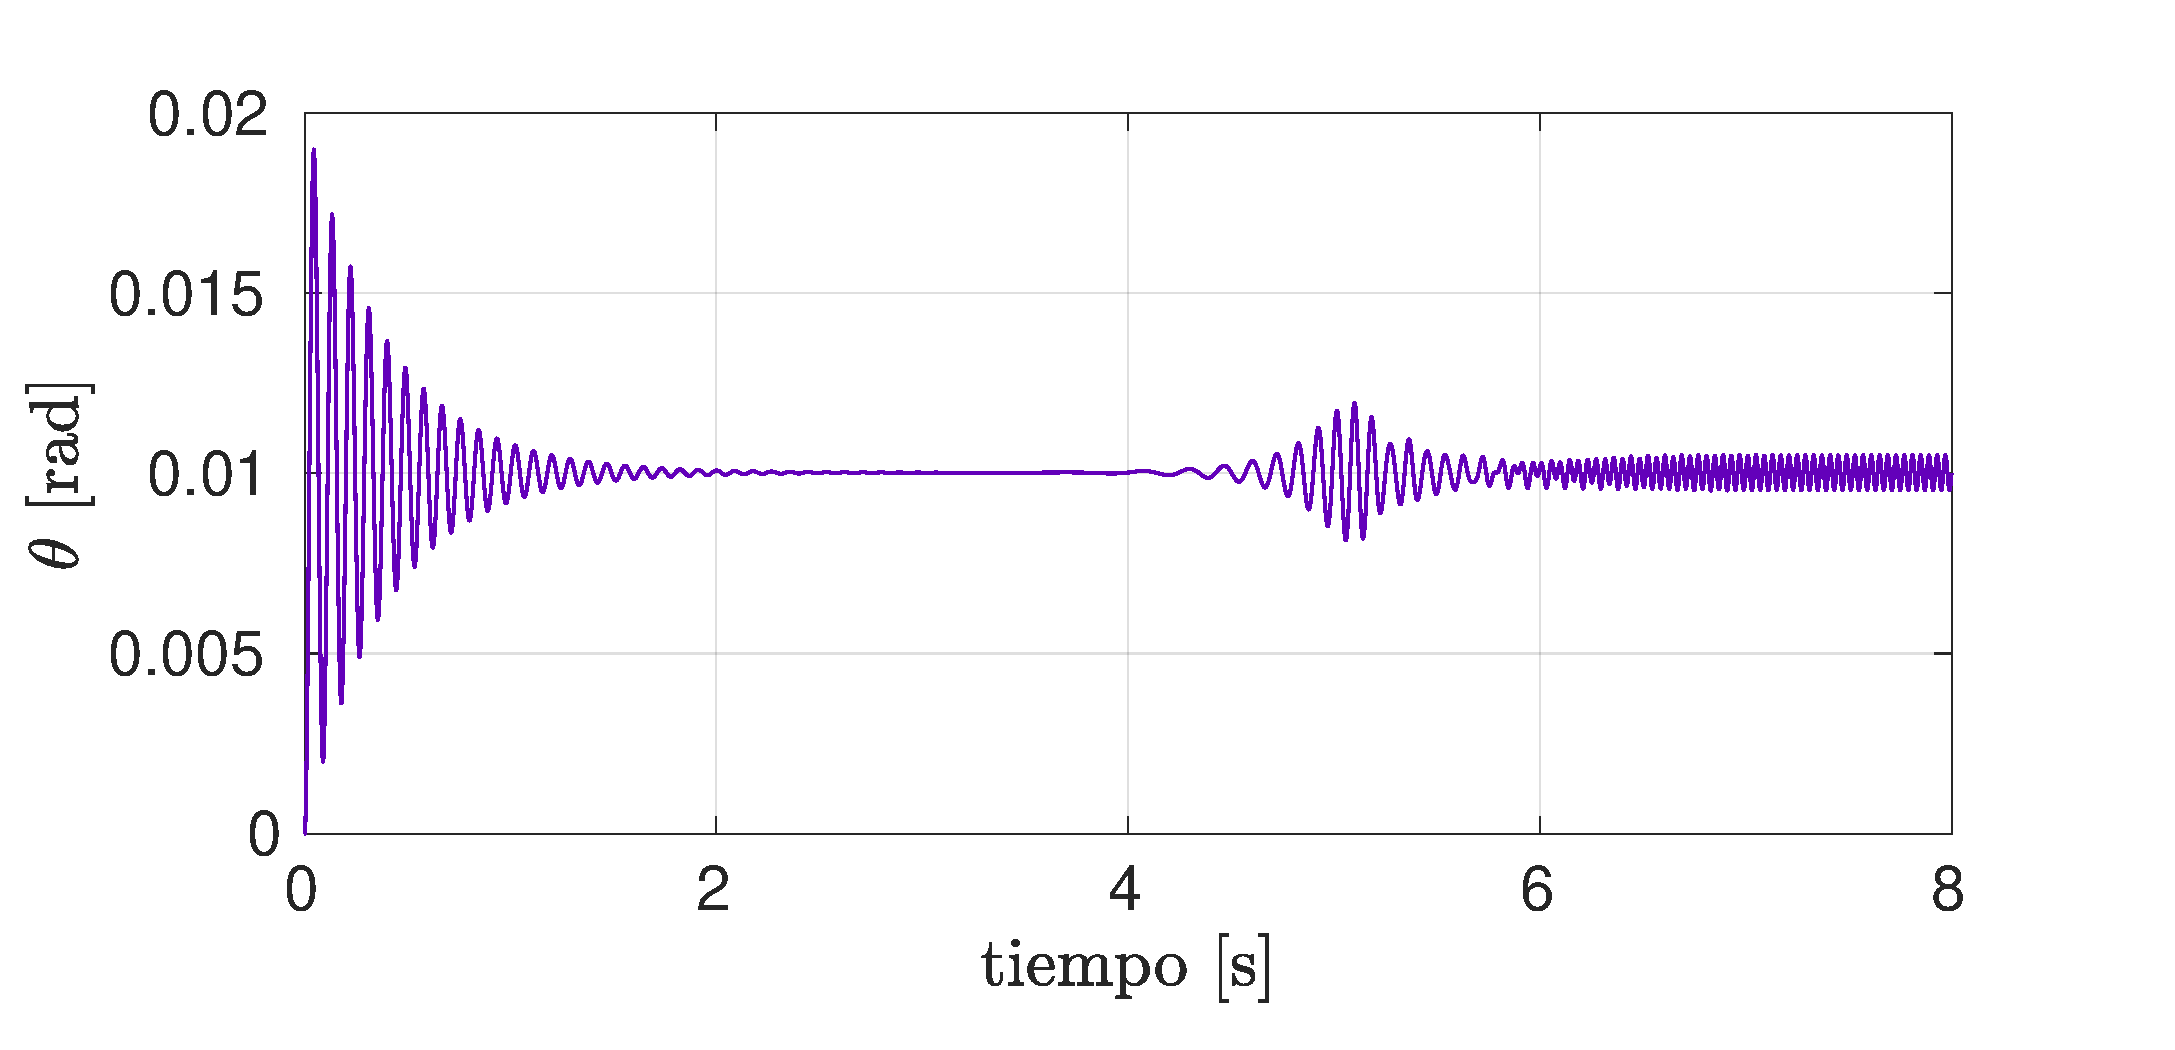
\includegraphics[width=1\linewidth]{Imagenes/t_2.pdf}
		\caption{}\label{fig:t_2}
	\end{subfigure}
\par\bigskip
\caption{Desplazamiento en el tiempo respecto (a) al eje $y$ y (b) al eje $\theta$ del centro de masa del brazo de carga. Gráficas para un desbalanceo $\Delta m = 92.3469$ g }
\label{fig:yt_2}
\end{figure}


\begin{figure}[p]
\centering
	\begin{subfigure}{1\linewidth}
		\centering
		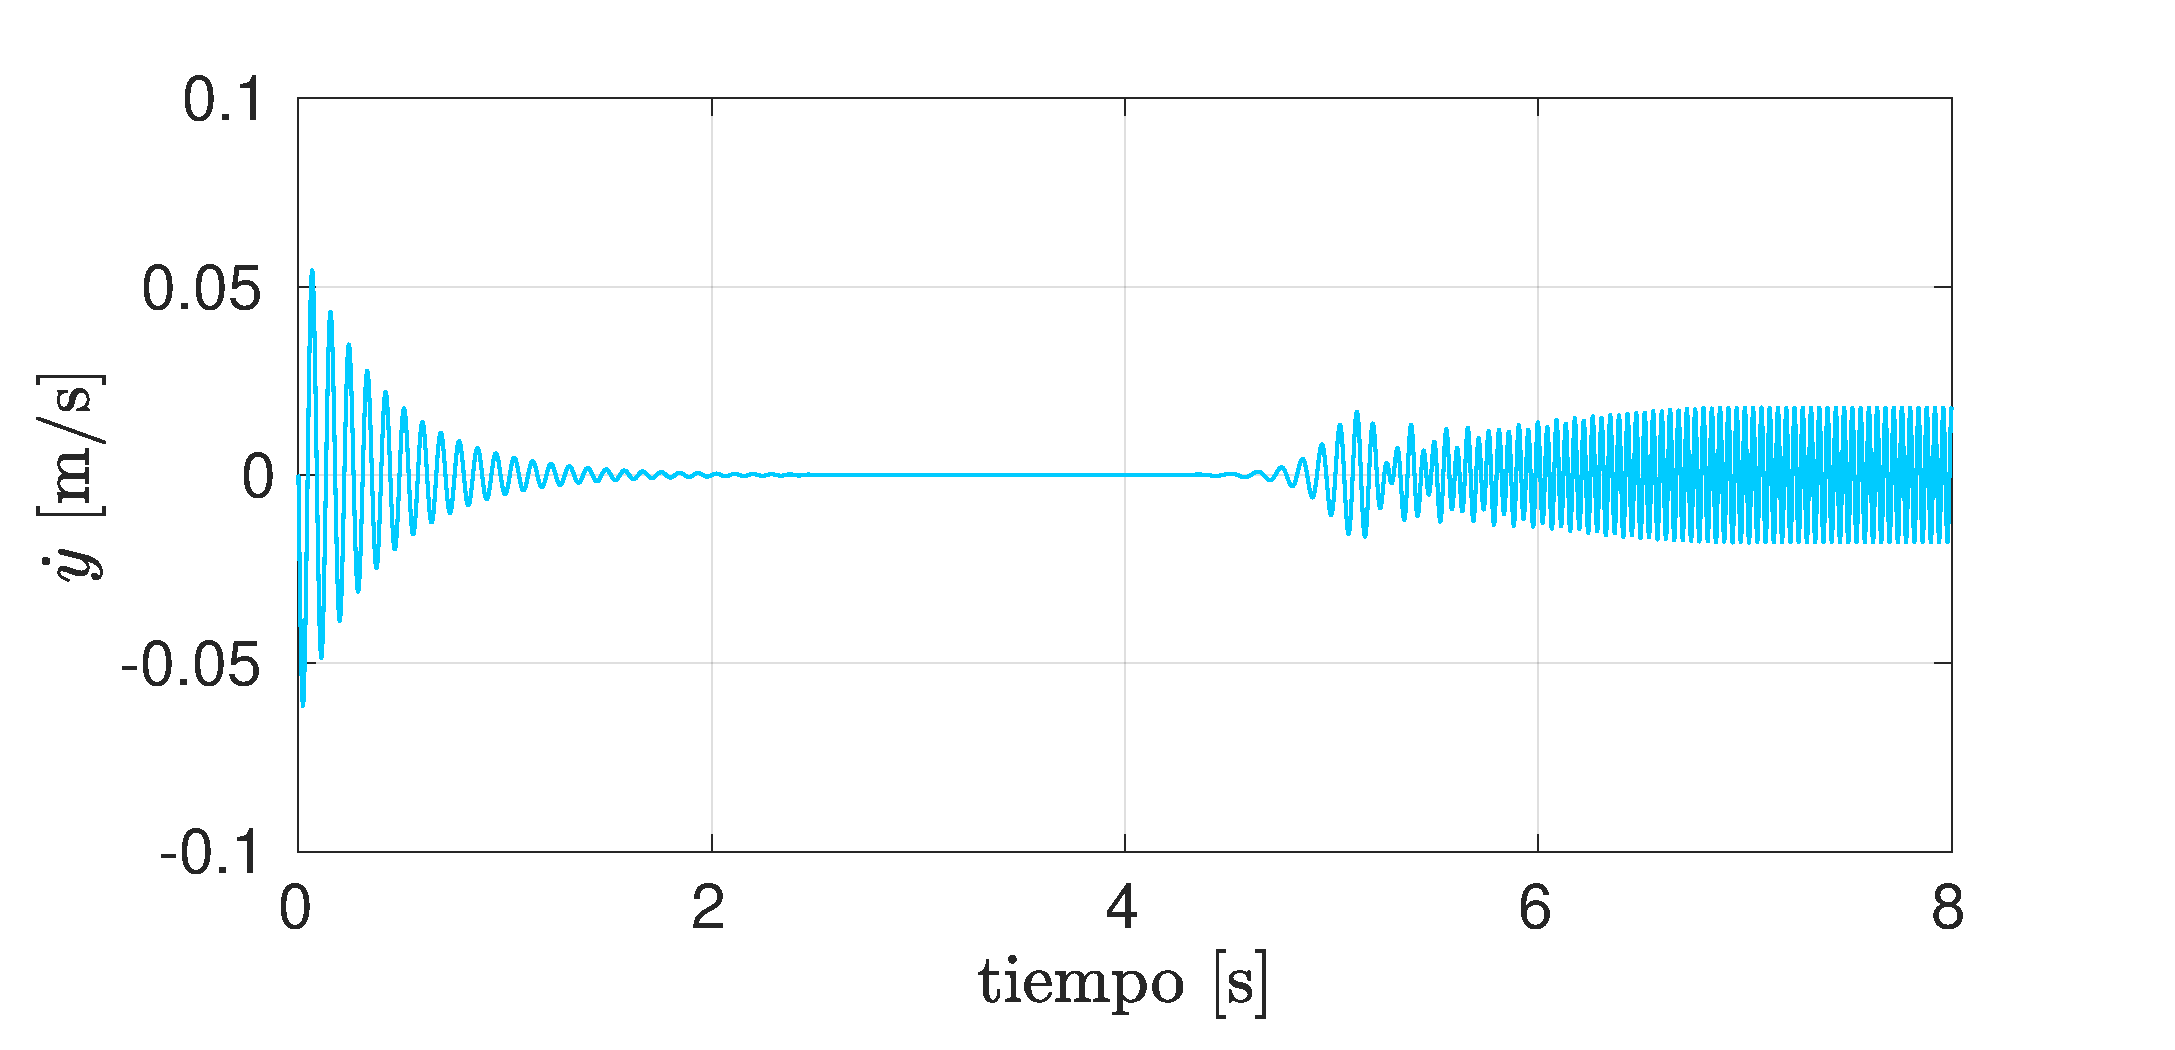
\includegraphics[width=1\linewidth]{Imagenes/yp_2.pdf}
		\caption{}\label{fig:yp_2}
	\end{subfigure}
	\begin{subfigure}{1\linewidth}
		\centering
		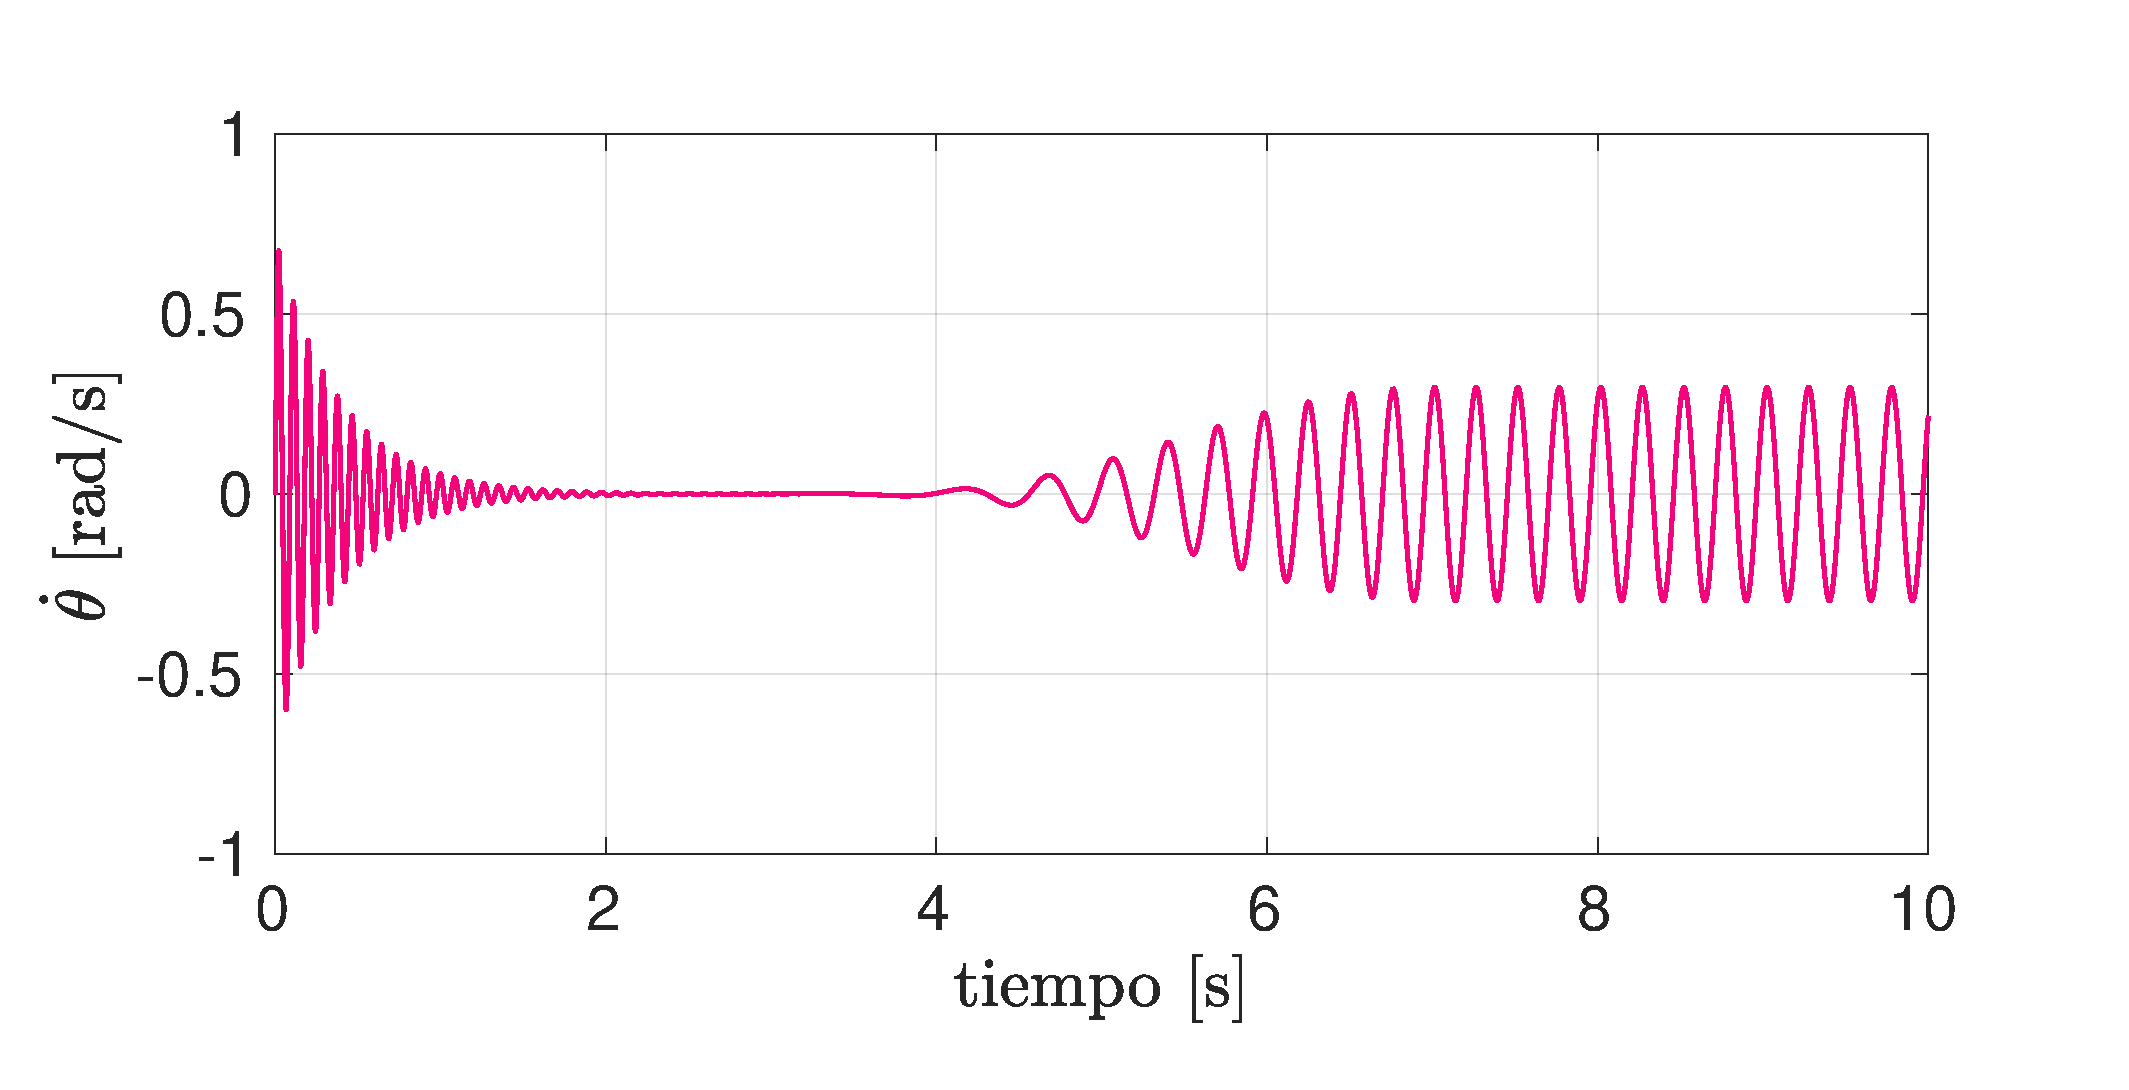
\includegraphics[width=1\linewidth]{Imagenes/tp_2.pdf}
		\caption{}\label{fig:tp_2}
	\end{subfigure}
\par\bigskip
\caption{Velocidad respecto la tiempo (a) en el eje $y$ y (b) el eje $\theta$ del centro de masa del brazo de carga. Gráficas para un desbalanceo $\Delta m = 92.3469$ g}
\label{fig:ytp_2}
\end{figure}

%\begin{figure}[h]
%\centering
%	\begin{subfigure}{1\linewidth}
%		\centering
%		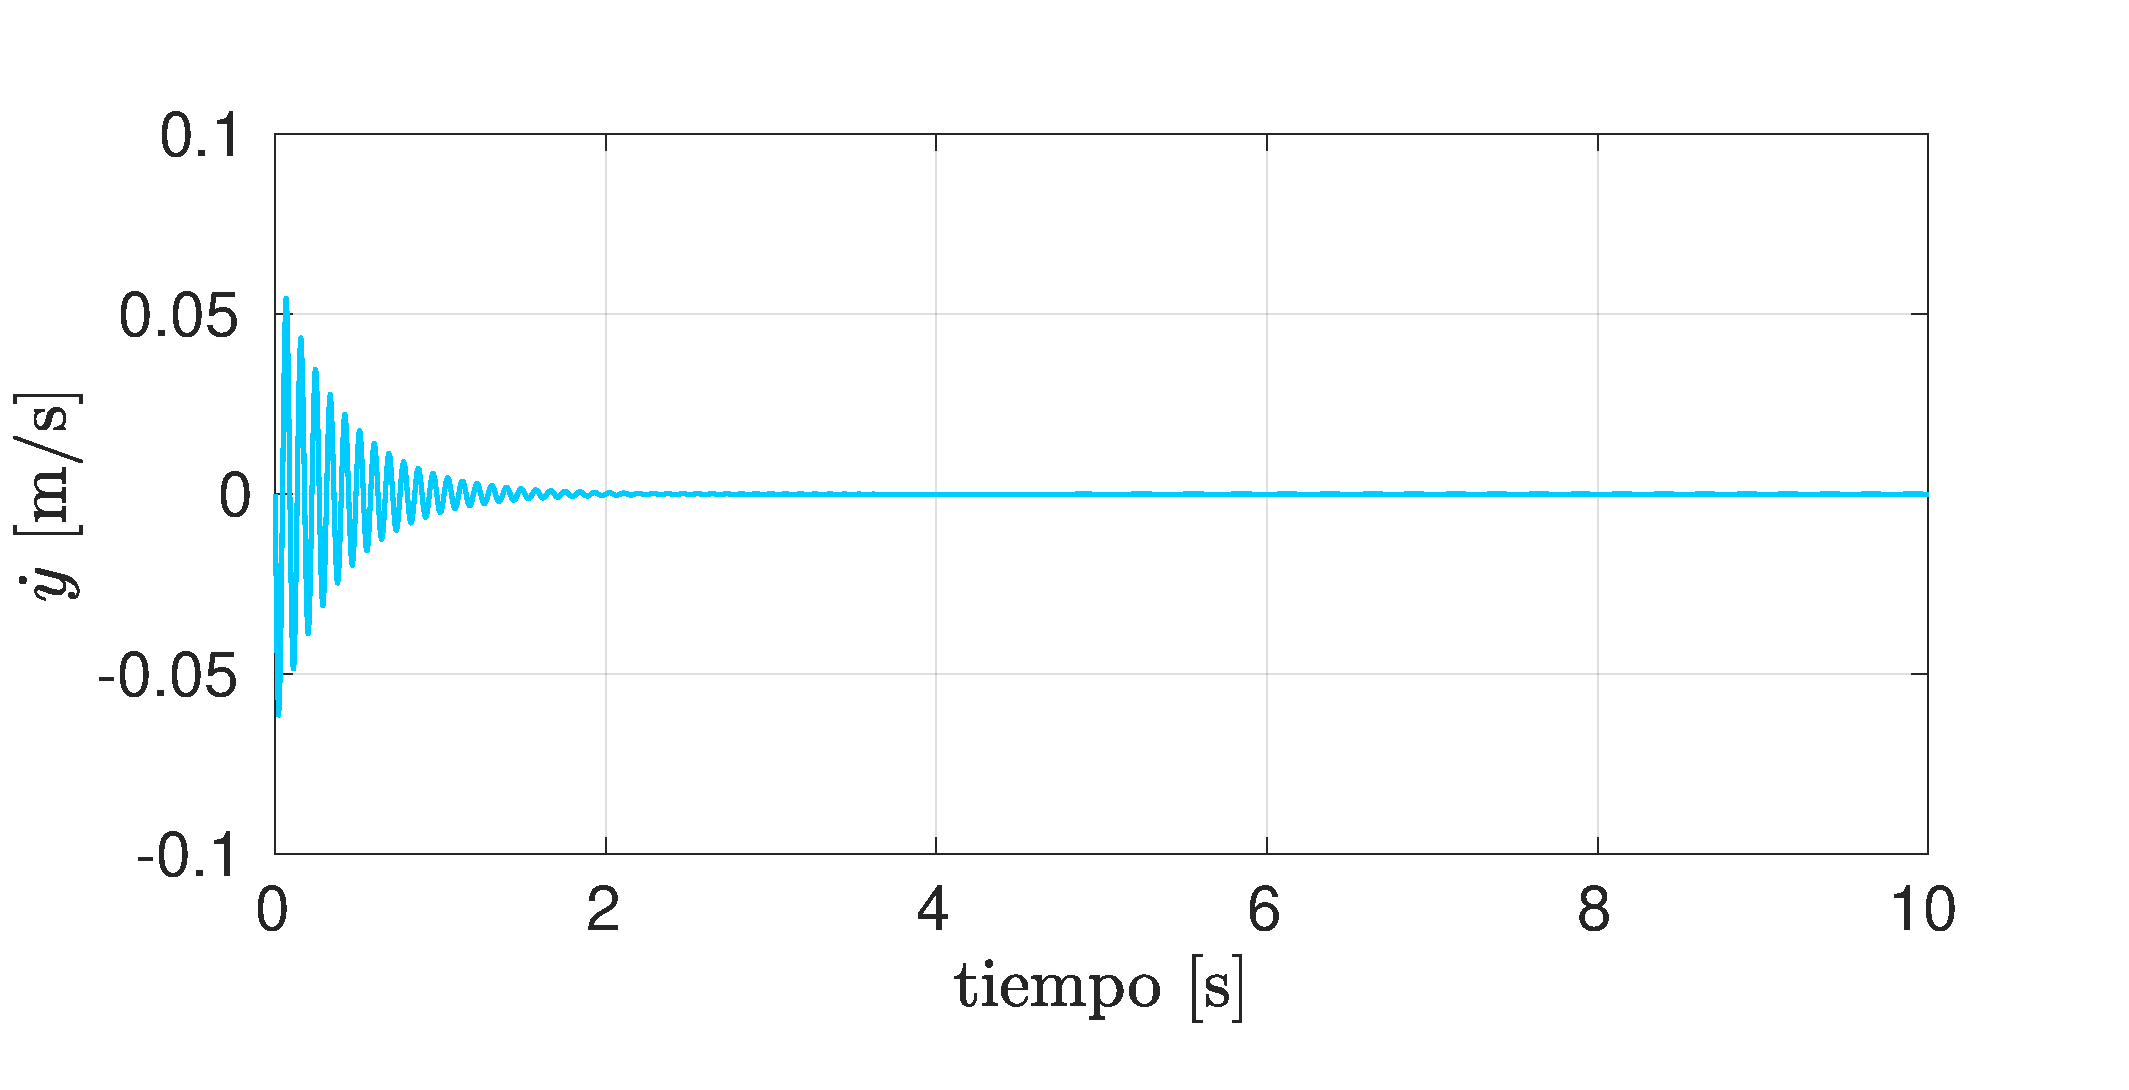
\includegraphics[width=1\linewidth]{Imagenes/yp_1.pdf}
%		\caption{}\label{fig:yp_1}
%	\end{subfigure}
%	\begin{subfigure}{1\linewidth}
%		\centering
%		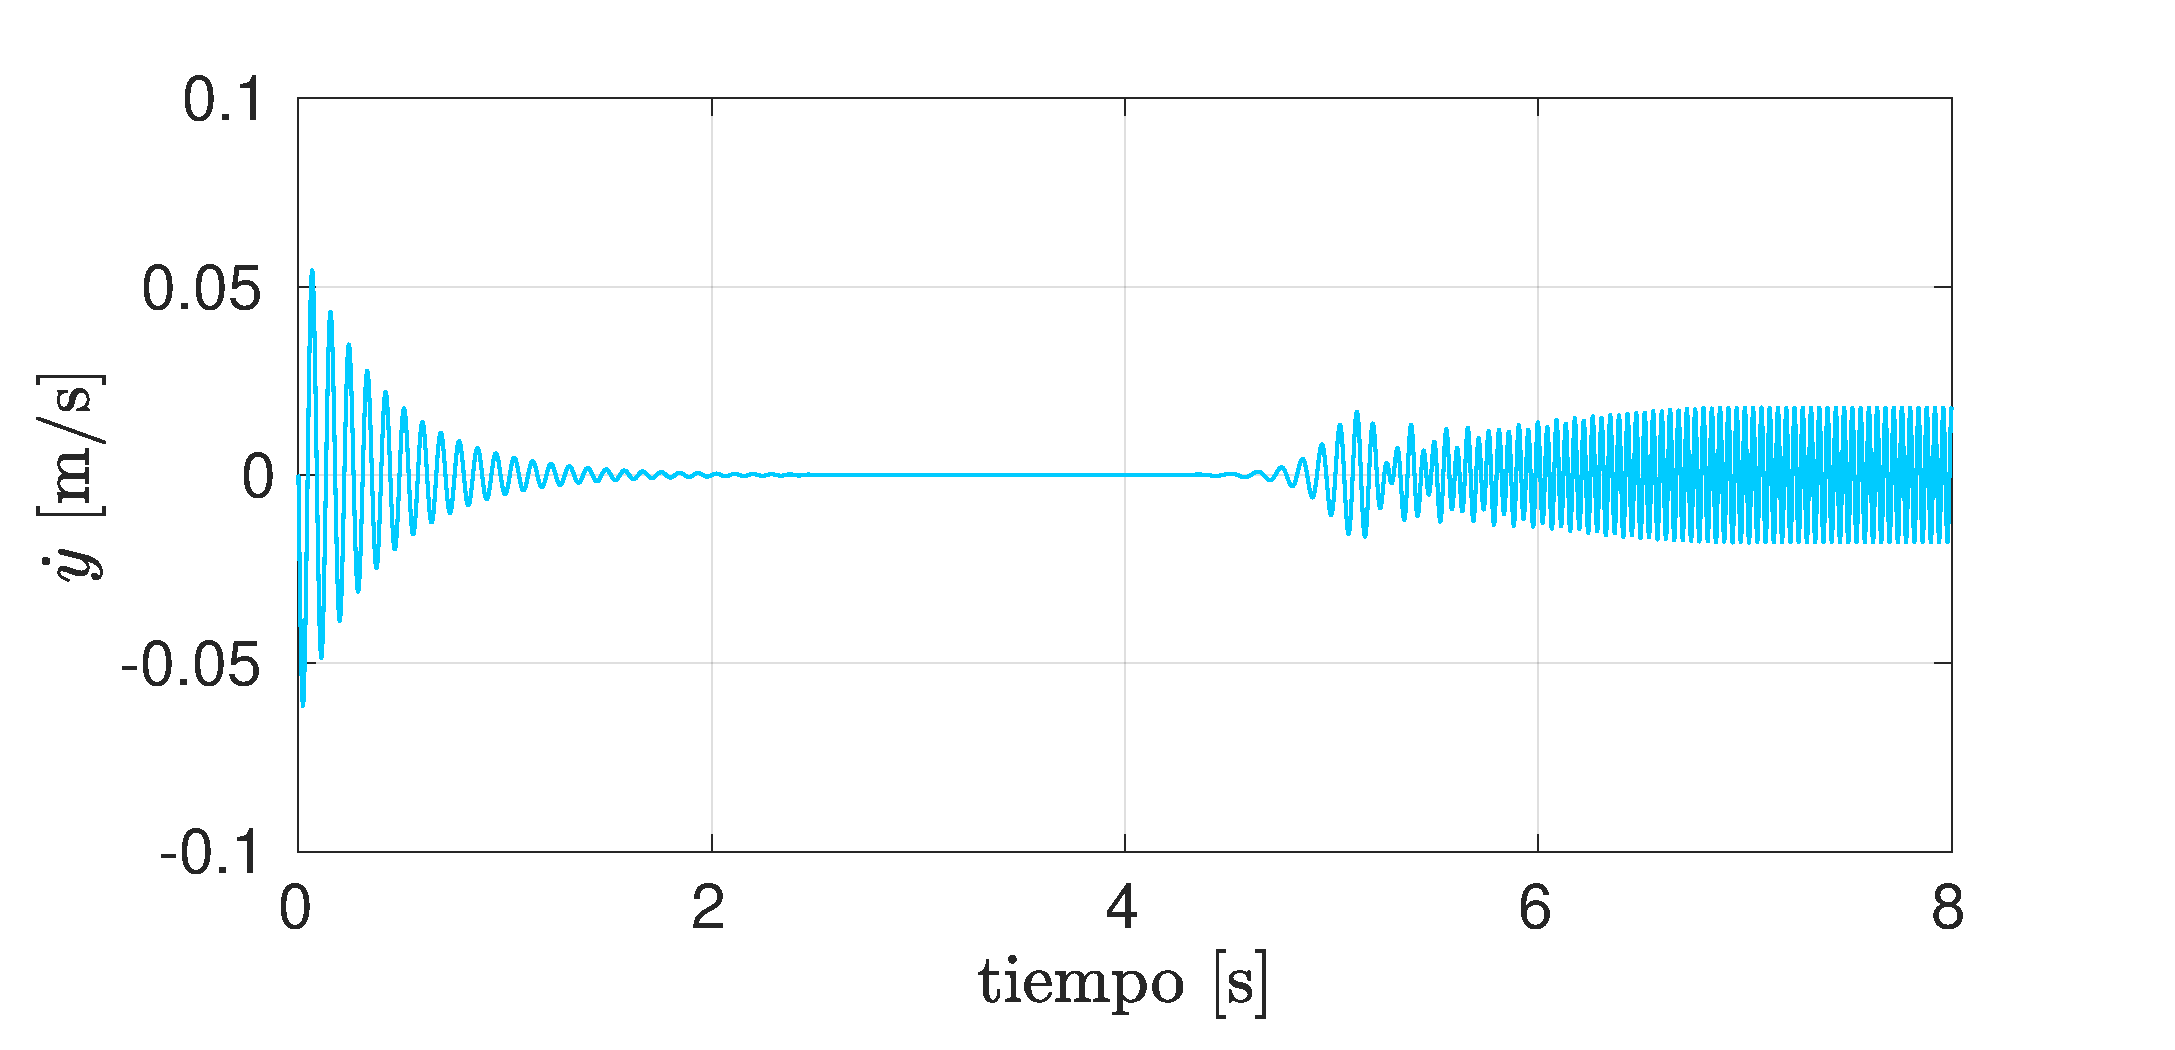
\includegraphics[width=1\linewidth]{Imagenes/yp_2.pdf}
%		\caption{}\label{fig:yp_2}
%	\end{subfigure}
%\par\bigskip
%\caption{sadfafssafdasf}
%\label{fig:vely_12}
%\end{figure}
%
%\begin{figure}[h]
%\centering
%	\begin{subfigure}{1\linewidth}
%		\centering
%		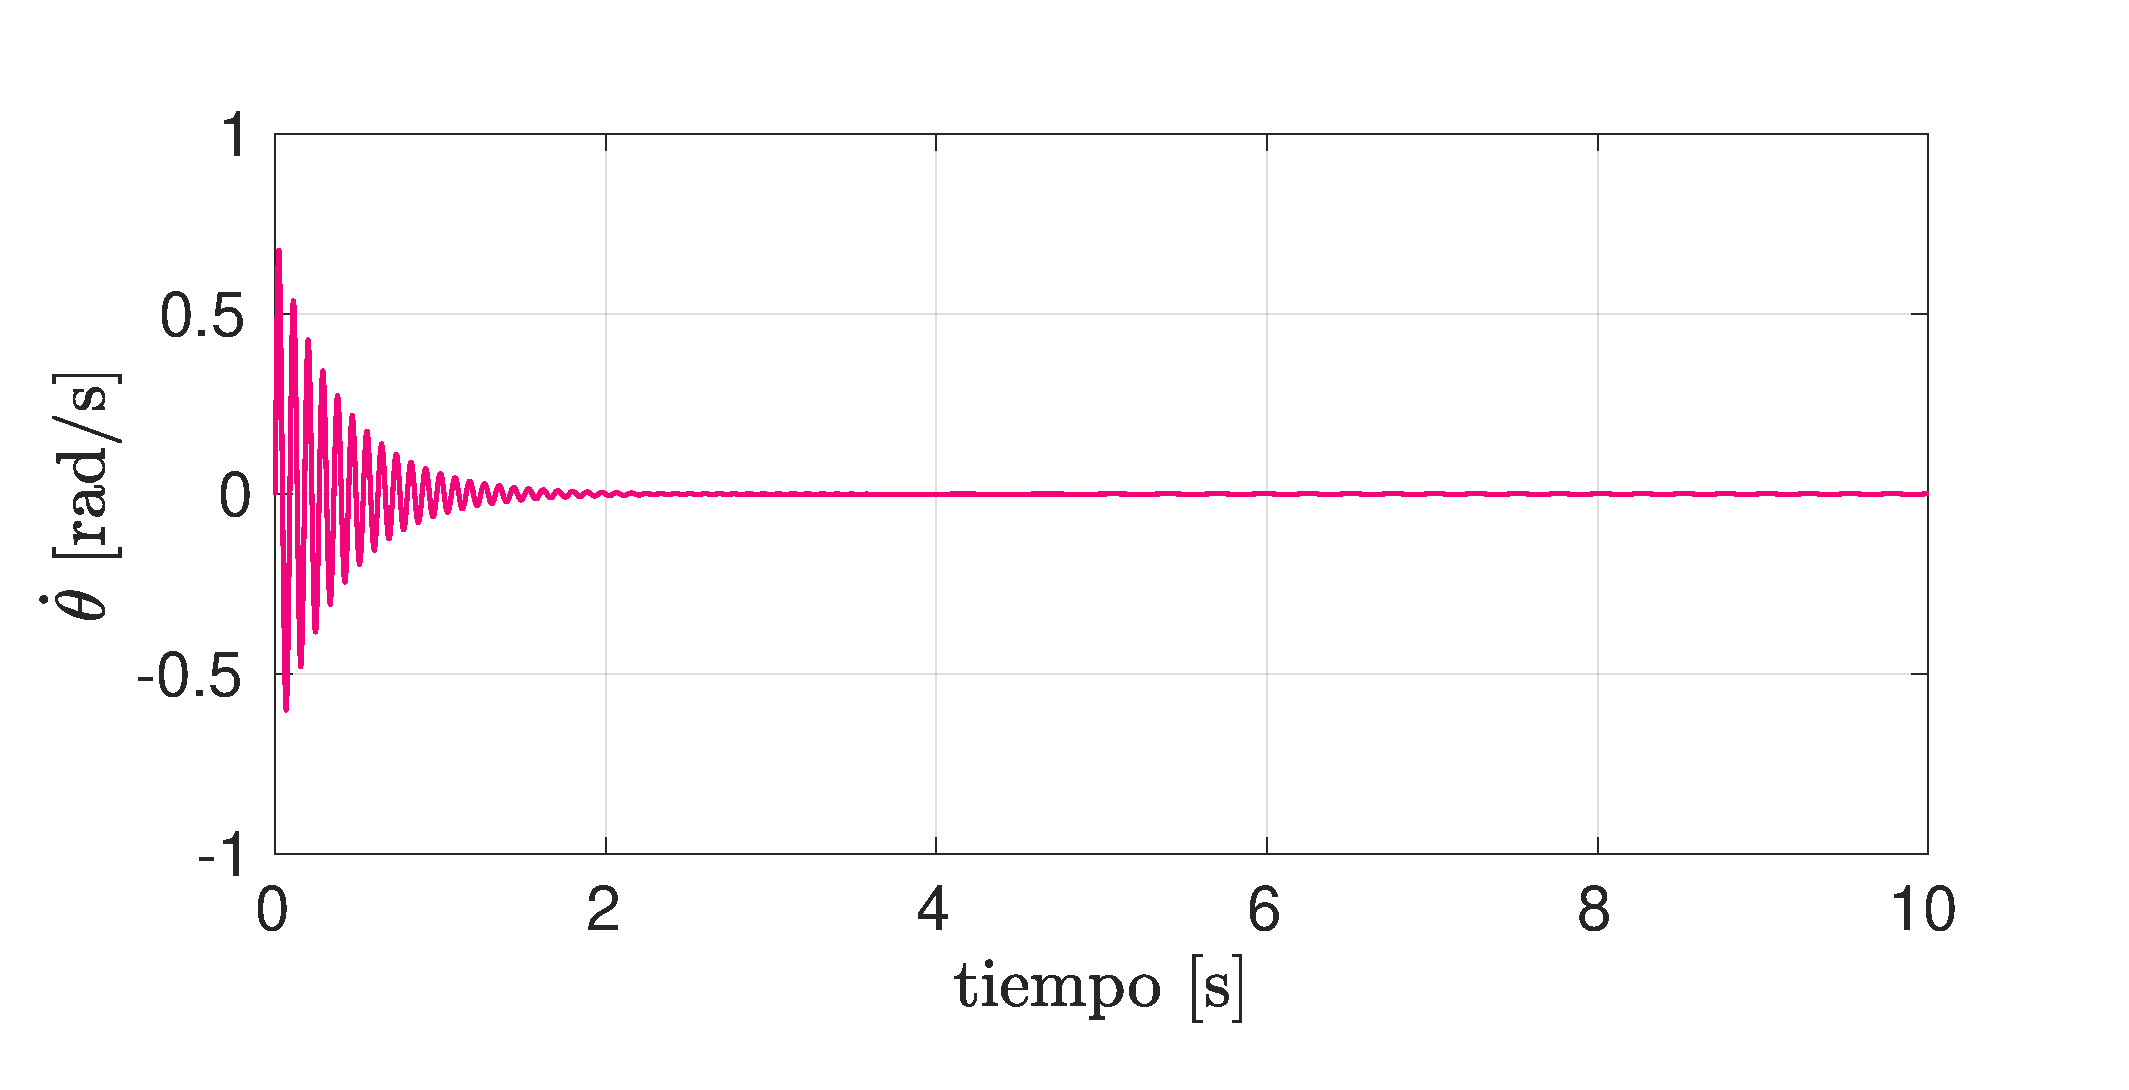
\includegraphics[width=1\linewidth]{Imagenes/tp_1.pdf}
%		\caption{}\label{fig:tp_1}
%	\end{subfigure}
%	\begin{subfigure}{1\linewidth}
%		\centering
%		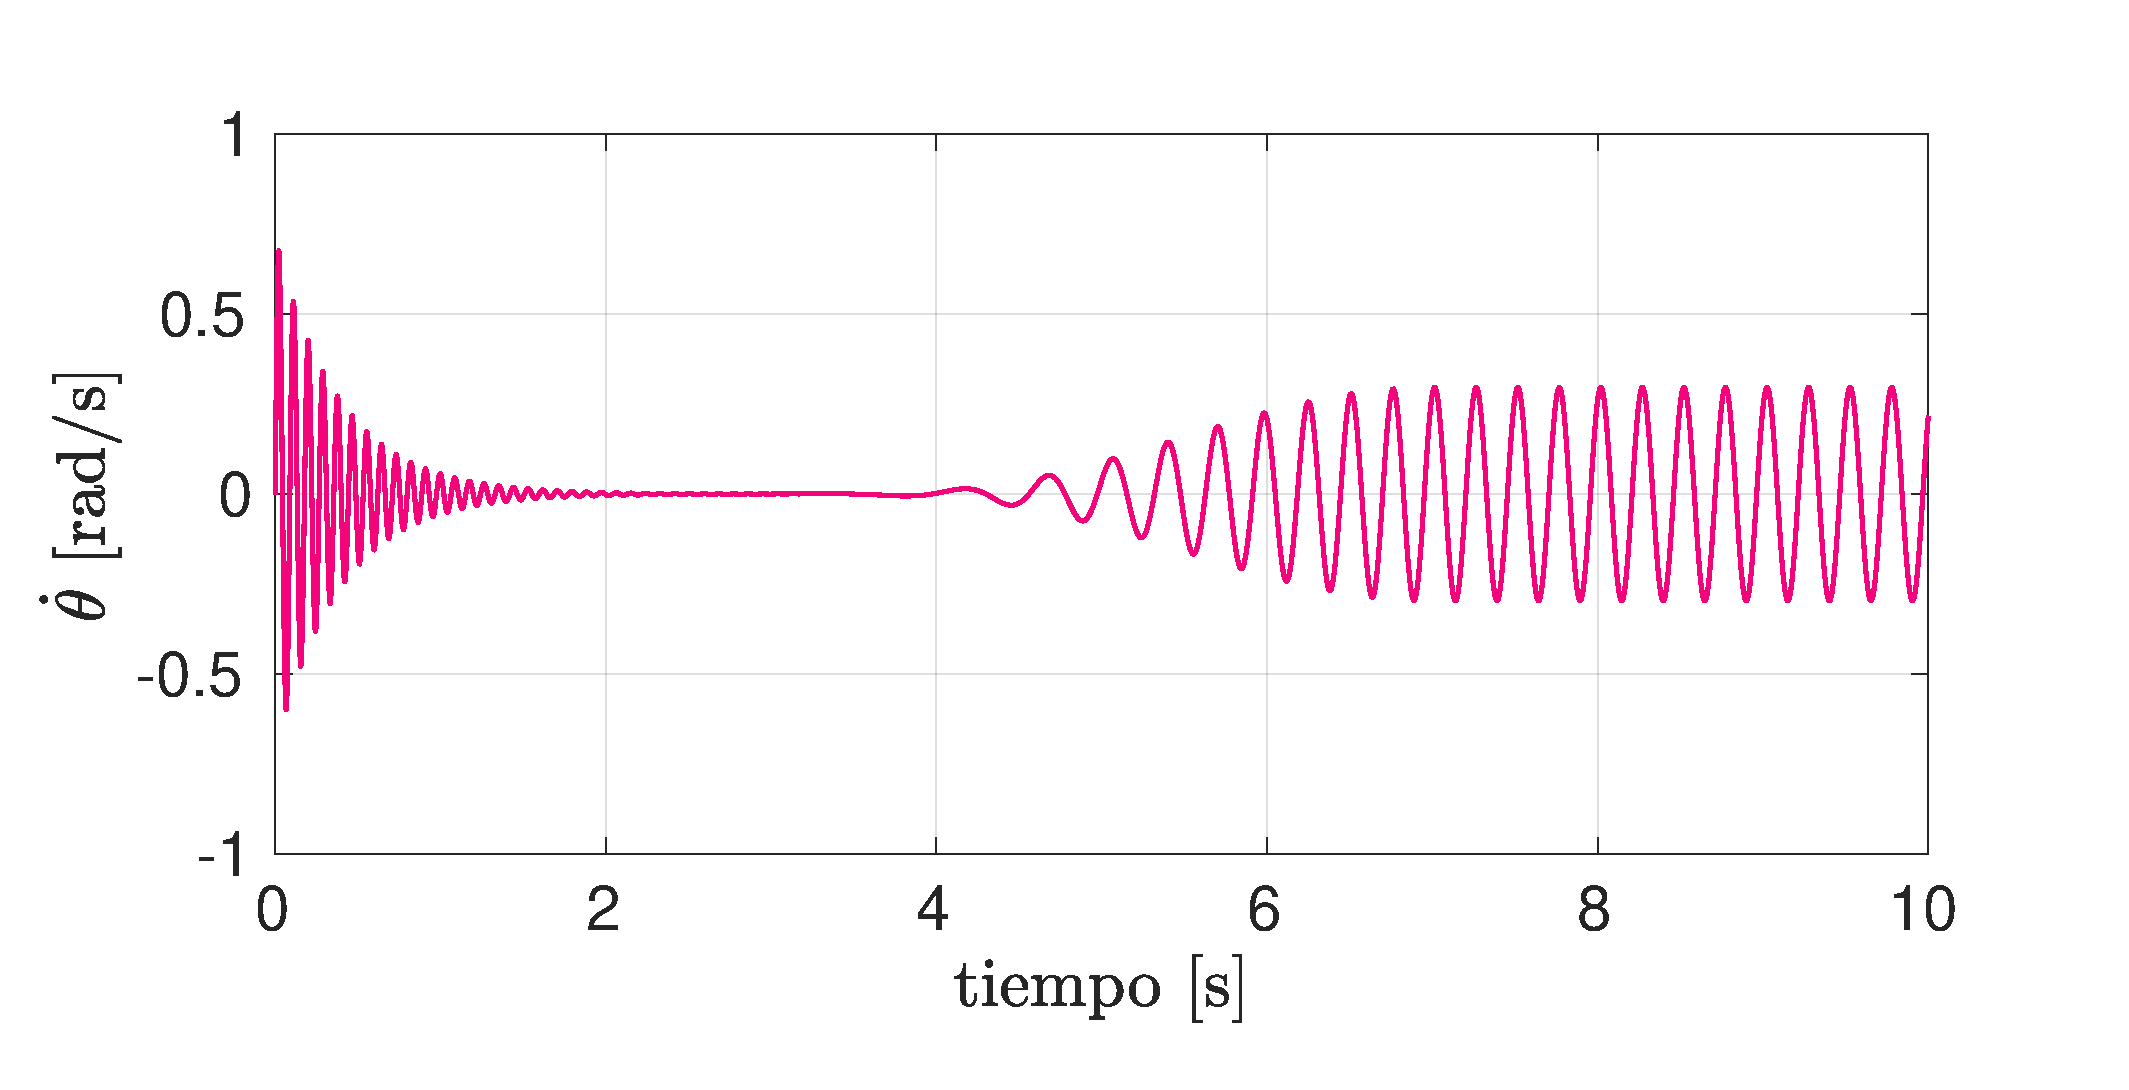
\includegraphics[width=1\linewidth]{Imagenes/tp_2.pdf}
%		\caption{}\label{fig:tp_2}
%	\end{subfigure}
%\par\bigskip
%\caption{sadfafssafdasf}
%\label{fig:velt_12}
%\end{figure}
 
\newpage
 
\subsection{Carga máxima y media para cada configuración} 

En la sección anterior, se mostraron los resultados y el comportamiento del modelo para una configuración en específico. En esta sección, a través del código de la sección \ref{sec:sol_gen}, se mostrarán los resultados de fuerza máxima y media para cada combinación de contrapesos expuesta en la tabla de carga. Al ordenar los resultados de la fuerza máxima con el mismo orden de la tabla de carga, es decir, respecto a $\Delta m$, se obtiene la curva que se muestra en la fig. \ref{fig:fmax_dm25}. La carga más baja, es decir, para la combinación n$^{\circ}$ 1 es de $F_{max,1} = 13.7102$ [N], mientras que la carga más alta de la combinación n$^{\circ}$ 201 es de $F_{max,201} = 296.9143$ [N].

\begin{figure}[h]
\centering
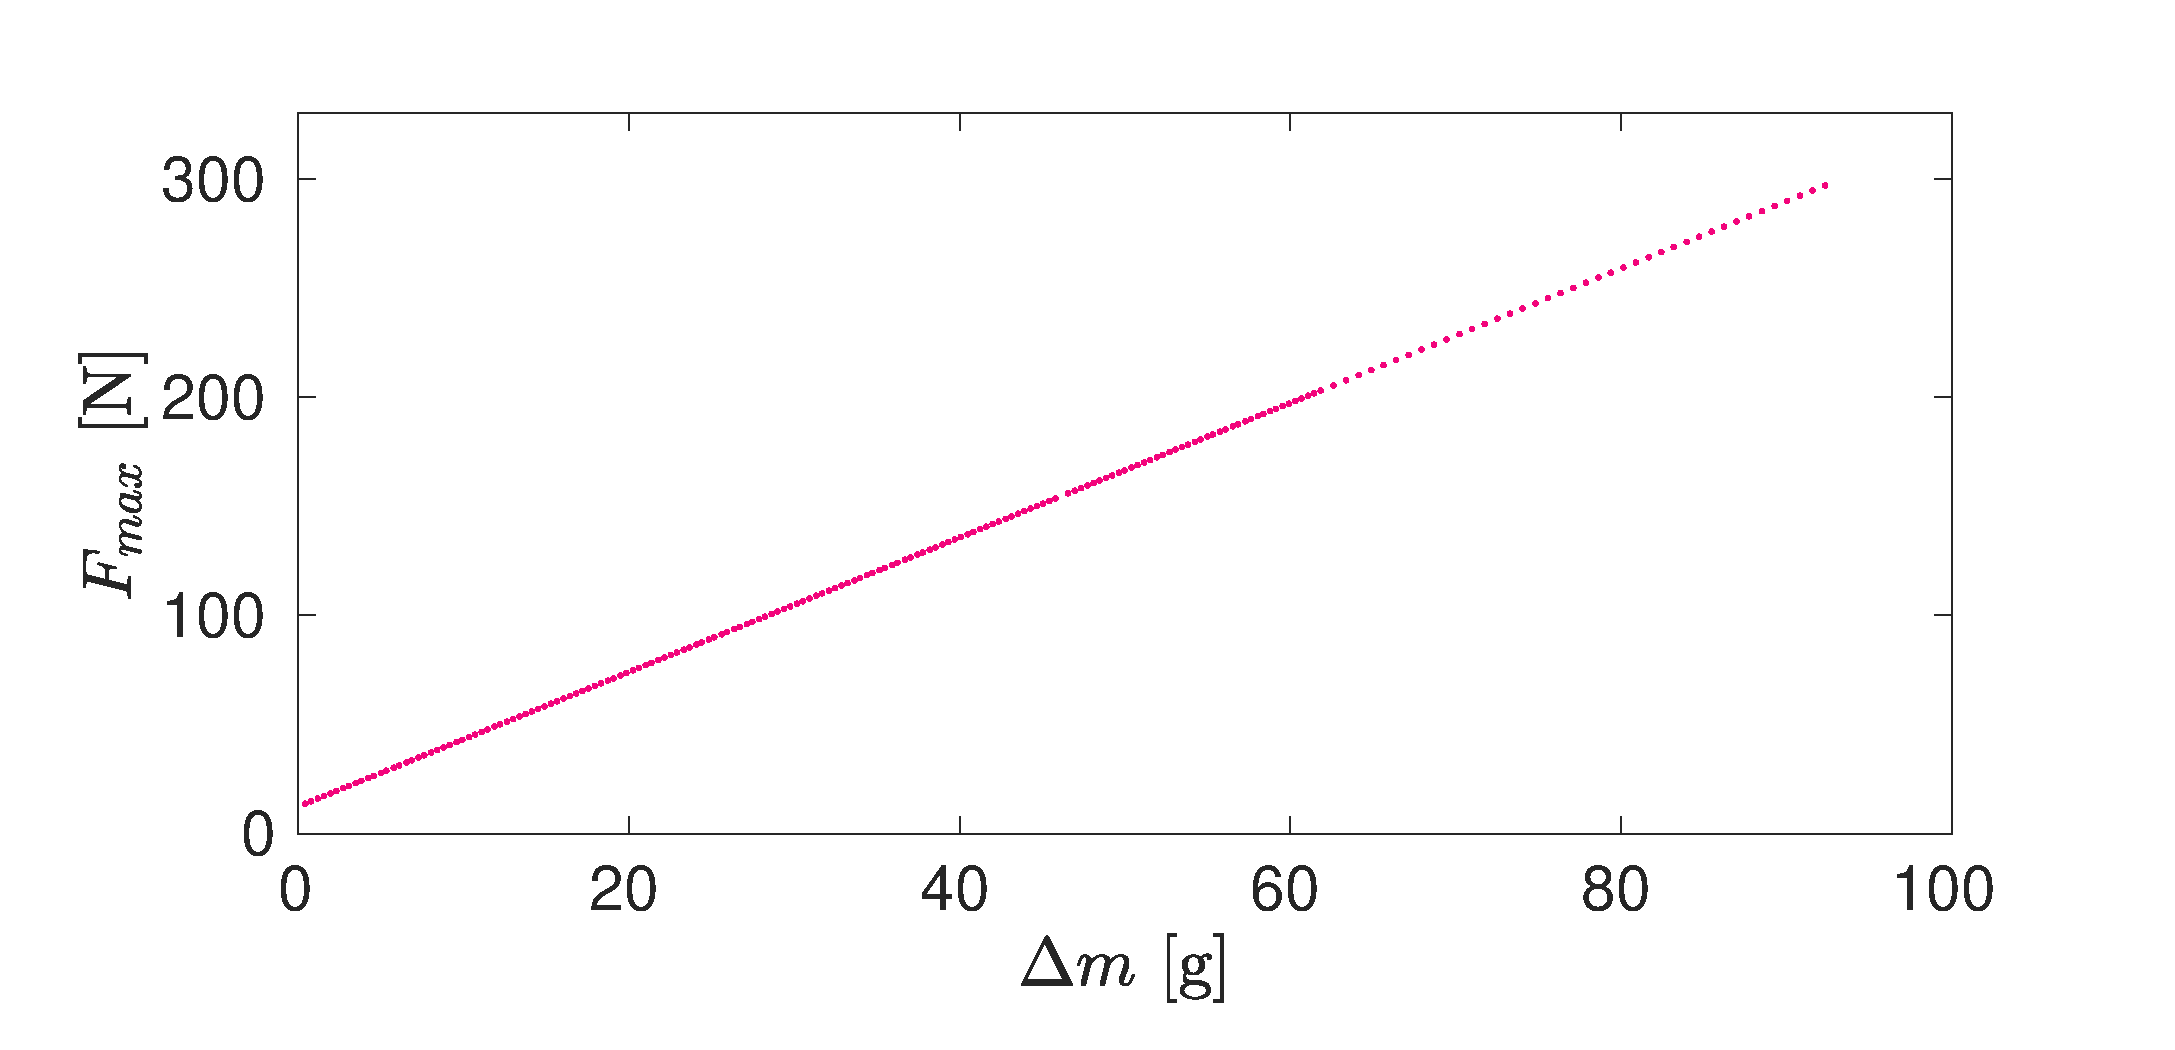
\includegraphics[width=\linewidth, trim={0cm 0cm 2cm 0cm},clip]{Imagenes/fmax_dm_25.pdf}
\caption{Distribución de la carga máxima $F_{max}$ versus la diferencia de masas $\Delta m$ de cada combinación de contrapesos, con $\omega_{max} =$ 1500 rpm. Resultados en el anexo \ref{sec:anexob2}}
\label{fig:fmax_dm25}
\end{figure}

A partir de la figura, se puede establecer que el modelo mantiene la relación entre la carga máxima $F_{max}$ y $\Delta m$, como lo hace la tabla de carga. En consecuencia, la carga máxima es función del desbalanceo existente en el disco rotatorio, por lo tanto, se puede definir la siguiente relación: 
\begin{equation}\label{eq:func_dm}
	F(t) = f(\Delta m)
\end{equation}

Por otro lado, la carga media permanece prácticamente constante, como se puede ver en la fig. \ref{fig:fm_dm}, siendo la diferencia máxima de $7\cdot10^{-4}$ [N] (fig \ref{fig:fm_dmsp}). Tomando en consideración que el orden de magnitud de las cargas máxima y alternantes está en el orden de $10^1$ y $10^2$, entonces se puede asumir que la carga media que sufrirá la probeta será constante y de una magnitud de $12.438$ [N]. 

\begin{figure}[H]
\centering
	\begin{subfigure}{1\linewidth}
		\centering
		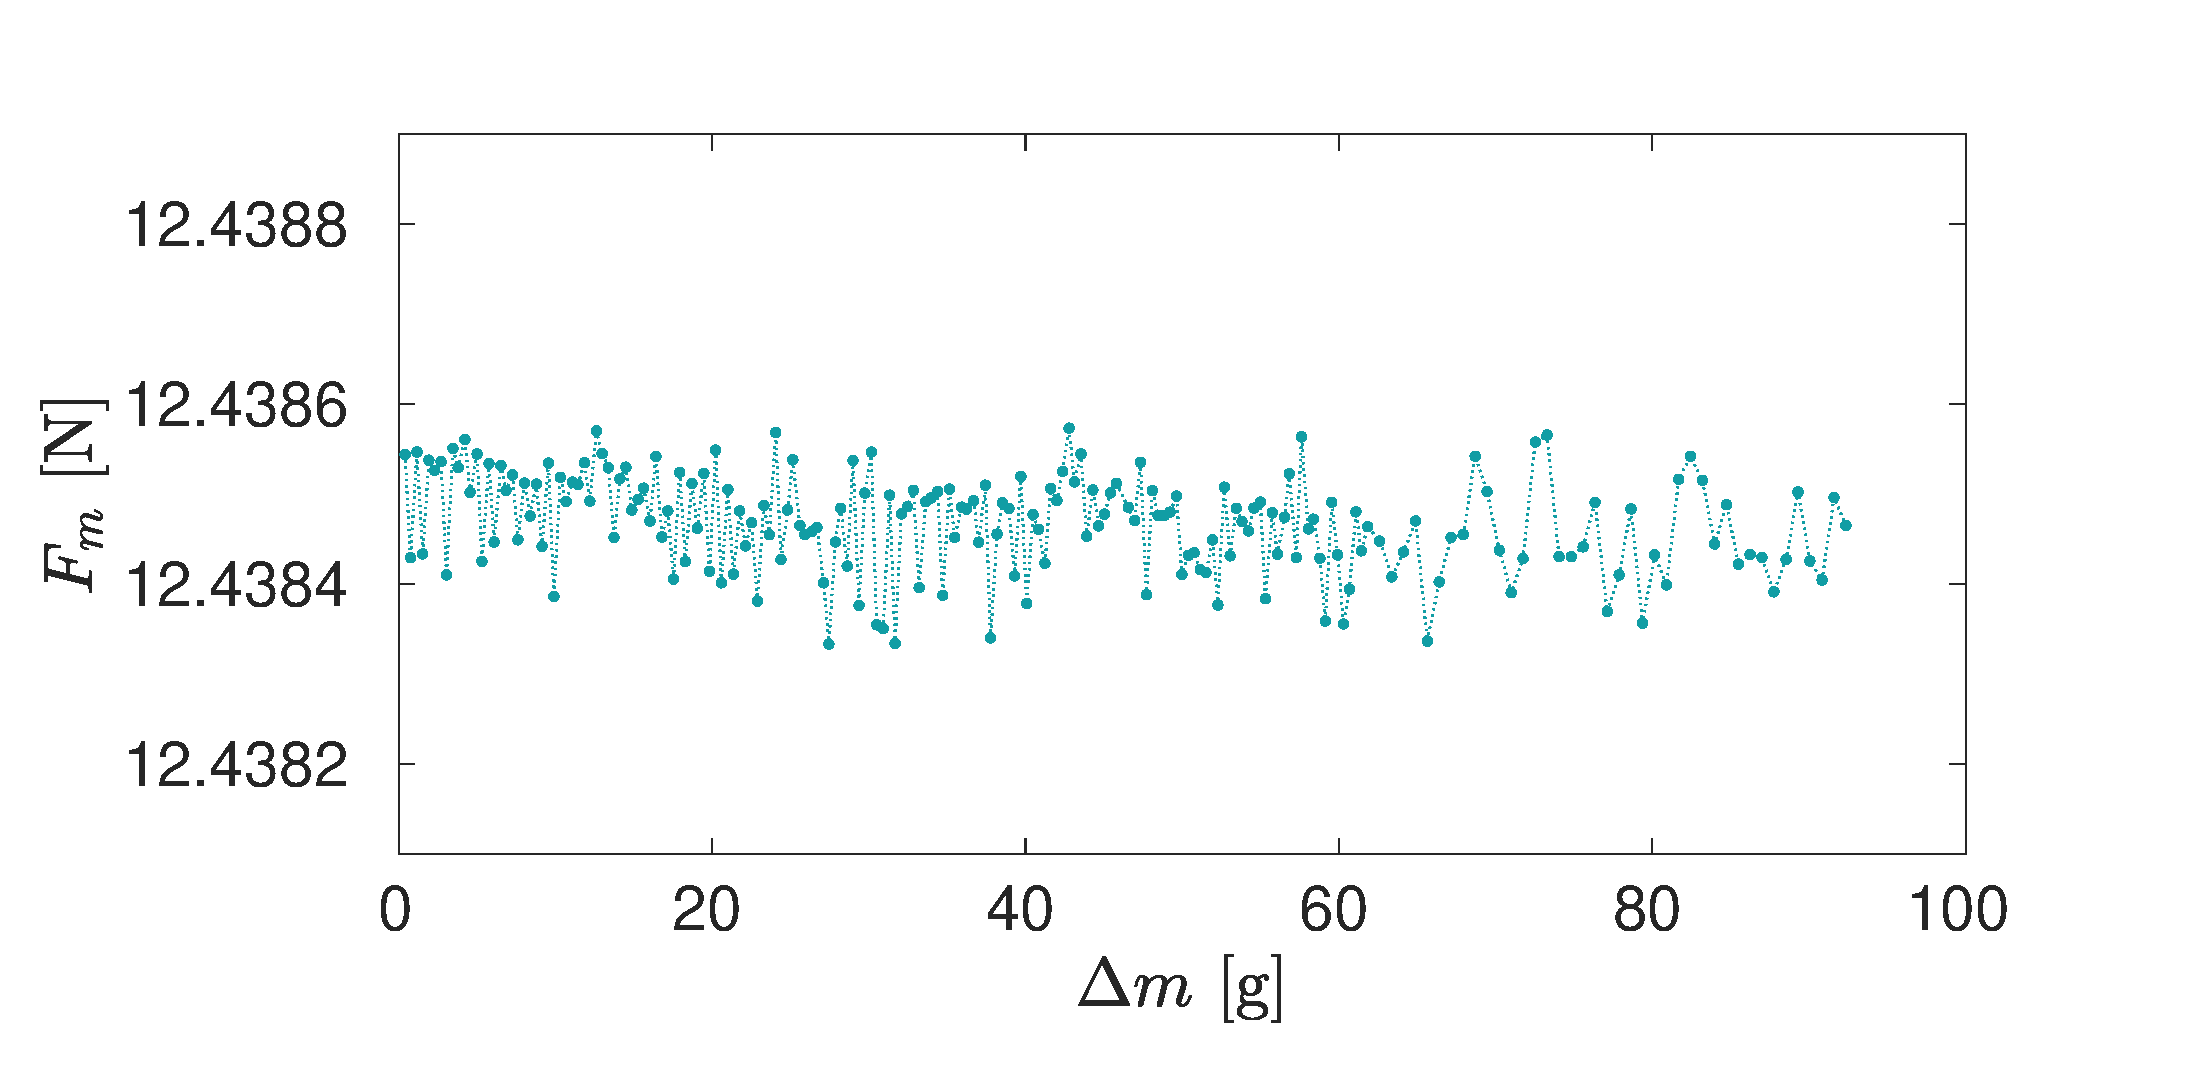
\includegraphics[width=1\linewidth]{Imagenes/fm_dm.pdf}
		\caption{Carga media de cada configuración de contrapesos.}\label{fig:fm_dm}
	\end{subfigure}
	\begin{subfigure}{1\linewidth}
		\centering
		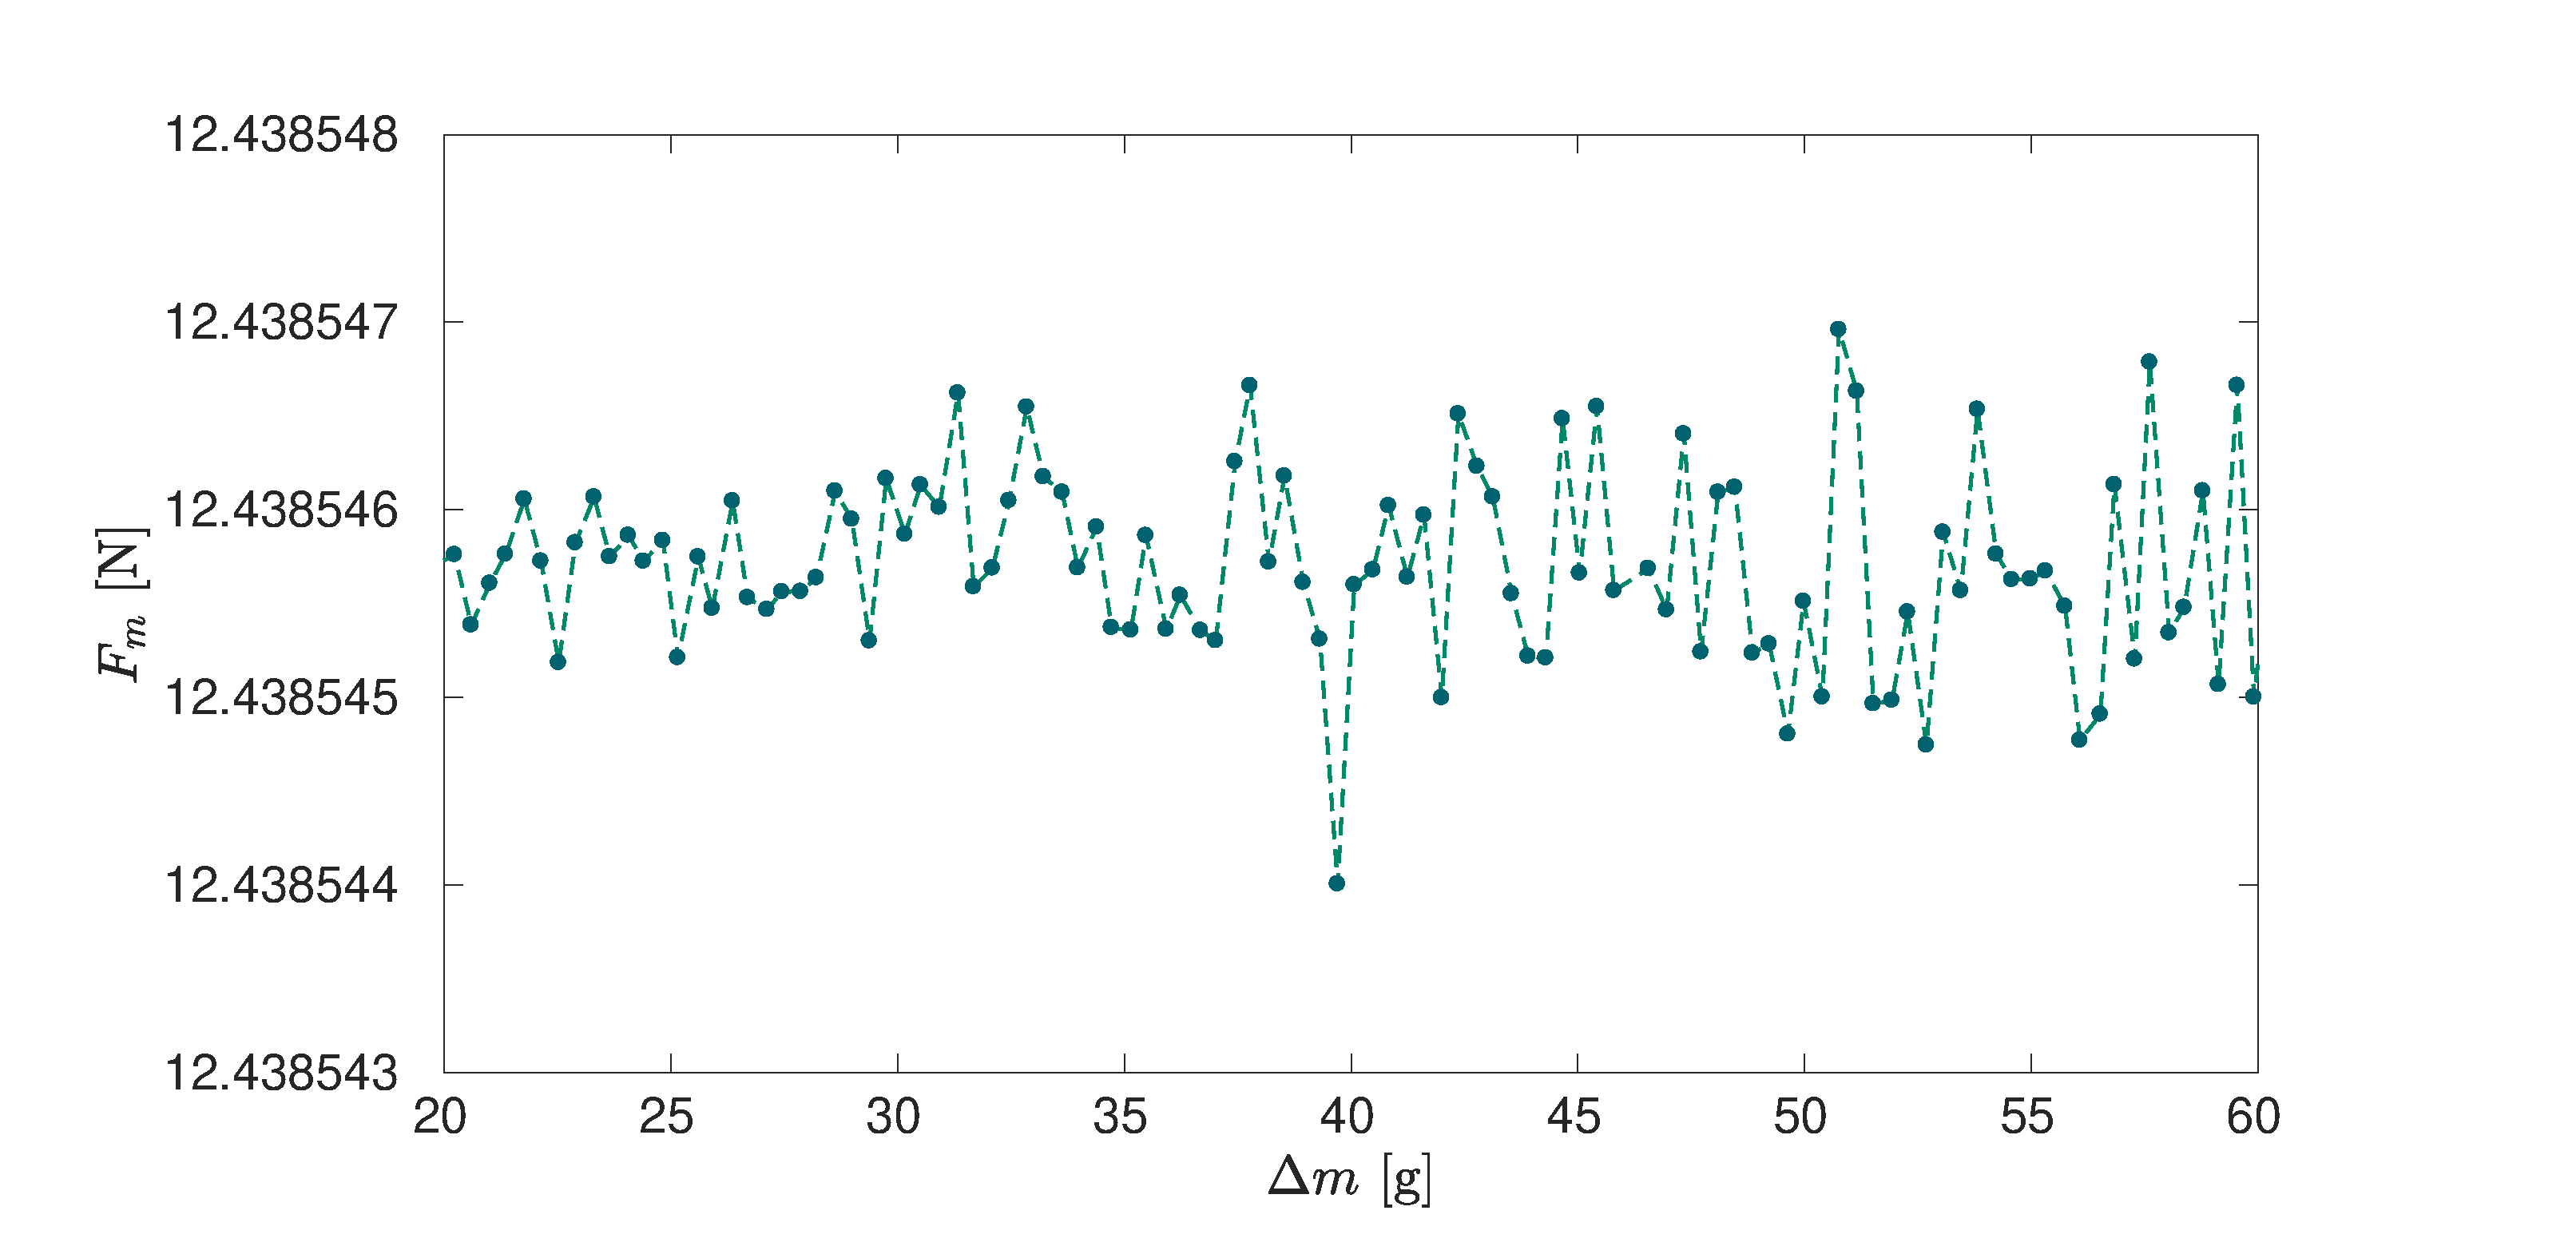
\includegraphics[width=1\linewidth]{Imagenes/fm_dmsp.pdf}
		\caption{Acercamiento a la curva entre los 12.4380 [N] y 12.4390 [N] de $F_m$. }\label{fig:fm_dmsp}
	\end{subfigure}
\par\bigskip
\caption{Distribución de la carga media ($F_m$) para las distintas configuraciones de contrapeso.}
\label{fig:velt_12}
\end{figure}

\newpage

\subsection{Influencia de la velocidad de rotación del disco desbalanceado sobre la carga en la probeta}

De manera análoga, se puede estudiar la influencia de la velocidad de giro máxima del disco desbalanceado sobre el movimiento del sistema. Las figuras en \ref{fig:f_w520}, muestran $F(t)$ para dos velocidad distintas, $\omega_{max,a} = 250$ rpm y $\omega_{max,b}=1000$ rpm. 

Ambas gráficas muestran no sólo como la frecuencia de la oscilación es menor en la figura \ref{fig:f_w250} respecto a \ref{fig:f_w1000}, como es esperable, sino que también la fuerza sobre la probeta aumenta en la medida que la velocidad de rotación del disco es mayor. Esta información, junto a la expuesta en la sección anterior, muestra que el modelo responde a las distintas variables de la fuerza producida por el disco $F_d(t)$. 

\begin{figure}[p]
\centering
	\begin{subfigure}{1\linewidth}
		\centering
		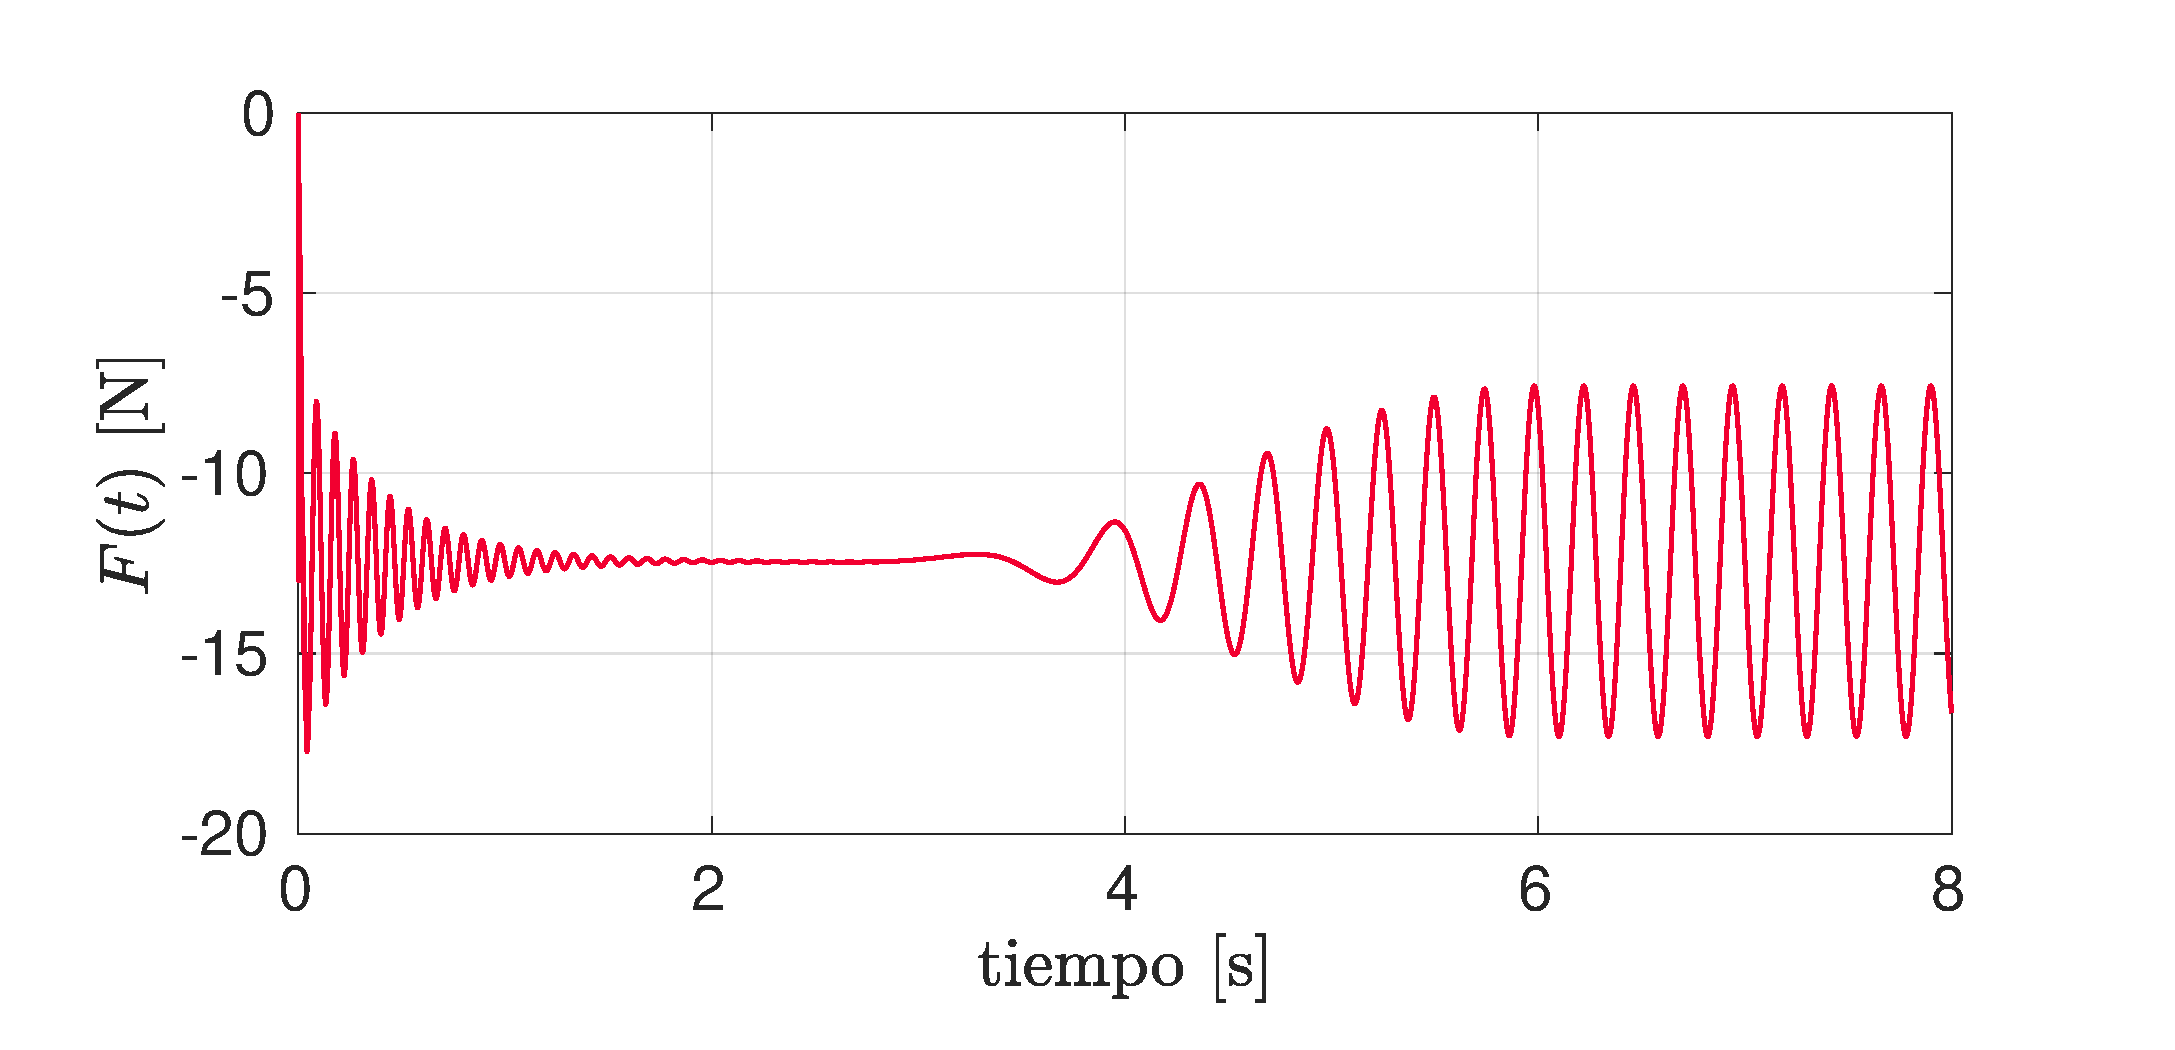
\includegraphics[width=\linewidth, trim={0cm 0cm 2cm 0cm},clip]{Imagenes/f_w250.pdf}
		\caption{Fuerza sobre la probeta a través del tiempo a $\,\omega_{max}=250$ rpm.}
		\label{fig:f_w250}
	\end{subfigure}
	\begin{subfigure}{1\linewidth}
		\centering
		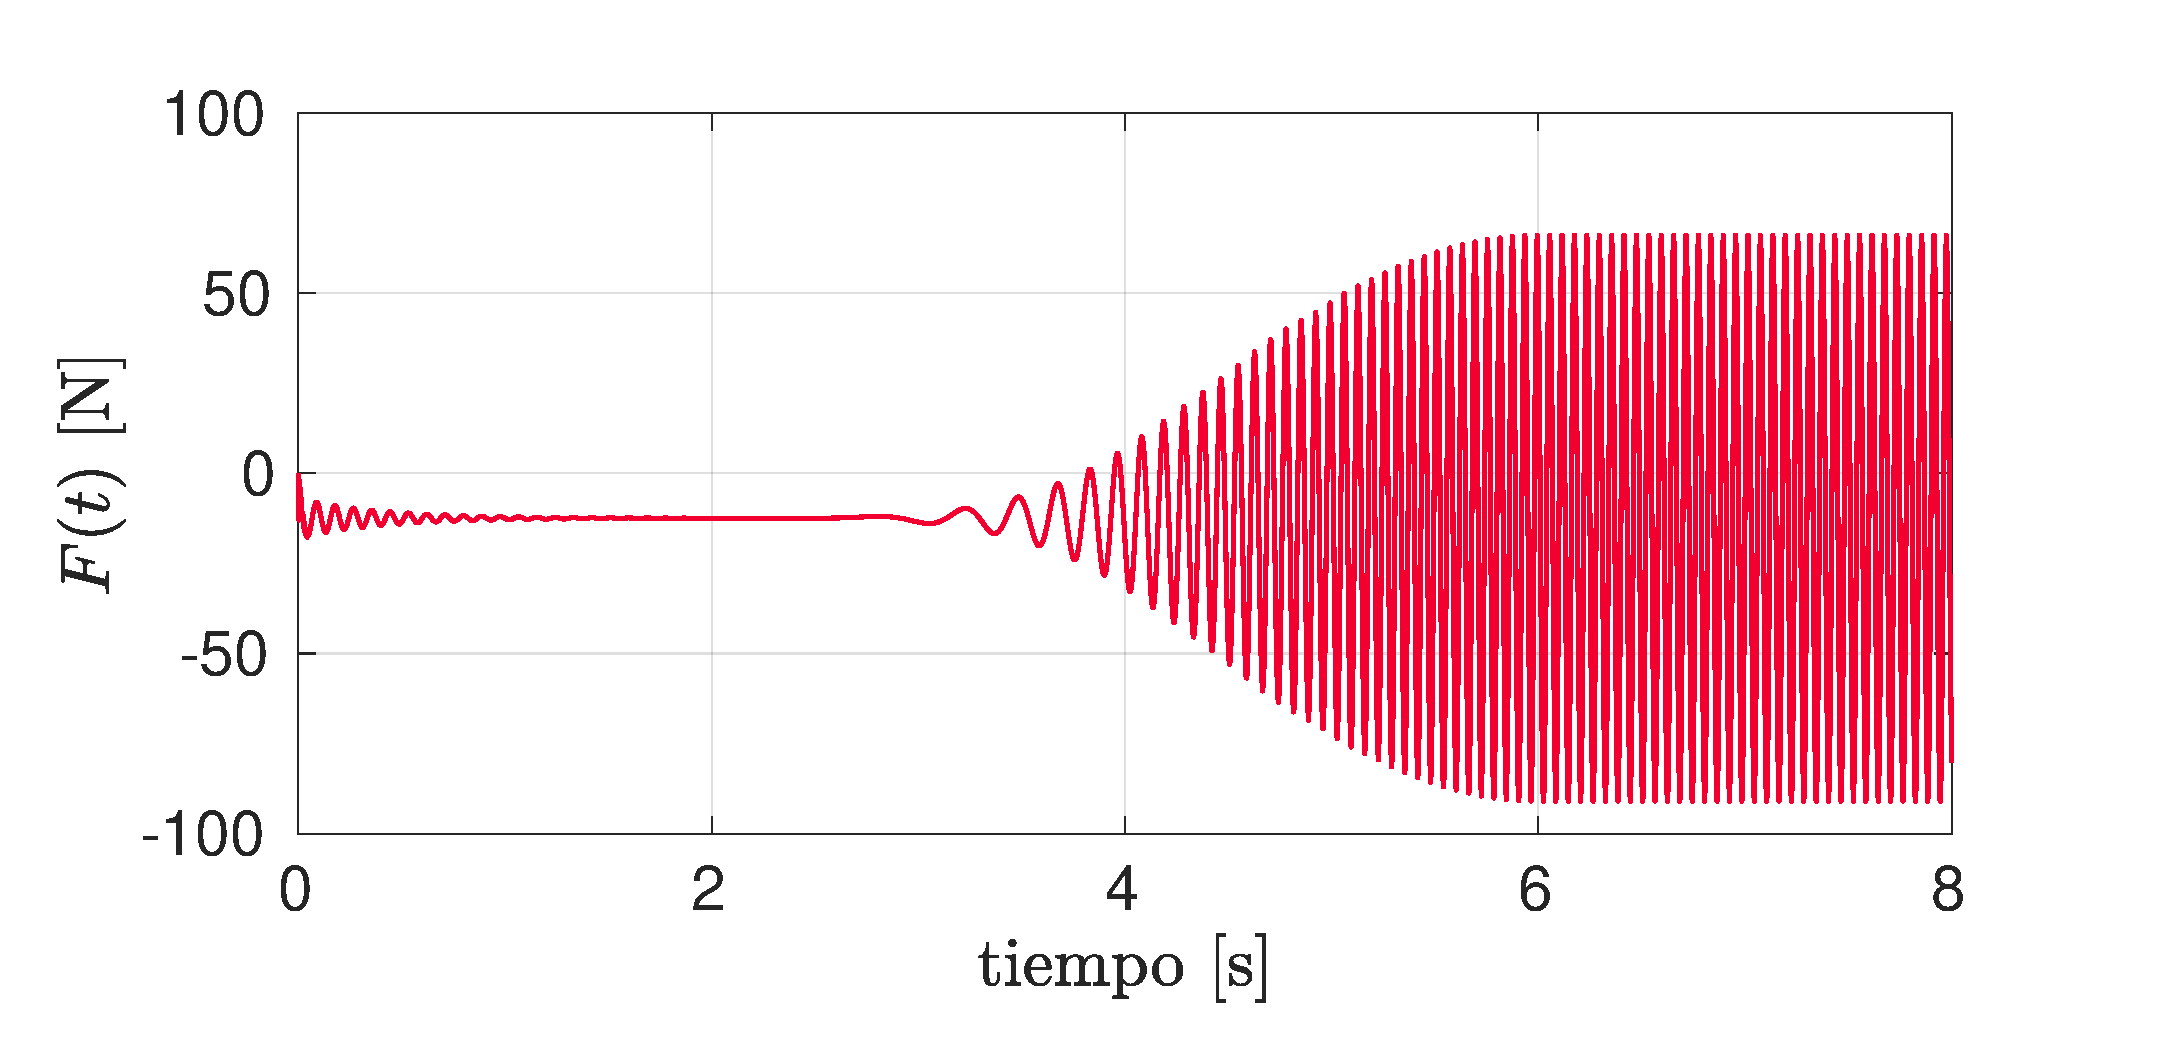
\includegraphics[width=\linewidth, trim={0cm 0cm 2cm 0cm},clip]{Imagenes/f_w1000.pdf}
		\caption{Fuerza sobre la probeta a través del tiempo a $\omega_{max}=1000$ rpm.}
		\label{fig:f_w1000}
	\end{subfigure}
\caption{Comparación de la fuerza aplicada sobre la probeta $F(t)$, para una carga de $\Delta m = 57.6137$ g, a dos velocidades angulares $\omega_{max}$ distintas.}
\label{fig:f_w520}
\end{figure}

A continuación, es posible comparar la fuerza máxima de cada combinación de contrapesos para distintas velocidades angulares $\omega_{max}$. Aquí se confirma el comportamiento descrito anteriormente para una configuración específica, pero de manera general para cada una de las 201 combinaciones existentes, como se puede ver en la fig. \ref{fig:fmax_dm}. Al realizarse el conjunto de ensayos de fatiga para crear la curva $S$-$N$ a una velocidad fija, pero variando los contrapesos, se puede definir que la fuerza sobre la probeta como:
\begin{equation}\label{eq:func_psiomega}
	F(t) = f(\Delta m,\: \omega_{max})
\end{equation}

A partir de la fig. \ref{fig:fmax_dm}, se puede concluir que para cada velocidad de rotación del disco $\omega$ existe una relación lineal entre la carga máxima $F_{max}$ y $\Delta m$, frente a lo cual se puede asociar una pendiente $\eta$. Esta aumenta a medida que $\omega$ se incrementa, por lo tanto al gráficar ambos parámetros se puede ver como la pendiente crece de manera cuadrática respecto al aumento de la velocidad angular (fig. \ref{fig:eta_w}), en consecuencia se puede ajustar una curva al comportamiento de la pendiente $\eta$, dada por la siguiente ecuación cuadrática:
\begin{equation}
	\eta = 0.0014\cdot \omega^2 - 0.0092\cdot \omega + 0.75
\end{equation}
Siendo $\eta$ la pendiente y $\omega$ la velocidad angular. Esto nos permite poder predecir completamente el comportamiento de la máquina de fatiga, al conocer su relación entre la velocidad del motor ($\omega$), el desbalanceo en el disco ($\Delta m$), la carga media ($F_m$) y la carga máxima ($F_{max}$).

\begin{sidewaysfigure}[p]
\centering
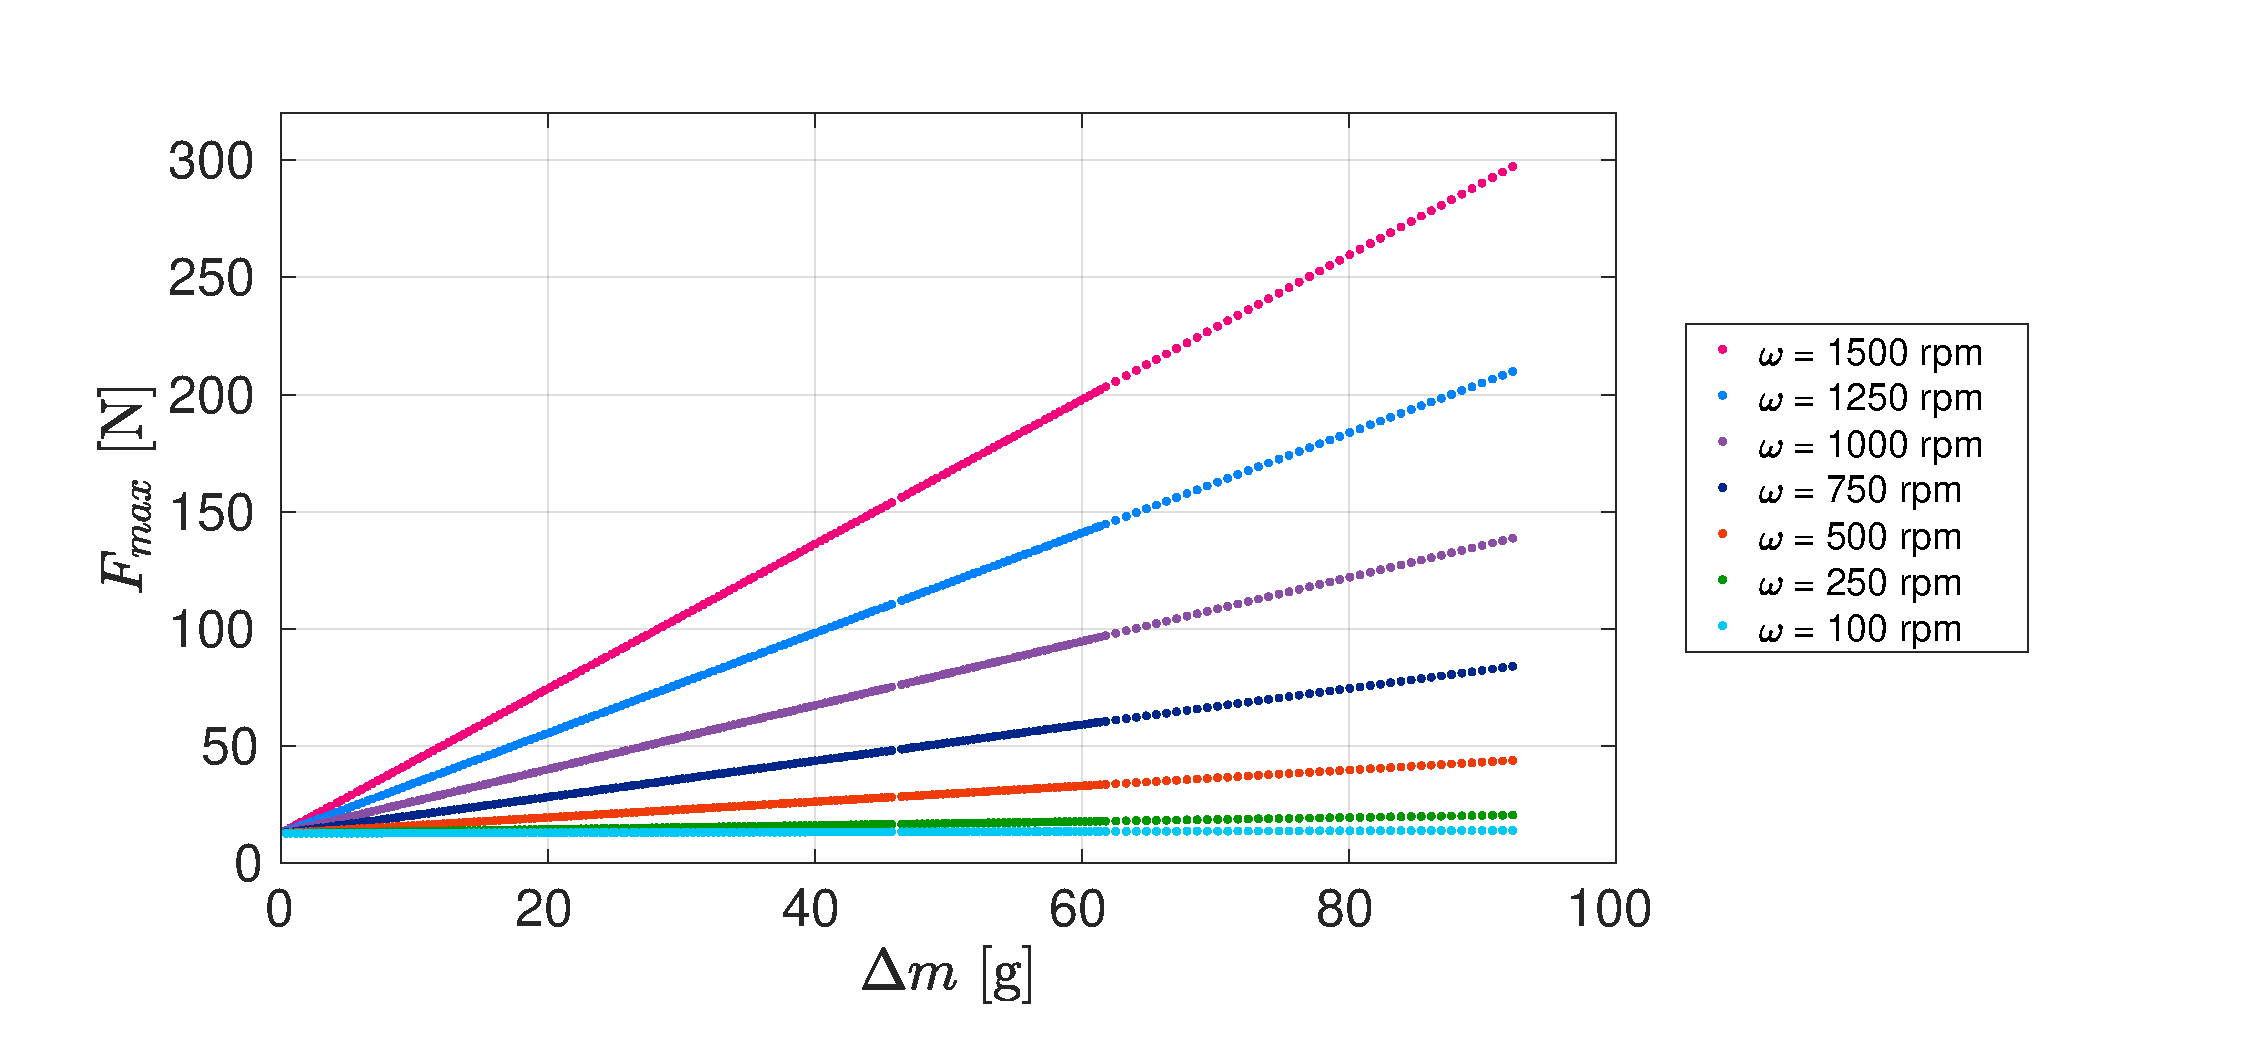
\includegraphics[width=1\linewidth, trim={1cm 0cm 3cm 1cm}, clip]{Imagenes/fmax_dm.pdf}
\caption{Curvas de cada combinación de contrapesos para distintas velocidades angulares $\; \omega_{max}$.}
\label{fig:fmax_dm}
\end{sidewaysfigure}

\begin{figure}[h]
\centering
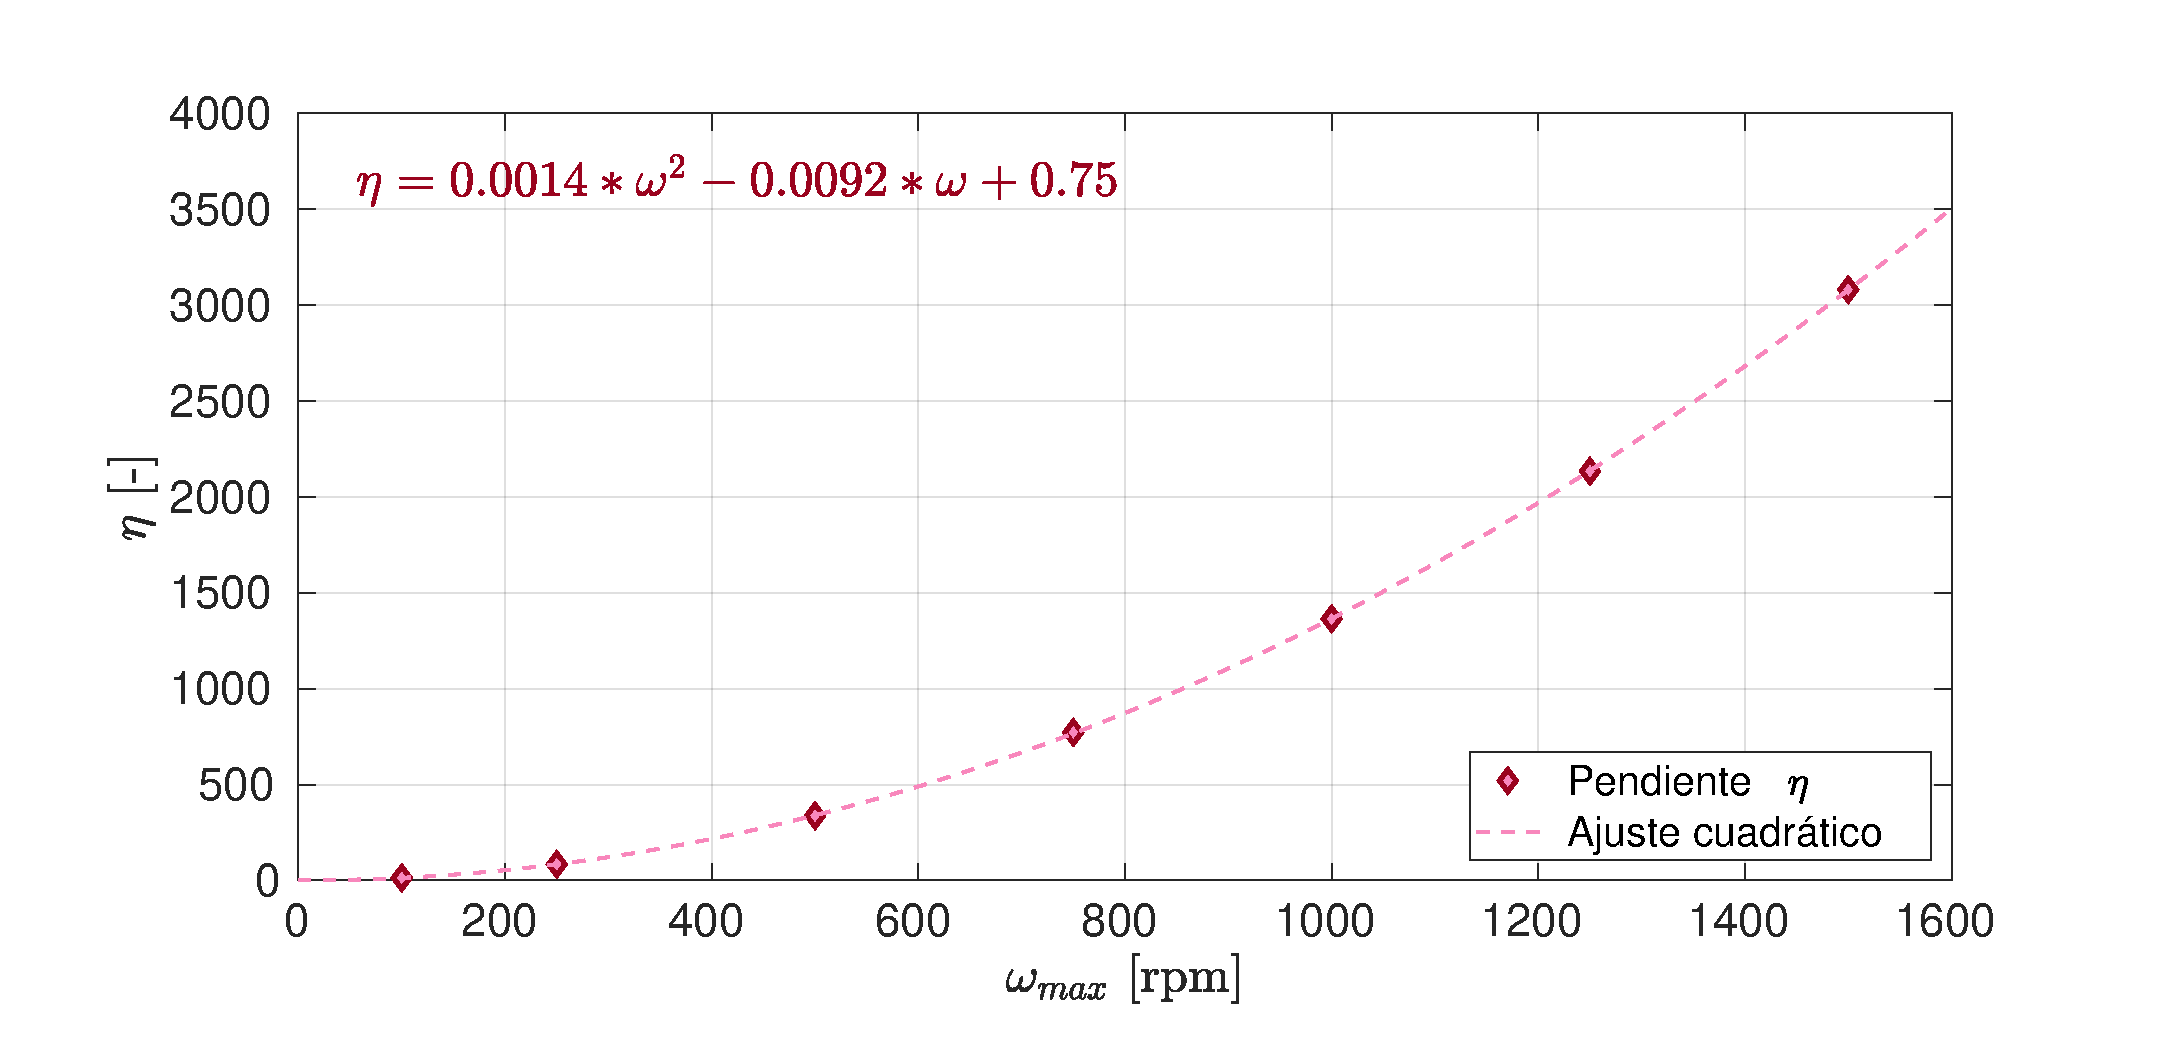
\includegraphics[width=1\linewidth, trim={1cm 0cm 2cm 1cm}, clip]{Imagenes/eta_w.pdf}
\caption{Curva de la pendiente $\eta$ para cada velocidad $\omega$ del disco desbalanceado.}
\label{fig:eta_w}
\end{figure}

\newpage

Como consecuencia de los resultados que se obtuvieron del modelo, estos se deben comparar con la información existente en la tabla de cargas. Para esto, es necesario conocer los esfuerzos asociados a cada combinación de contrapesos, de la misma forma que lo hace la tabla actual. Por consiguiente, se realizará una simulación de las cargas que se obtuvieron en este análisis, al aplicarlas sobre la probeta, en la siguiente sección. Cabe destacar que estos resultados, basados en los desplazamientos del brazo de carga, deben ser corroborados empíricamente a posteriori, como parte del trabajo futuro. 

\newpage

\section{Simulación de carga máxima}

Al tomar los datos de las cargas máximas obtenidas a través del modelo e ingresarlas al software de elementos finitos ANSYS, se obtienen los esfuerzos que sufre la probeta para cada carga. En primer lugar, los valores de carga se pasan a presión para ser aplicado sobre una de las caras de la probeta, utilizando la ecuación \ref{eq:p_max}. La fig. \ref{fig:fmax_step}, muestra las 201 cargas aplicadas a lo largo de la simulación. 

\begin{figure}[h]
\centering
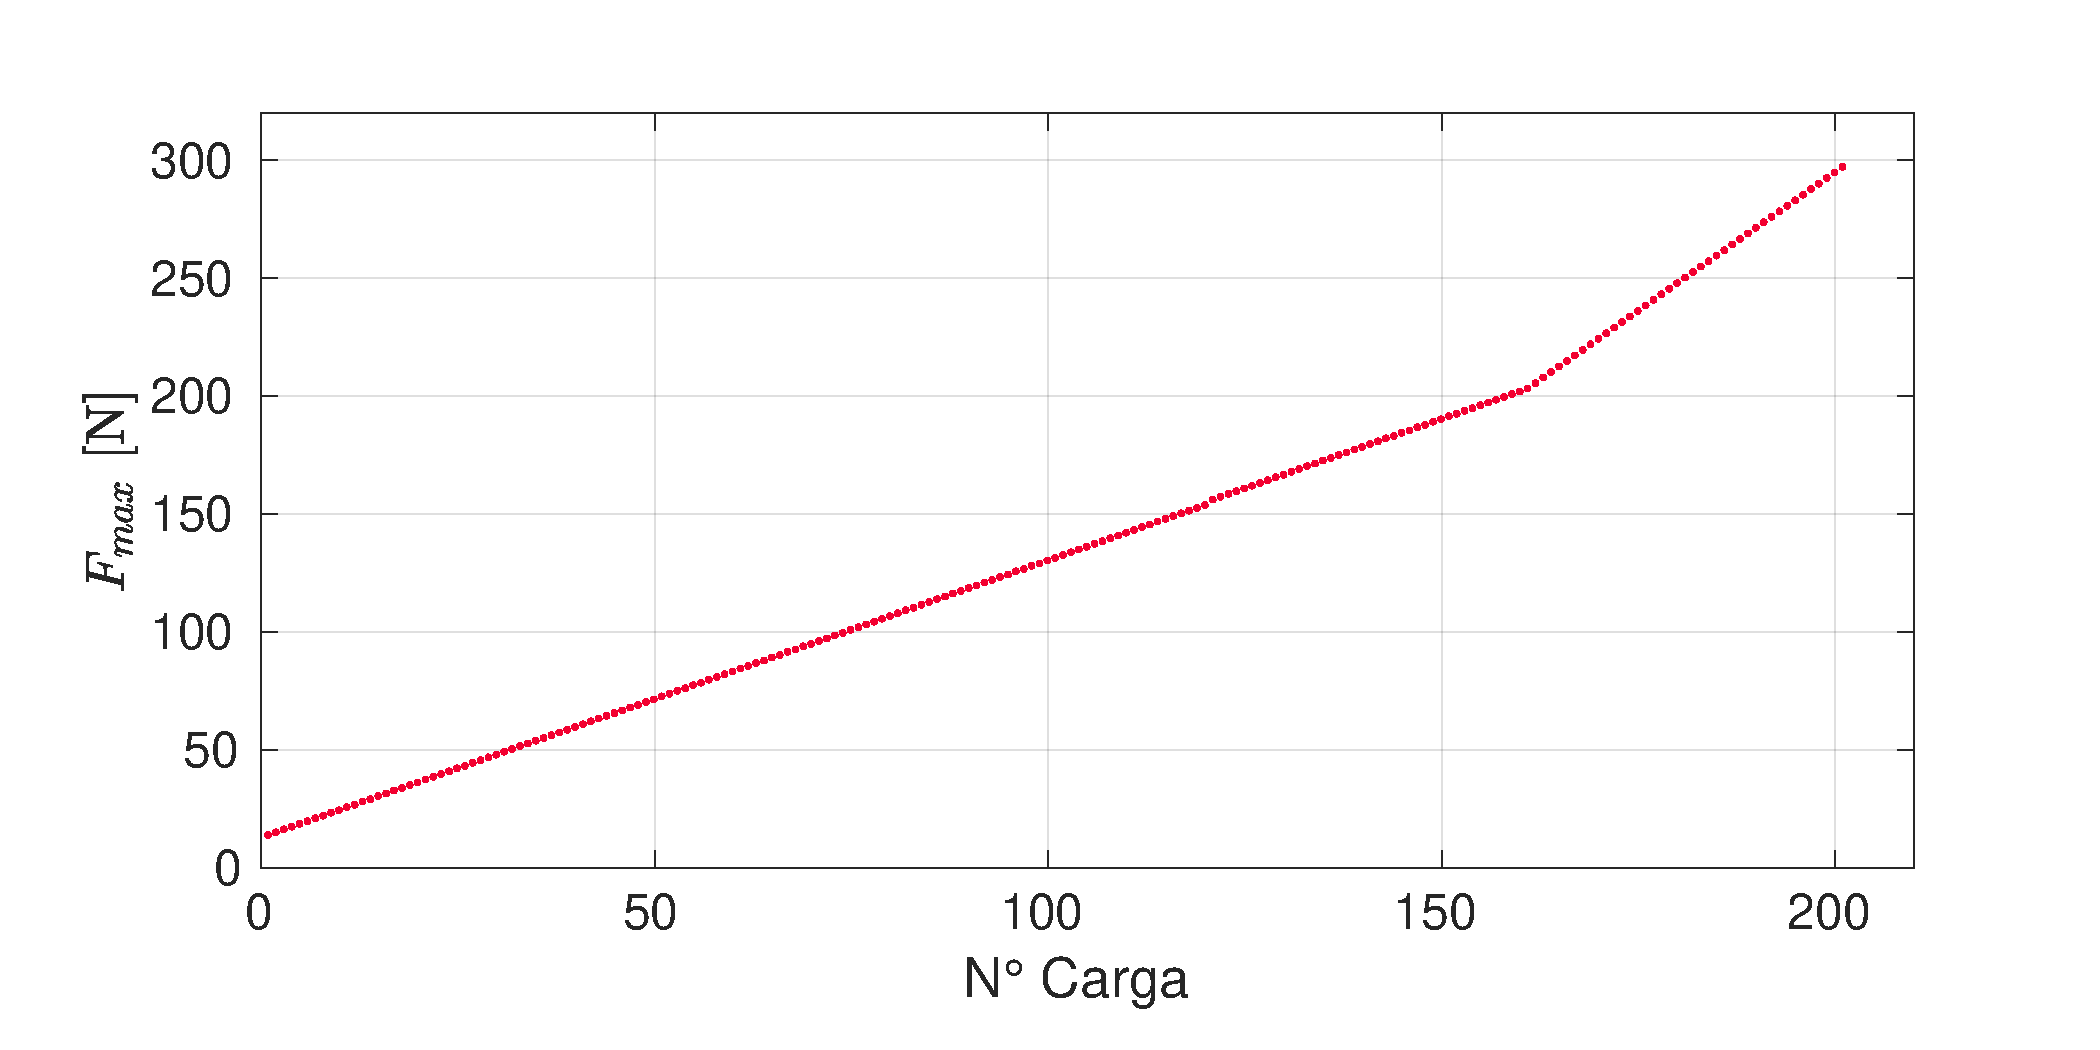
\includegraphics[width=1\linewidth, trim={1cm 0cm 1cm 0cm}, clip]{Imagenes/fmax_step.pdf}
\caption{Curva de las 201 cargas aplicadas sobre la probeta. Tabla en anexo \ref{sec:anexob2}}
\label{fig:fmax_step}
\end{figure}

Al ver los esfuerzos generales a los que está sometida la probeta, se identifica que la zona más afectada es la intermedia, concentrándose justo en la mitad de la probeta, como se ve en las figuras \ref{fig:r_lat} y \ref{fig:r_iso}. Al realizar un corte transversal en la mitad de la probeta (fig. \ref{fig:rcorte_iso}) se pueden apreciar más claramente la distribución de los esfuerzos equivalentes en la zona intermedia, concentrandose fuertemente en la zona inferior y superior de la cara transversal. La figura \ref{fig:rcorte} muestra directamente la cara sometida a la carga máxima y su distribución de esfuerzos, donde además, se puede ver que la zona cercana al eje neutro tiene esfuerzos menores a los que se encuentran más lejos de este. Esta información es posible verla directamente en el comportamiento que tienen los elementos  $P$, $Q$ y $R$ (ver fig. \ref{fig:diag_pqr2}).

\begin{figure}[p]
\centering
	\begin{subfigure}{0.8\linewidth}
		\centering
		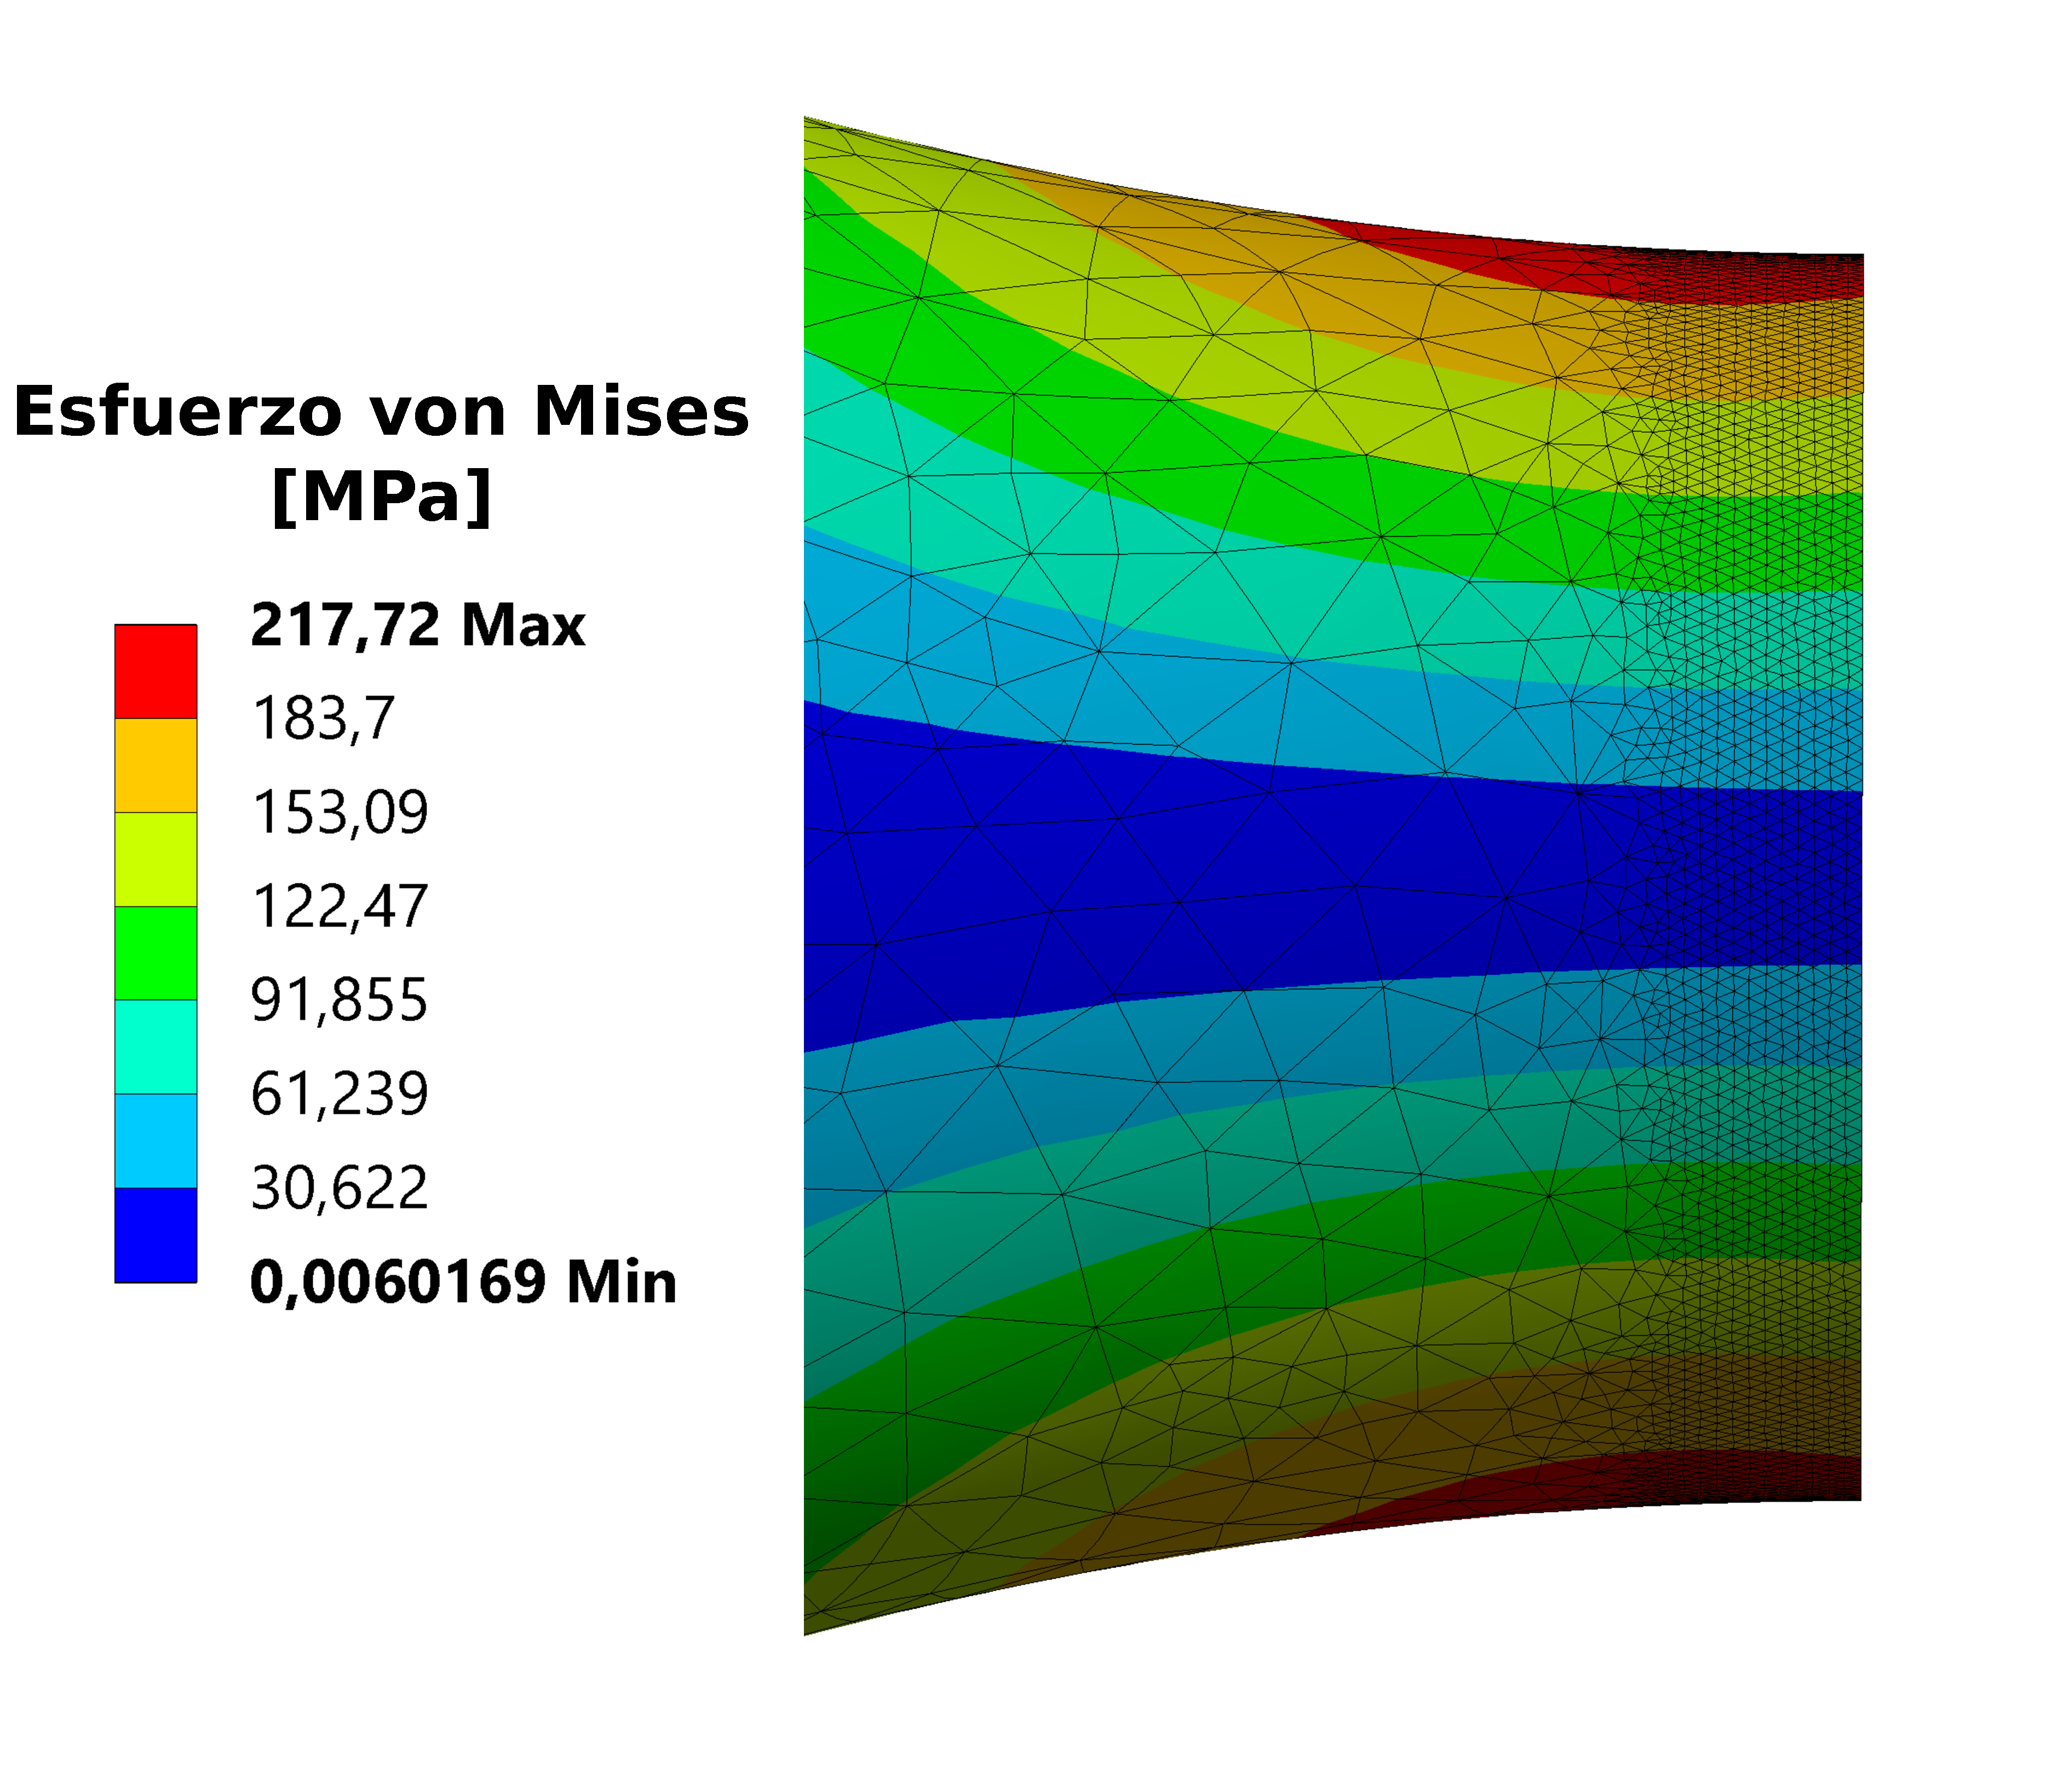
\includegraphics[width=0.9\linewidth]{Imagenes/esfvm_lat.pdf}
		\caption{Vista lateral de la zona intermedia.}
		\label{fig:corte_lat201}
	\end{subfigure}
	\begin{subfigure}{0.9\linewidth}
		\centering
		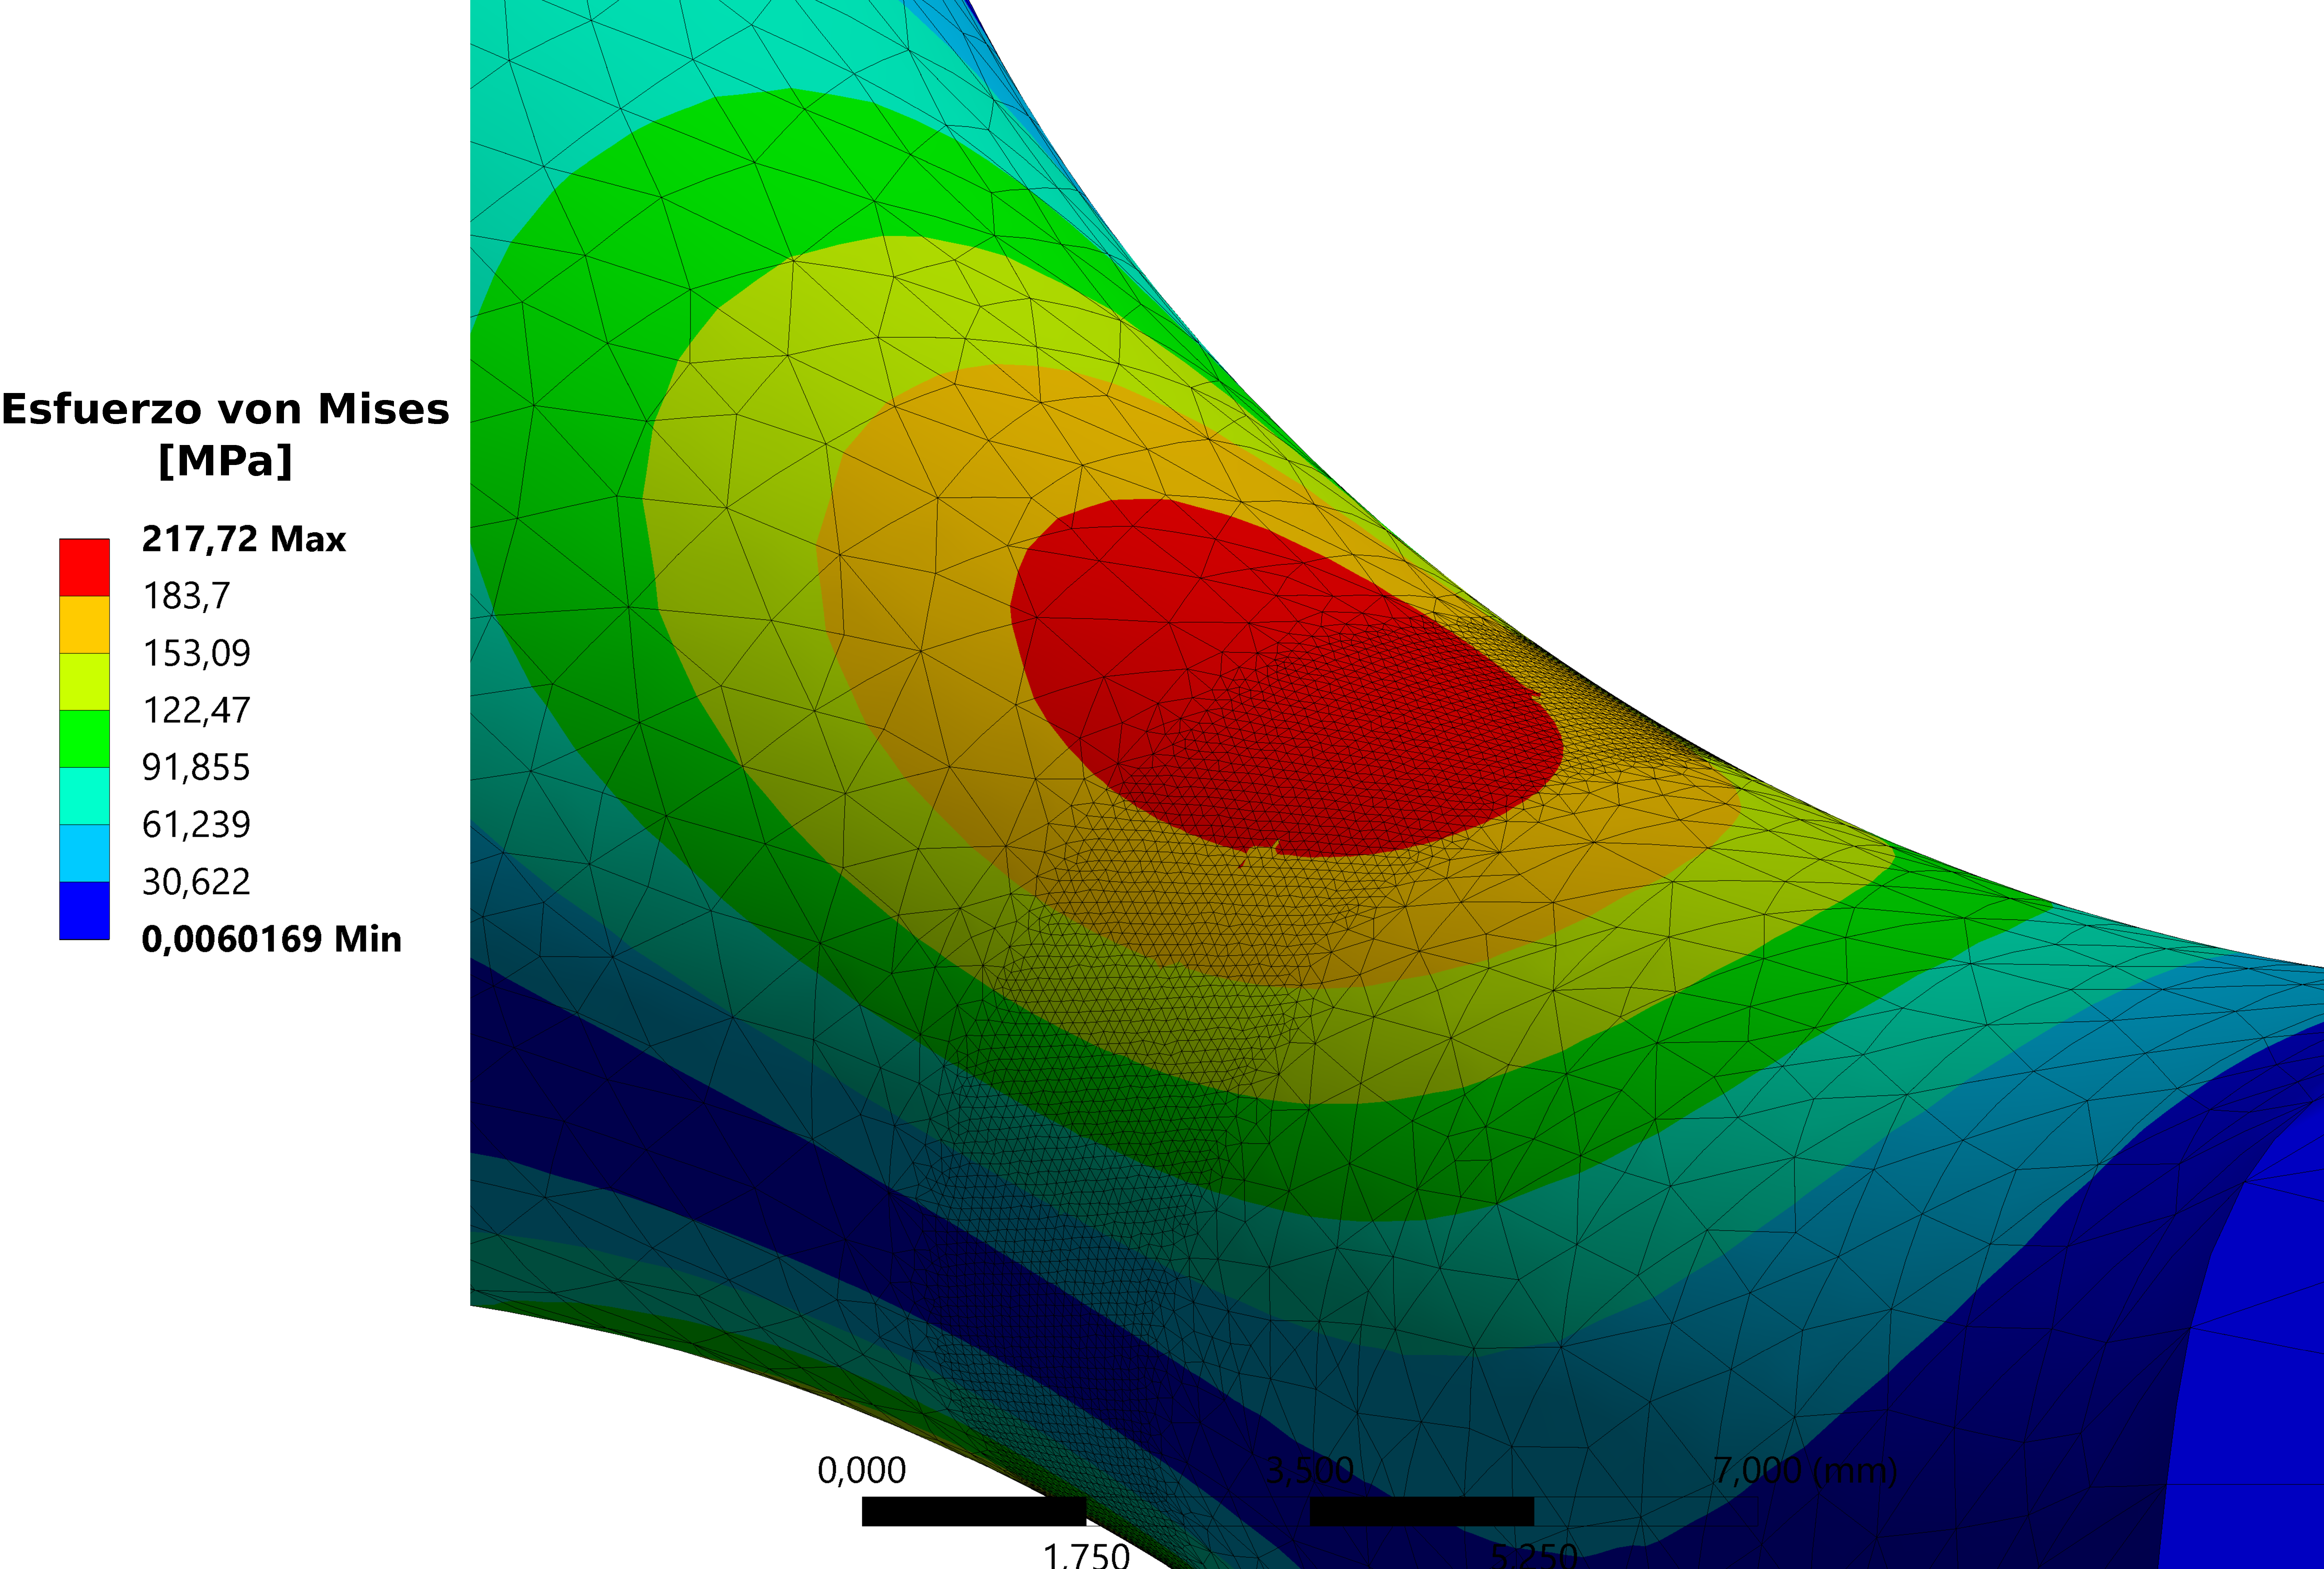
\includegraphics[width=\linewidth]{Imagenes/esfvm_iso.pdf}
		\caption{Vista en isométrico de la zona intermedia.}
		\label{fig:iso201}
	\end{subfigure}
\end{figure}
\begin{figure}[]
	\ContinuedFloat
	\centering
	\begin{subfigure}{0.9\linewidth}
		\centering
		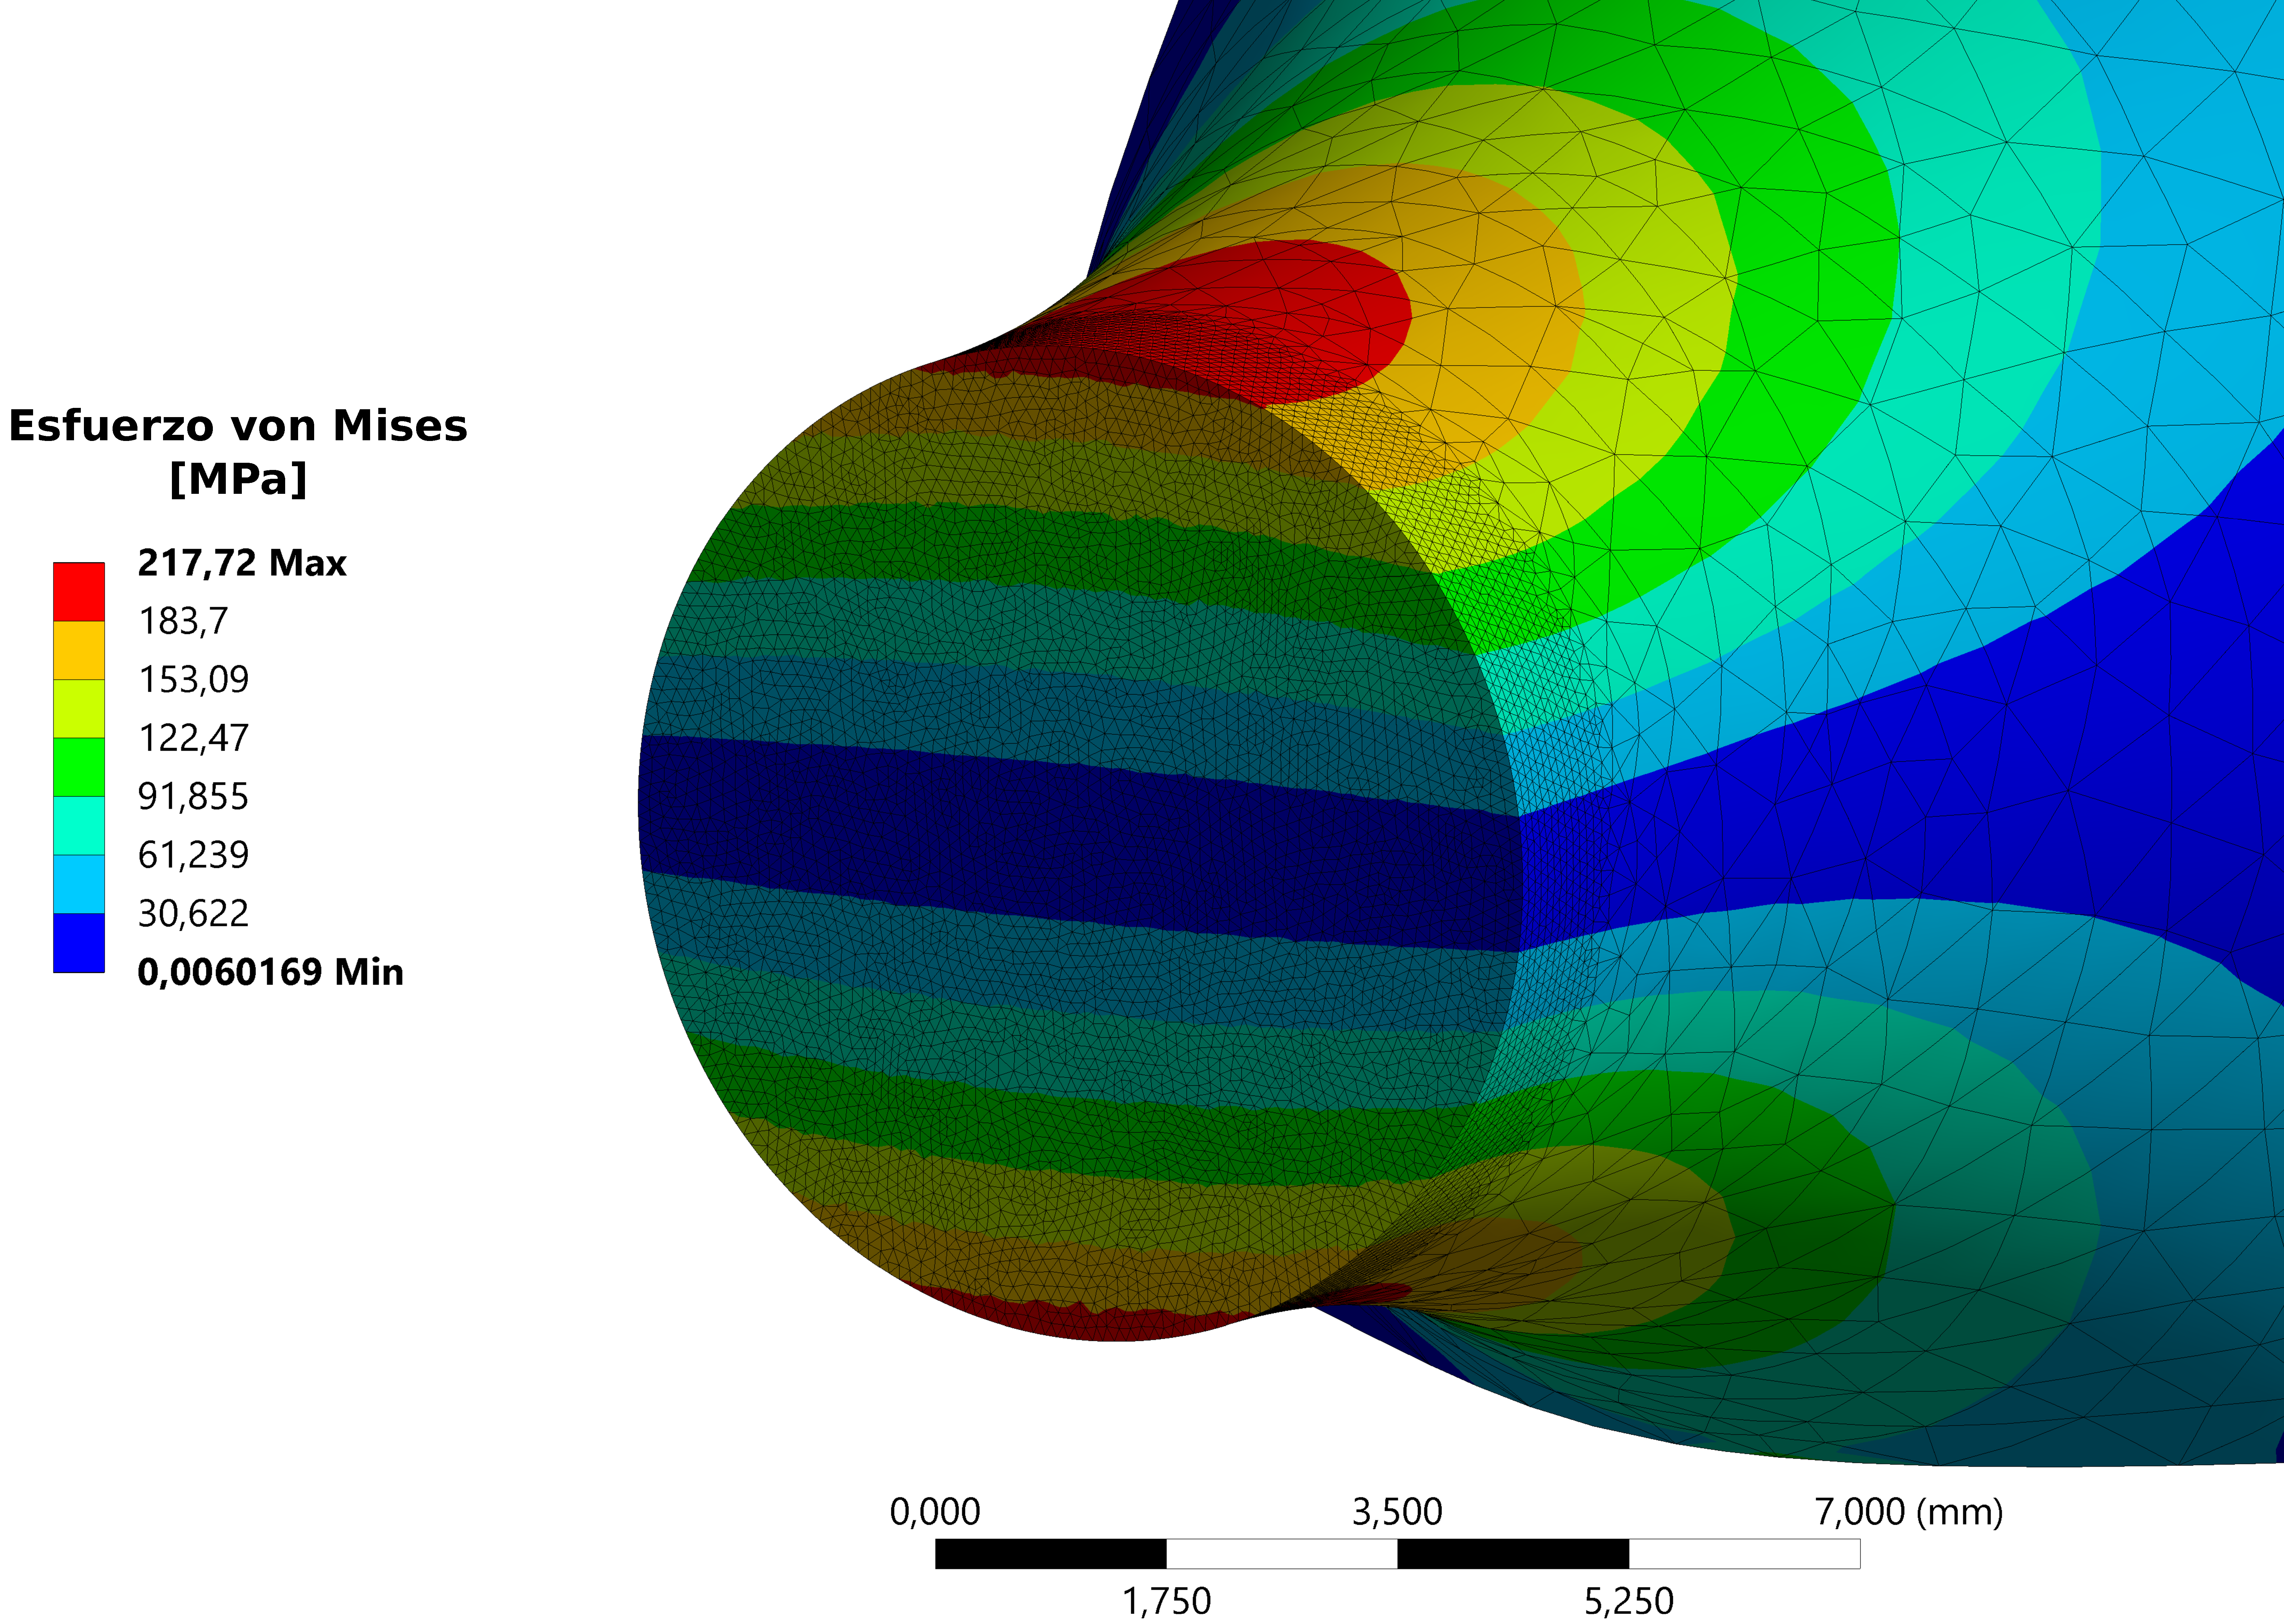
\includegraphics[width=\linewidth]{Imagenes/esfvm_corteiso.pdf}
		\caption{Vista en isométrico del corte transversal.}
		\label{fig:corte_iso201}
	\end{subfigure}		
	\begin{subfigure}{0.9\linewidth}
		\centering
		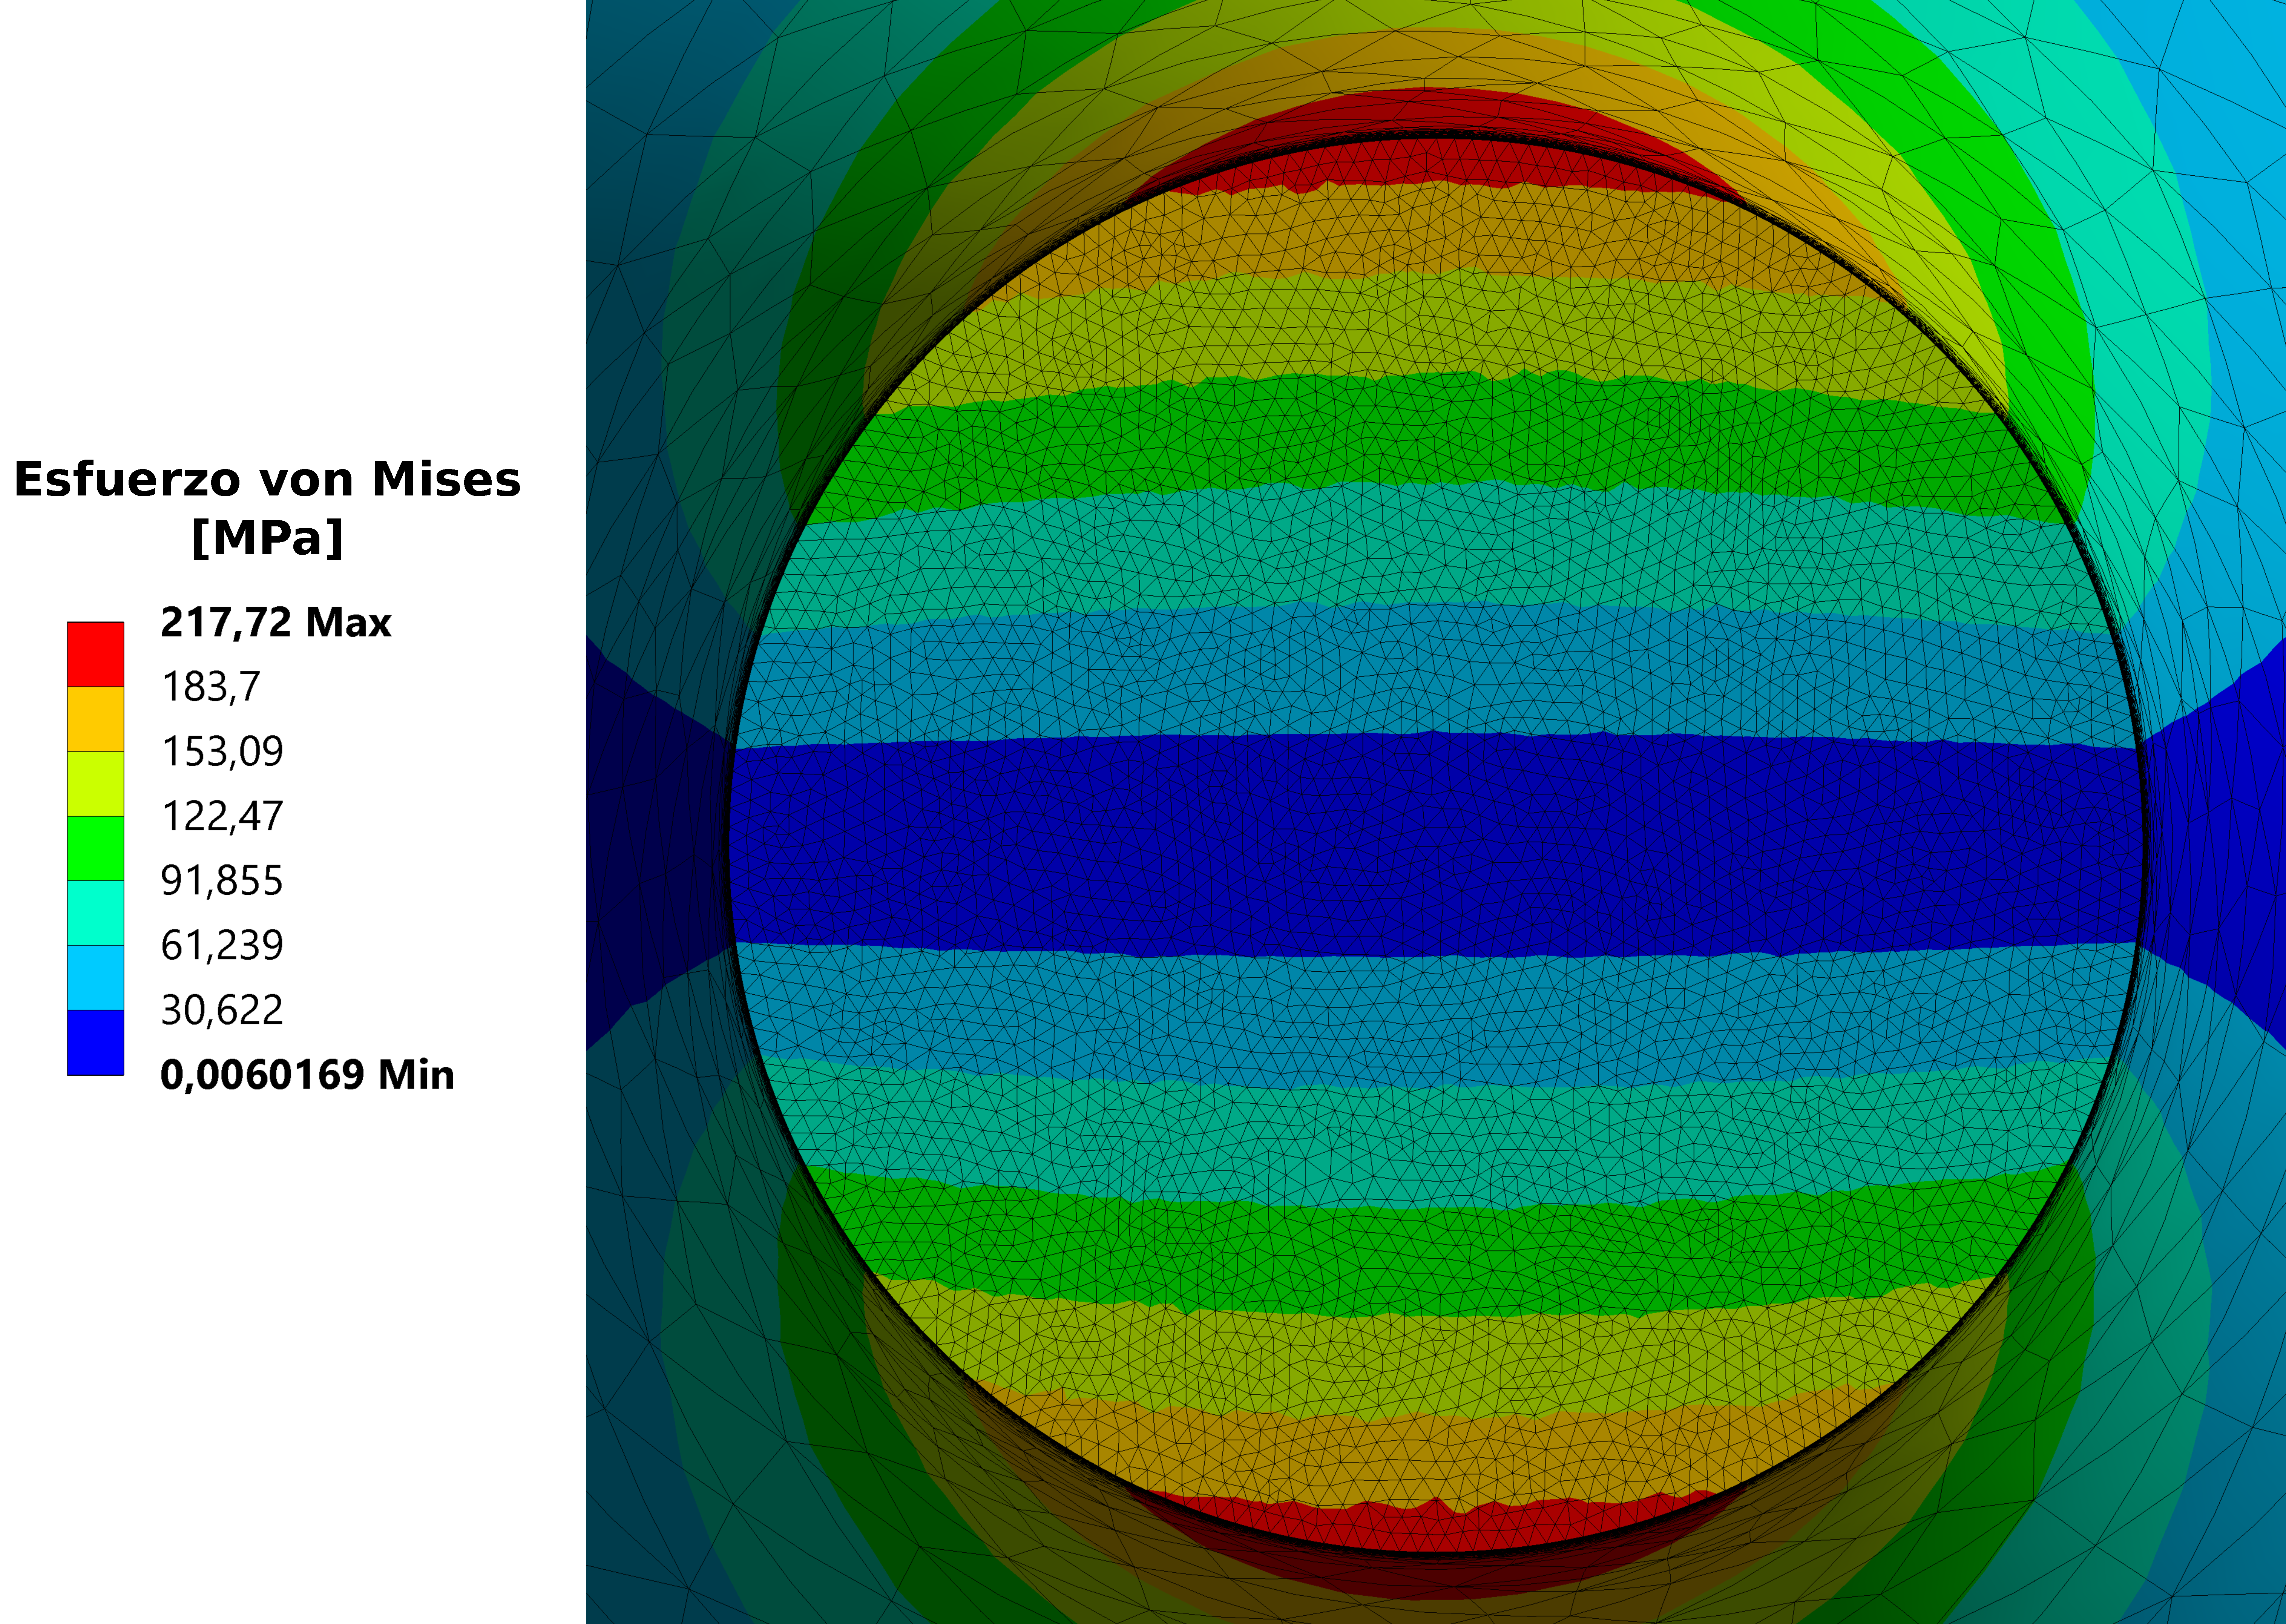
\includegraphics[width=\linewidth]{Imagenes/esfvm_corte.pdf}
		\caption{Vista en detalle del corte transversal.}
		\label{fig:corte201}
	\end{subfigure}
\caption{Detalle de la distribución de esfuerzos de von Mises en la zona intermedia de la probeta.}
\label{fig:resultados_vm}
\end{figure}

\newpage

Finalmente, como se buscan conocer los esfuerzos y la deformación a los que está sometida la probeta en estos puntos en específico, se obtienen los resultados de la deformación unitaria normal, cortante ($\varepsilon_x$) y de von Mises elástica ($\varepsilon_{vm,e}$), además de los esfuerzos de von Mises ($\sigma_{vm}$), cortante absoluto ($\tau_{max}$), normal ($\sigma_x$) y cortante ($\tau_{xy}$). Estos resultados se pueden ver en los gráficos \ref{fig:def_201} y \ref{fig:esf_201}.

\begin{figure}[h]
\centering
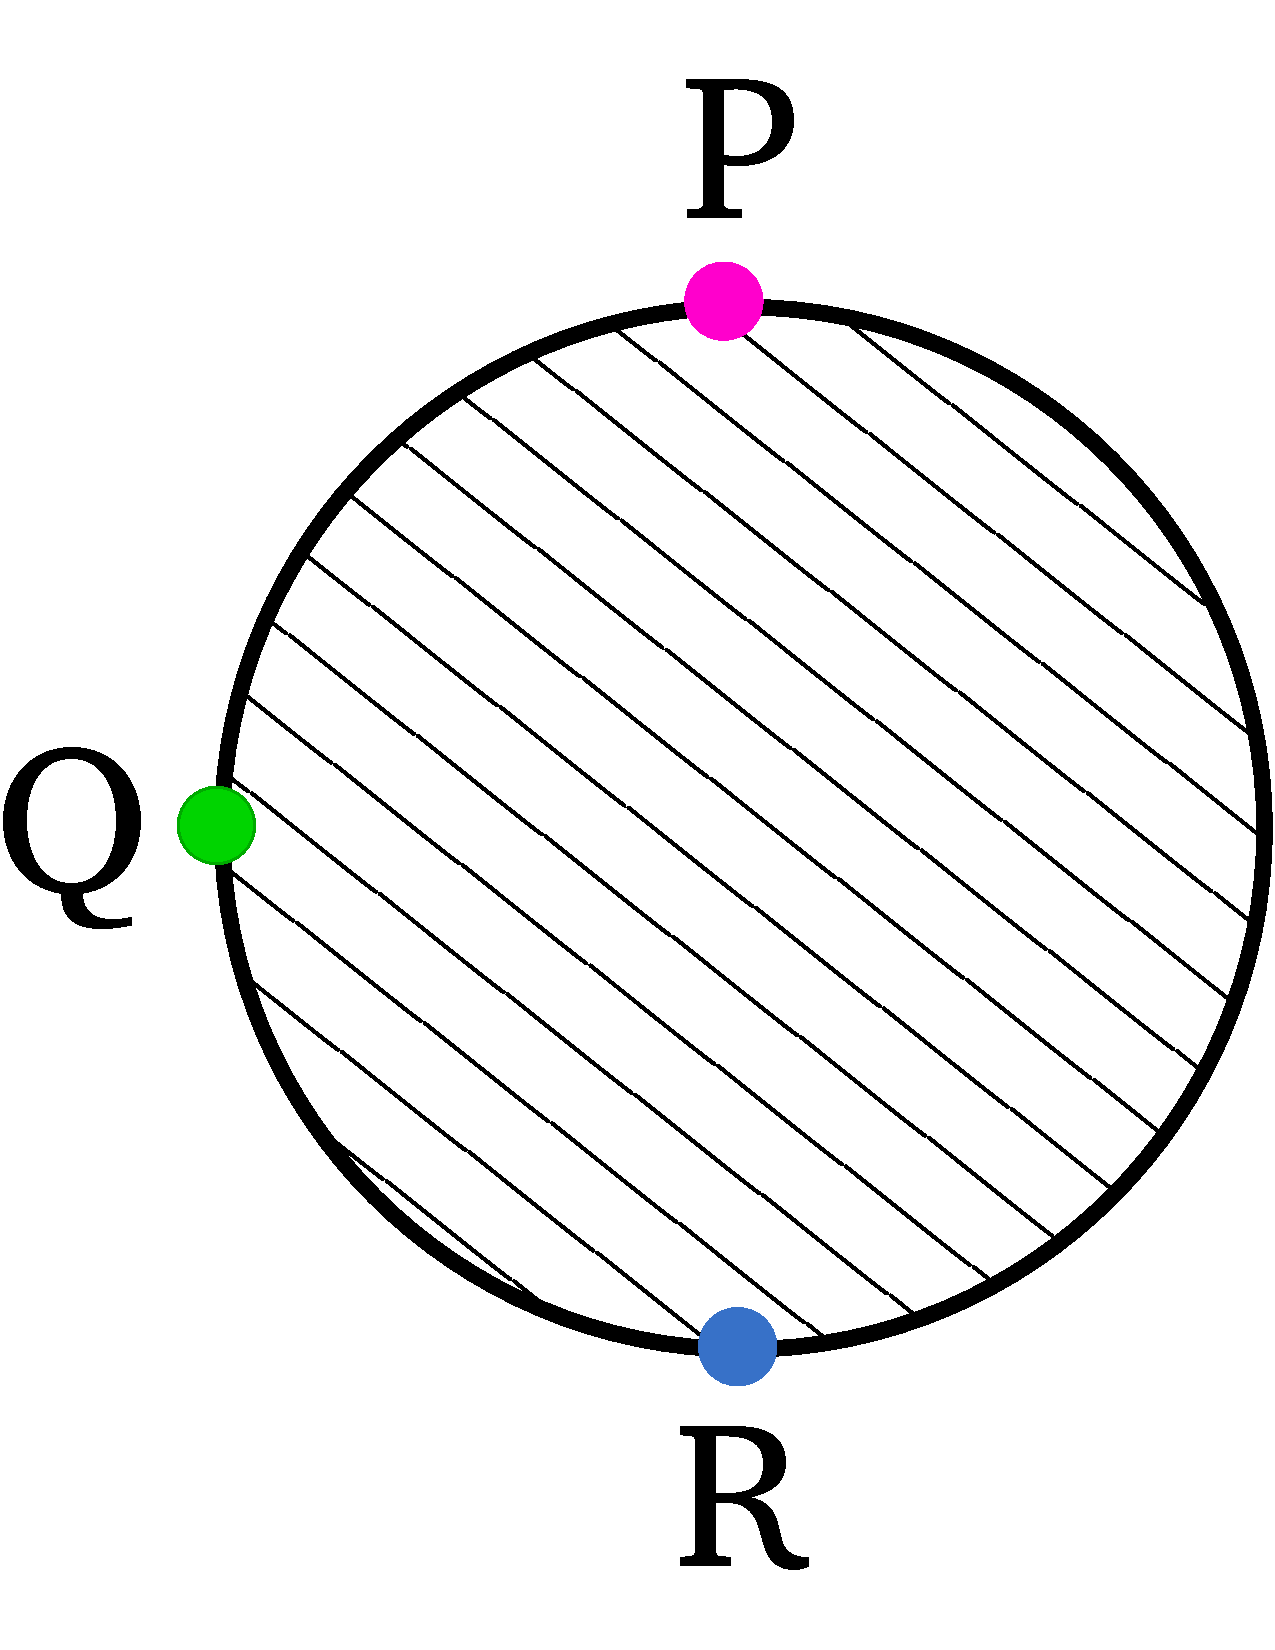
\includegraphics[width=0.2\linewidth]{Imagenes/diagelem_pqr.pdf}
\caption{Ubicación de los elementos $P$, $Q$ y $R$}
\label{fig:diag_pqr2}
\end{figure}

Al ver el comportamiento lineal de los gráficos, se concluye que en ninguna configuración se superó el esfuerzo de fluencia, como también lo confirman los datos de esfuerzo obtenidos. Los resultados del esfuerzo de von Mises ($\sigma_{vm}$), absoluto ($\tau_{abs}$) y normal ($\sigma_x$) máximo se encuentran en los punto $P$ y $R$, siendo el segundo levemente mayor por $0.1$ MPa en promedio. En el caso del esfuerzo cortante ($\tau_{xy}$) máximo se encuentra en el punto $Q$, como es esperable al estar cerca del eje neutro. Los resultados de la carga, deformación y esfuerzos se muestran en la tabla \ref{tab:res_esf} para las combinaciones n$^{\circ}$ 1, 100 y 201, además de la carga media ($F_m$). En la tabla \ref{sec:anexob2} se encuentran los resultados completos para cada combinación de los esfuerzos de von Mises y absoluto.

\begin{table}[h]
\centering
\resizebox{\textwidth}{!}{%
\begin{tabular}{@{}ccccccc@{}}
\toprule
Resultados    & \multicolumn{1}{c}{Fuerza {[}N{]}} & \begin{tabular}[c]{@{}c@{}}Deformación eje $y$\\  {[}mm{]}\end{tabular} & $\sigma_{vm}$ {[}MPa{]} & $\tau_{abs}$ {[}MPa{]} & $\sigma_{x}$ {[}MPa{]} & $\tau_{xy}$ {[}MPa{]} \\ \midrule
$F_{max,1}$   & $13.71$                            & $-0.0078$                                                               & $9.376$                 & $4.7752$               & $-9.606$               & $0.38138$             \\
$F_{max,100}$ & $131.14$                           & $-0.0743$                                                               & $88.529$                & $45.312$               & $-91.151$              & $3.5809$              \\
$F_{max,201}$ & $296.914$                          & $-0.16969$                                                              & $203.13$                & $103.46$               & $-208.12$              & $8.2478$              \\
$F_m$         & $12.438$                           & $-0.0071$                                                               & $9.124$                 & $4.6315$               & $-9.4519$              & $1.9199$              \\ \bottomrule
\end{tabular}%
}
\caption{Carga, deformación y esfuerzos obtenidos por medio de la simulación para la combinación n$^{\circ}$ 1, 100 y 201, además de los esfuerzos provocados por la carga media.}
\label{tab:res_esf}
\end{table}

\newpage

\begin{figure}[H]
\centering
	\begin{subfigure}{1\linewidth}
		\centering
		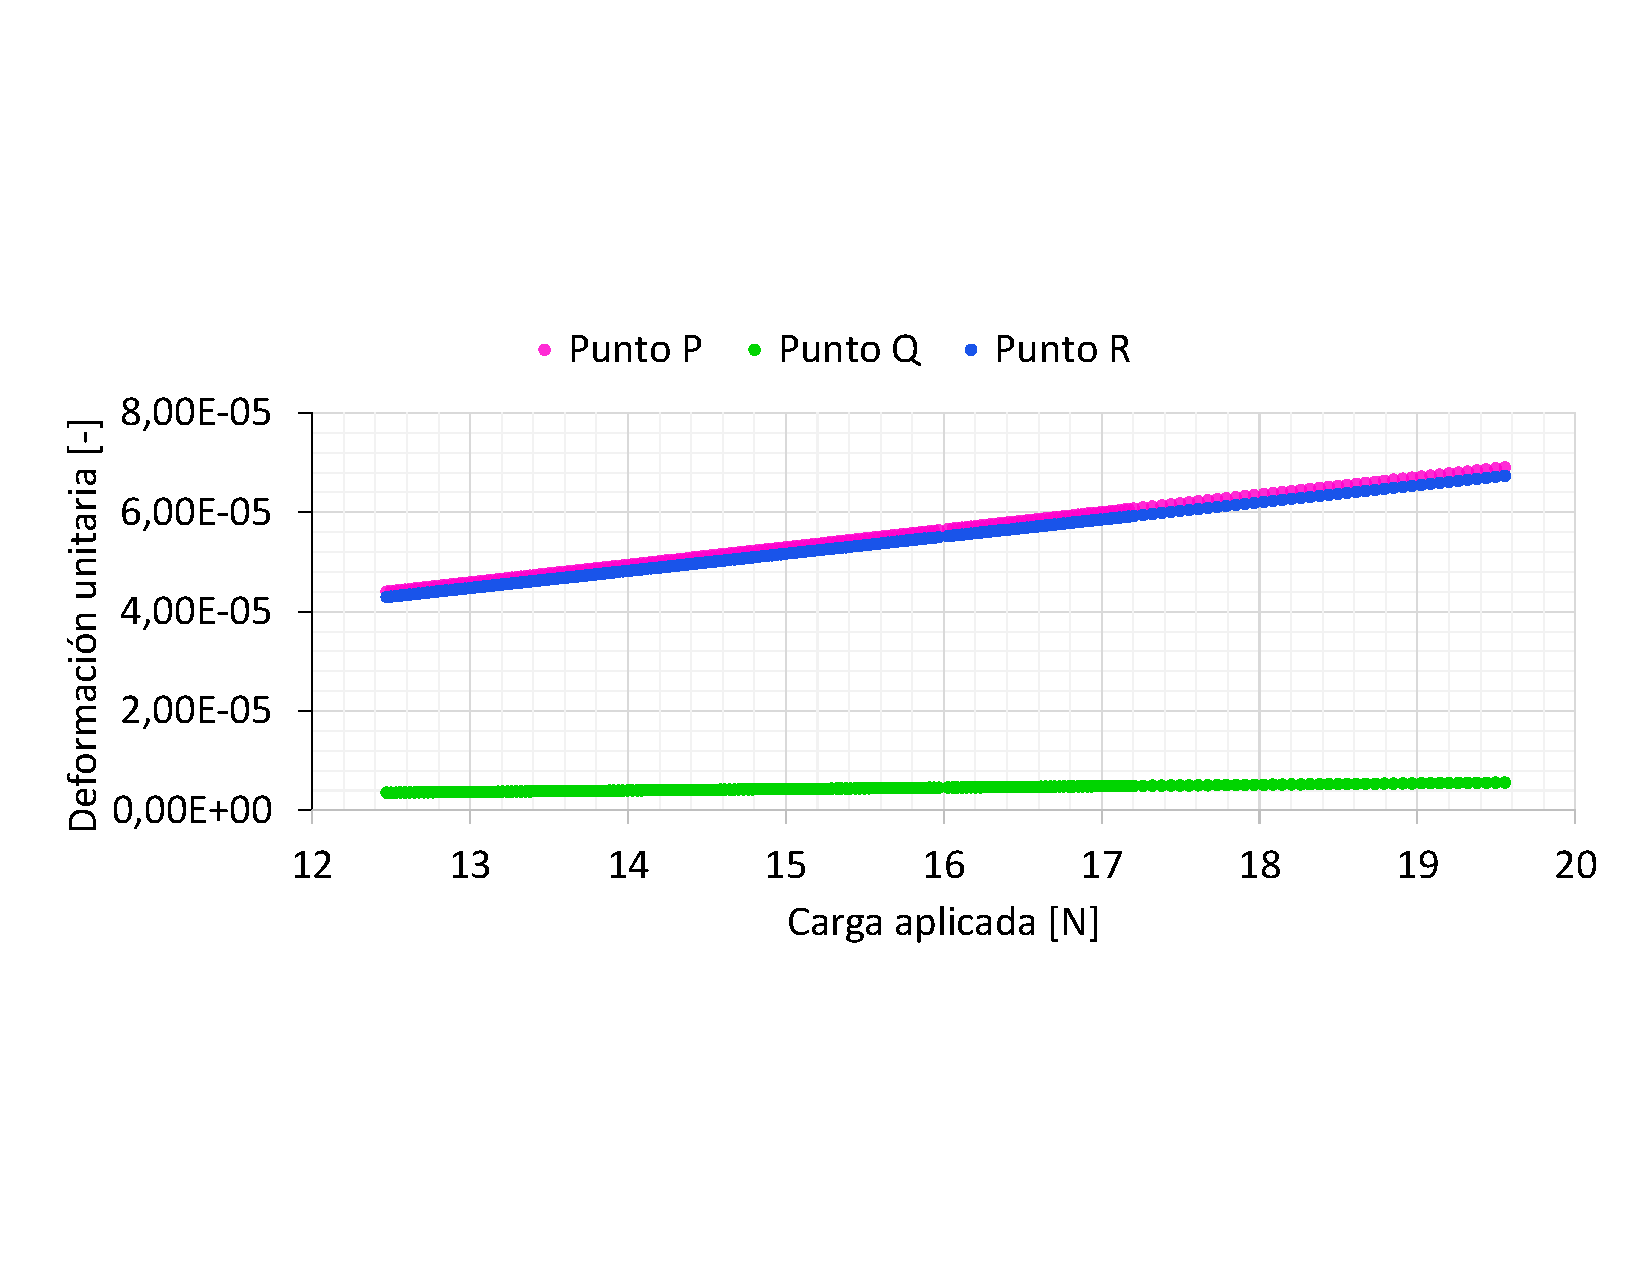
\includegraphics[width=\linewidth, trim={1cm 0cm 2cm 0cm},clip]{Imagenes/def_vm.pdf}
		\caption{Deformación de von Mises de los puntos $P$, $Q$ y $R$.}
		\label{fig:def_normal201}
	\end{subfigure}
		\begin{subfigure}{1\linewidth}
		\centering
		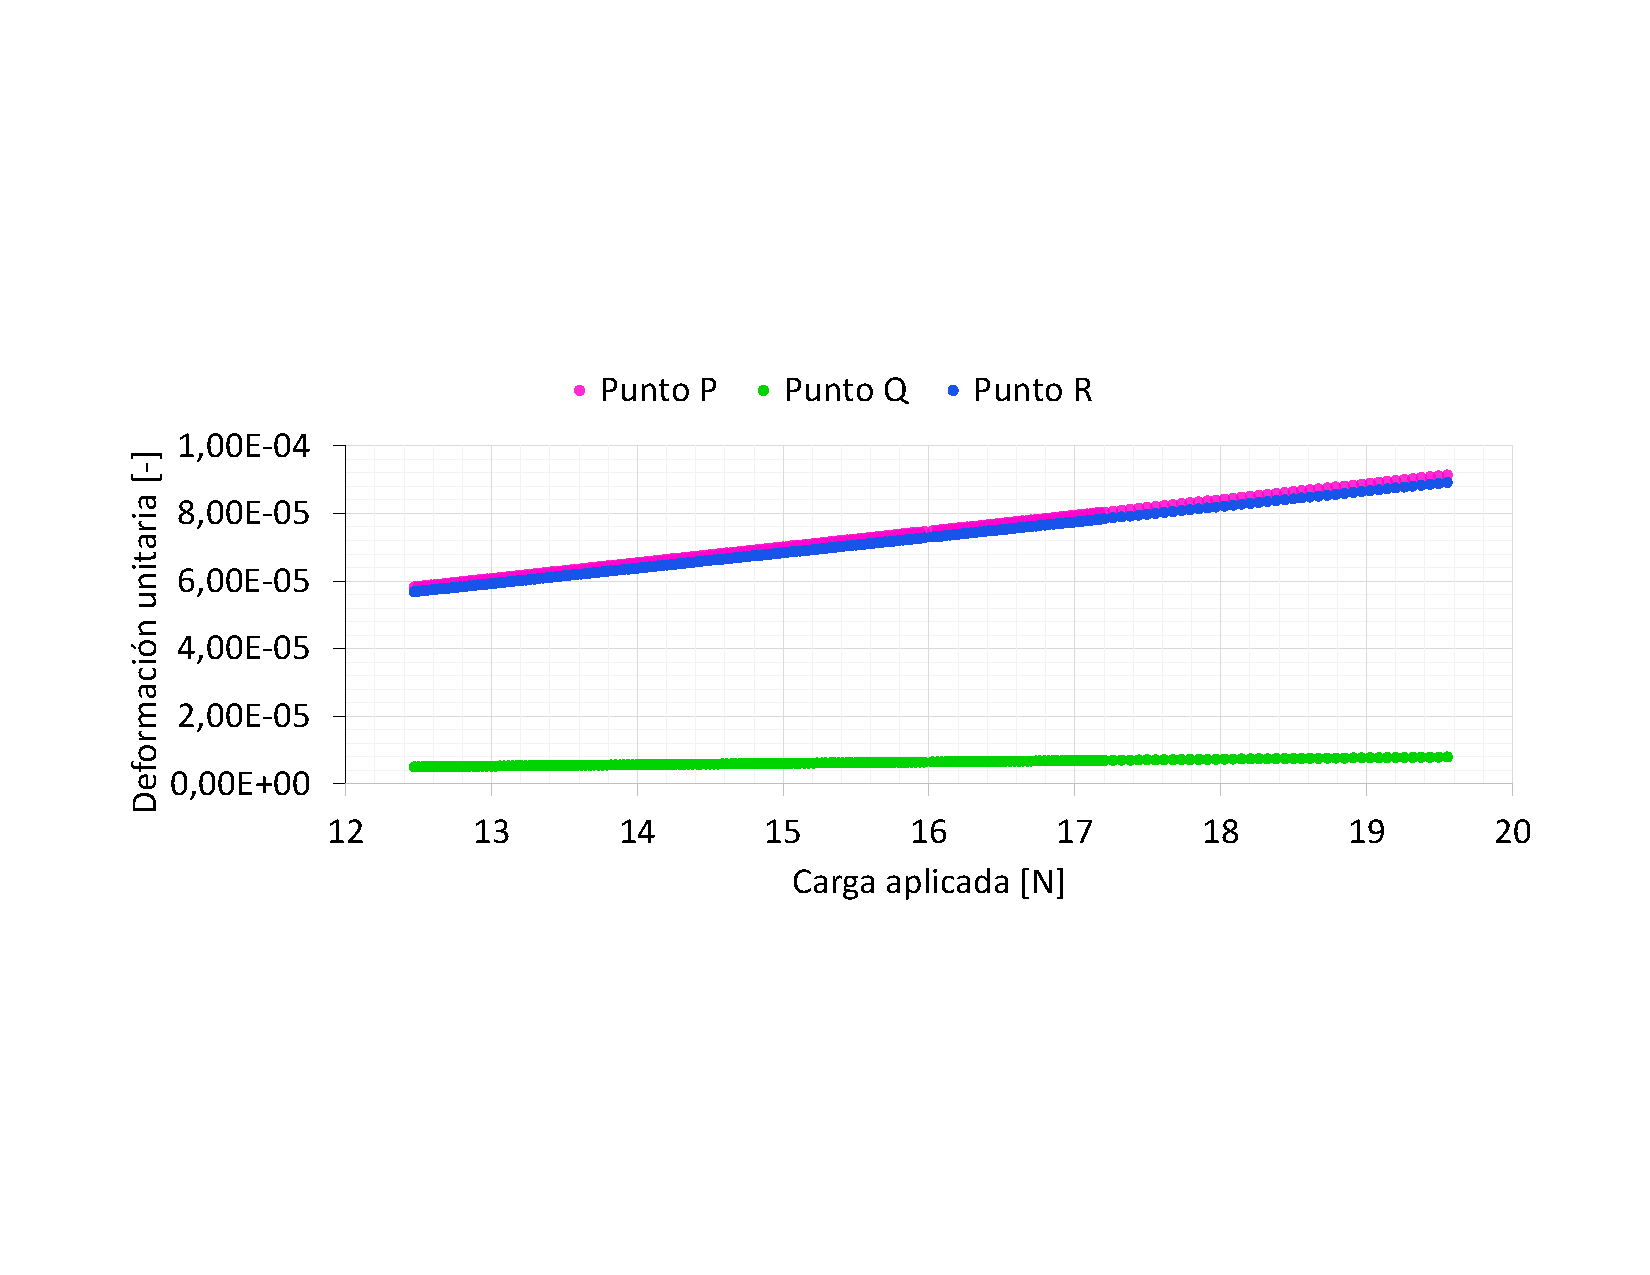
\includegraphics[width=\linewidth, trim={1cm 0cm 2cm 0cm},clip]{Imagenes/def_ms.pdf}
		\caption{Deformación cortante absoluta de los puntos $P$, $Q$ y $R$.}
		\label{fig:def_vm201}
	\end{subfigure}
\end{figure}

\begin{figure}[p]
\centering
\ContinuedFloat
	\begin{subfigure}{1\linewidth}
		\centering
		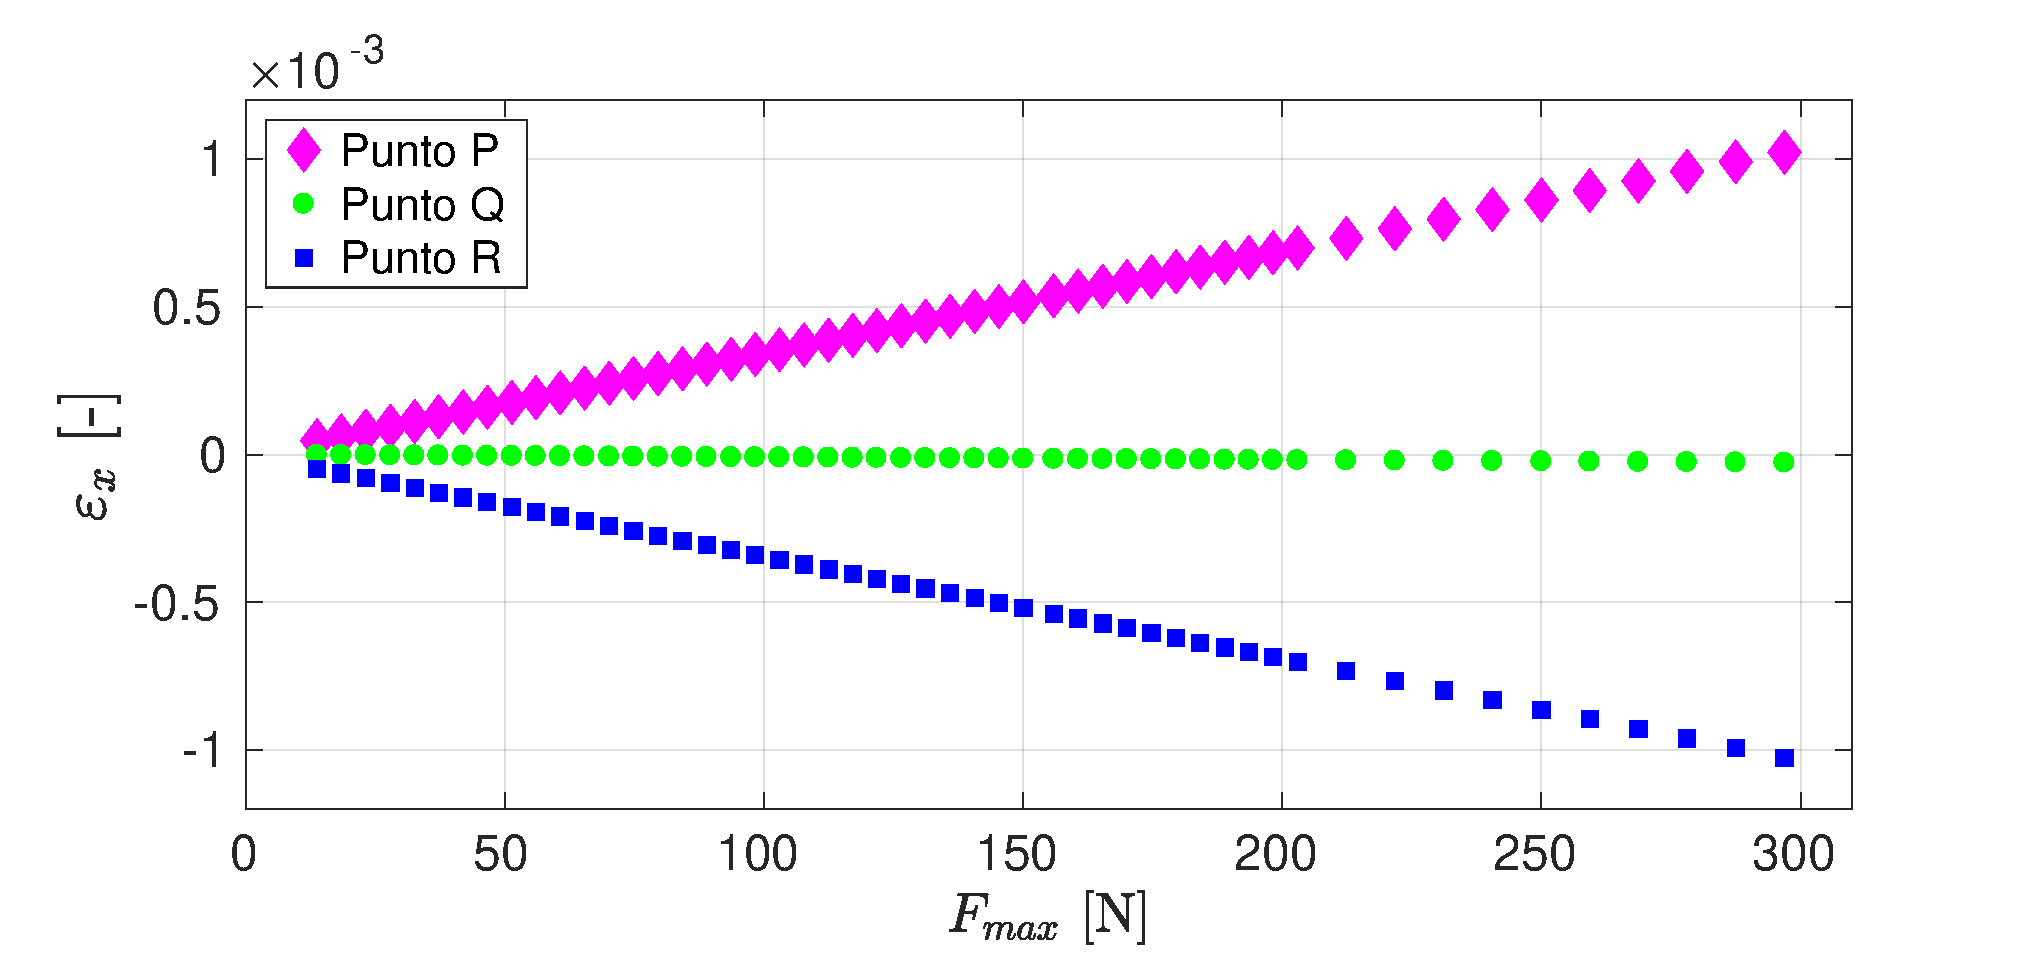
\includegraphics[width=\linewidth, trim={1cm 0cm 2cm 0cm},clip]{Imagenes/def_normal.pdf}
		\caption{Deformación normal, en dirección $x$, de los puntos $P$, $Q$ y $R$.}
		\label{fig:def_normal201}
	\end{subfigure}
		\begin{subfigure}{1\linewidth}
		\centering
		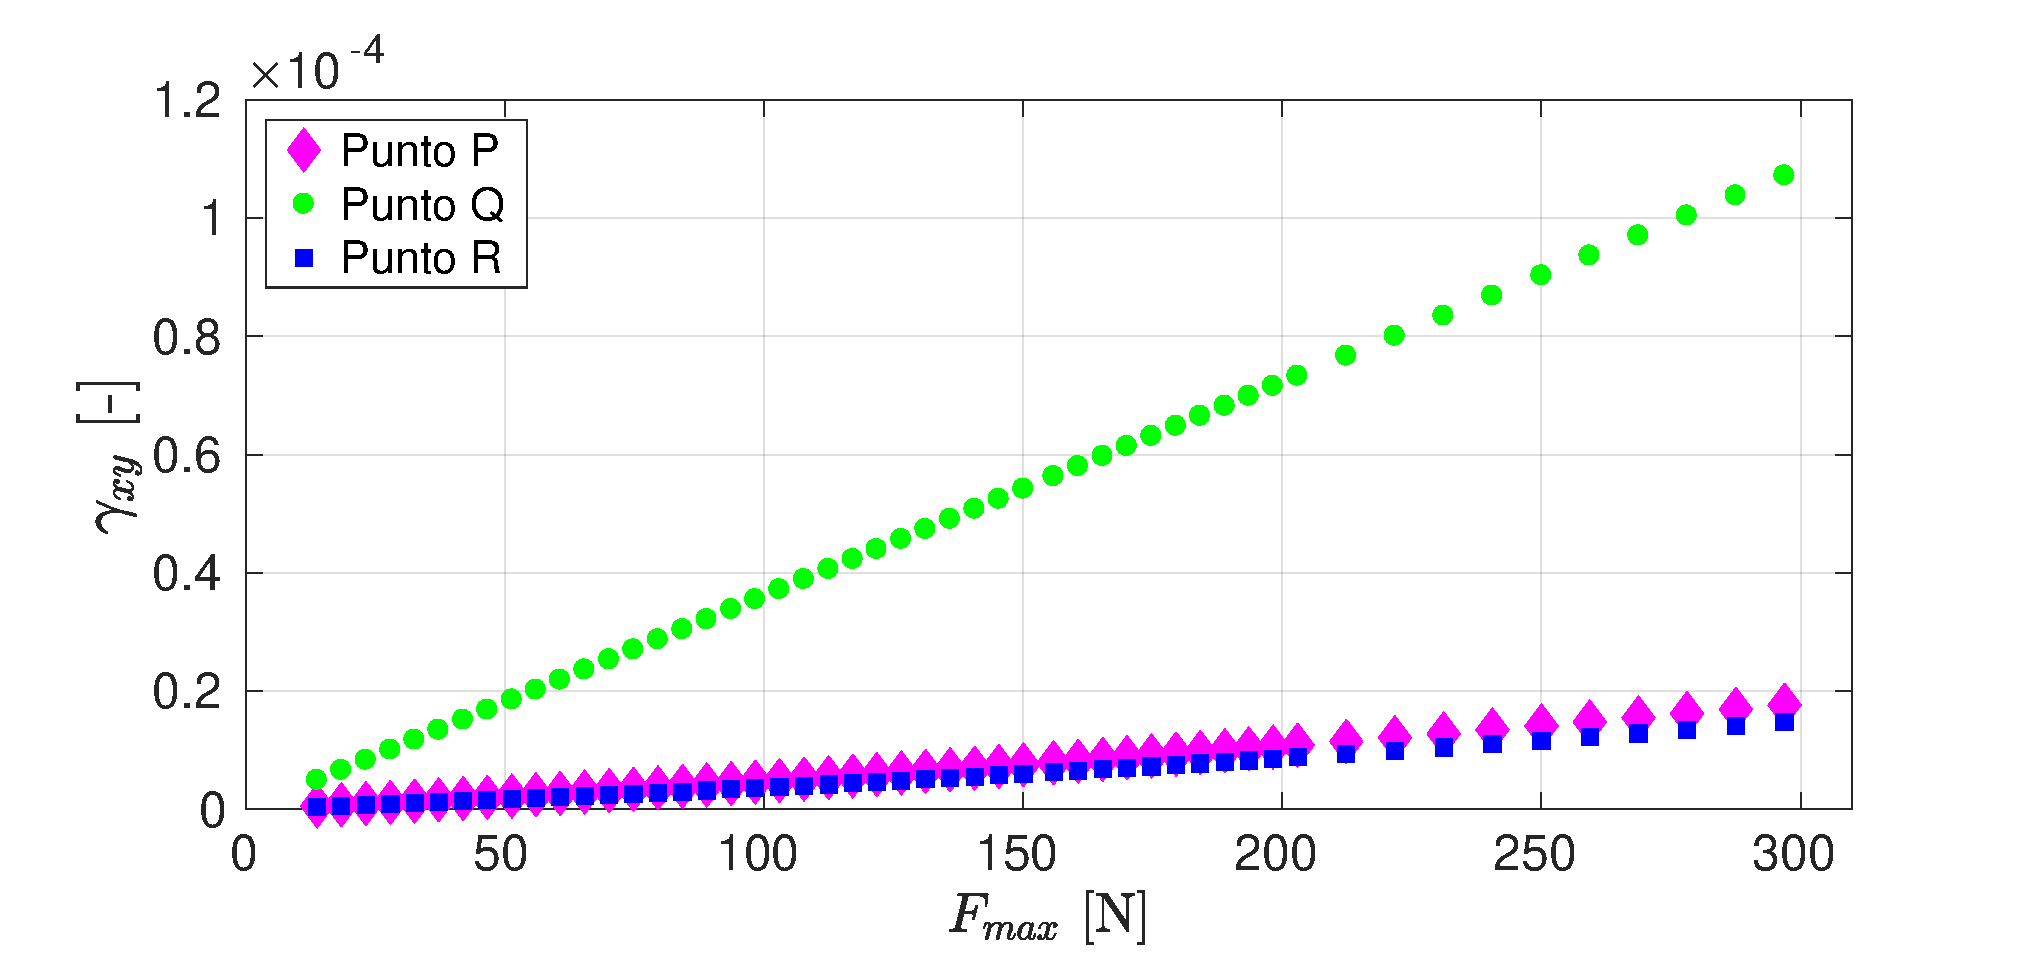
\includegraphics[width=\linewidth, trim={1cm 0cm 2cm 0cm},clip]{Imagenes/def_cortante.pdf}
		\caption{Deformación cortante, en dirección $y$ del plano \textit{YZ}, de los puntos $P$, $Q$ y $R$.}
		\label{fig:def_vm201}
	\end{subfigure}
\caption{Deformación unitaria de los puntos $P$, $Q$ y $R$  }
\label{fig:def_201}
\end{figure}

\begin{figure}[H]
\centering
	\begin{subfigure}{1\linewidth}
		\centering
		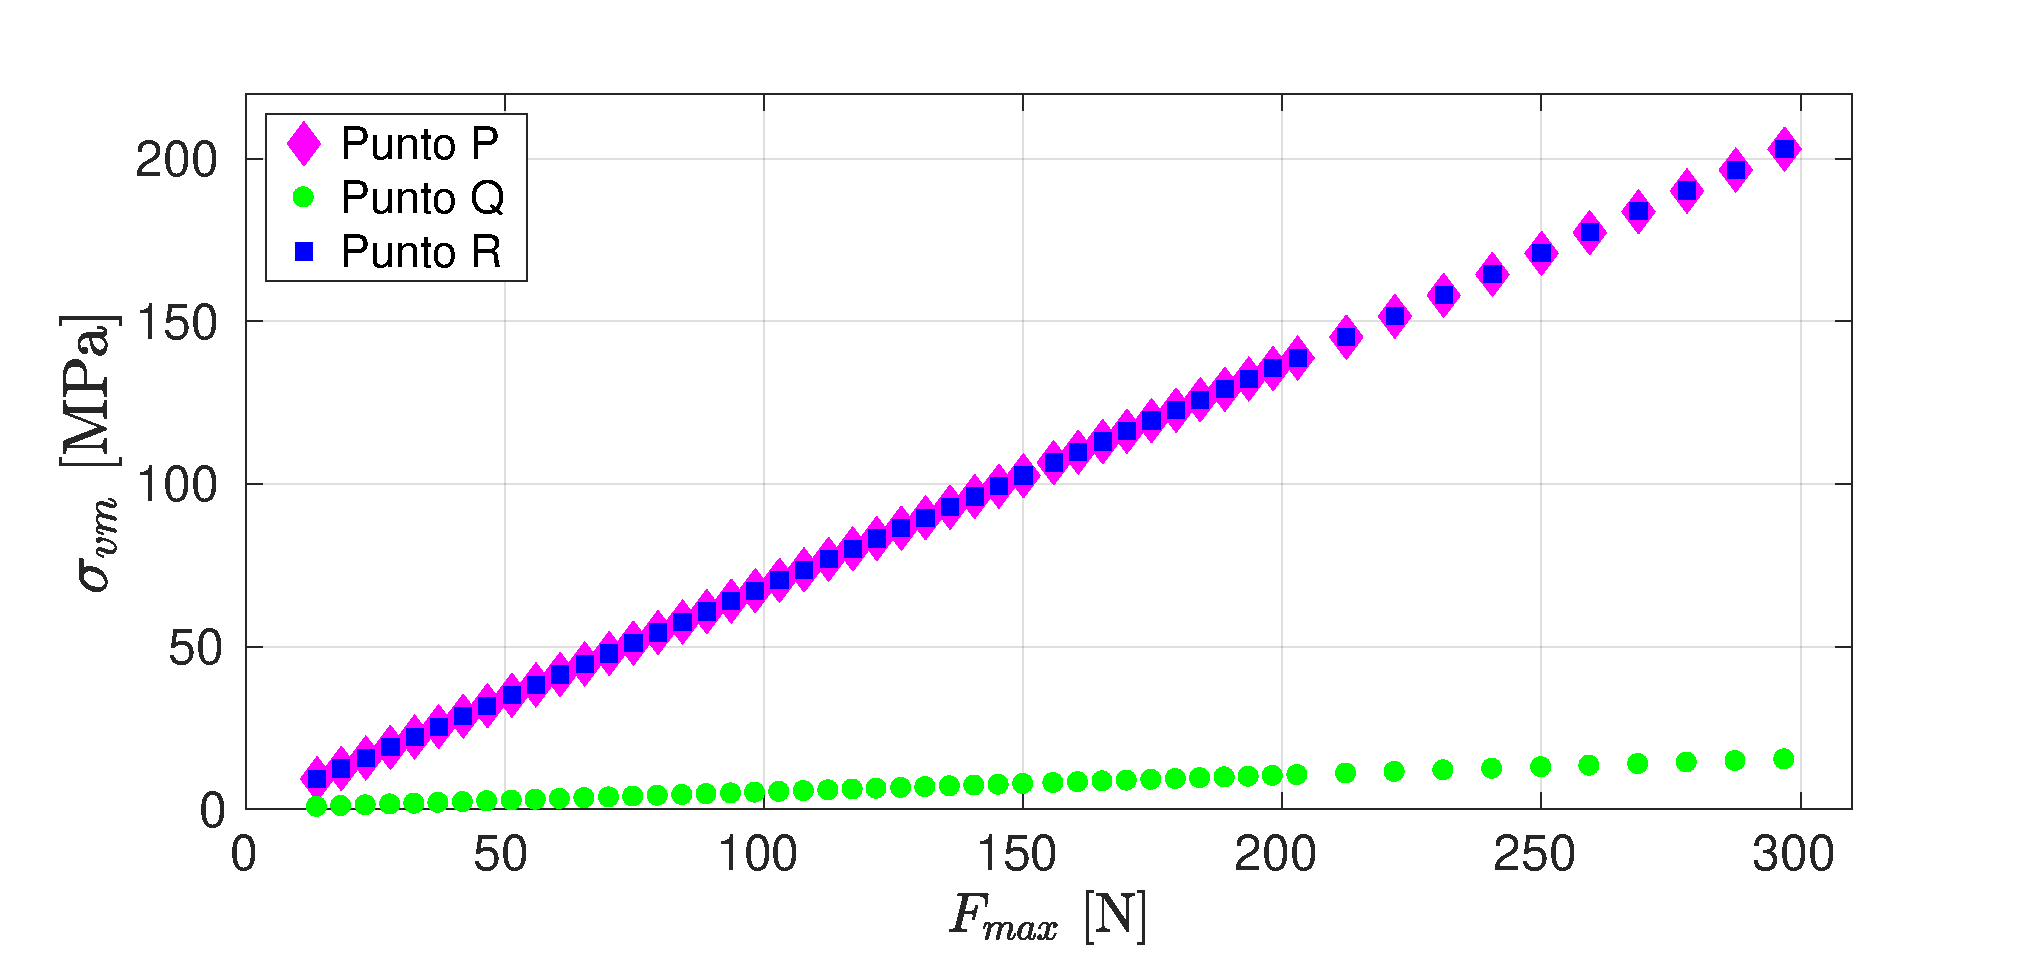
\includegraphics[width=\linewidth, trim={1cm 0cm 2cm 0cm},clip]{Imagenes/esf_vm.pdf}
		\caption{Esfuerzo de von Mises de los puntos $P$, $Q$ y $R$.}
		\label{fig:esf_vm201}
	\end{subfigure}
	\begin{subfigure}{1\linewidth}
		\centering
		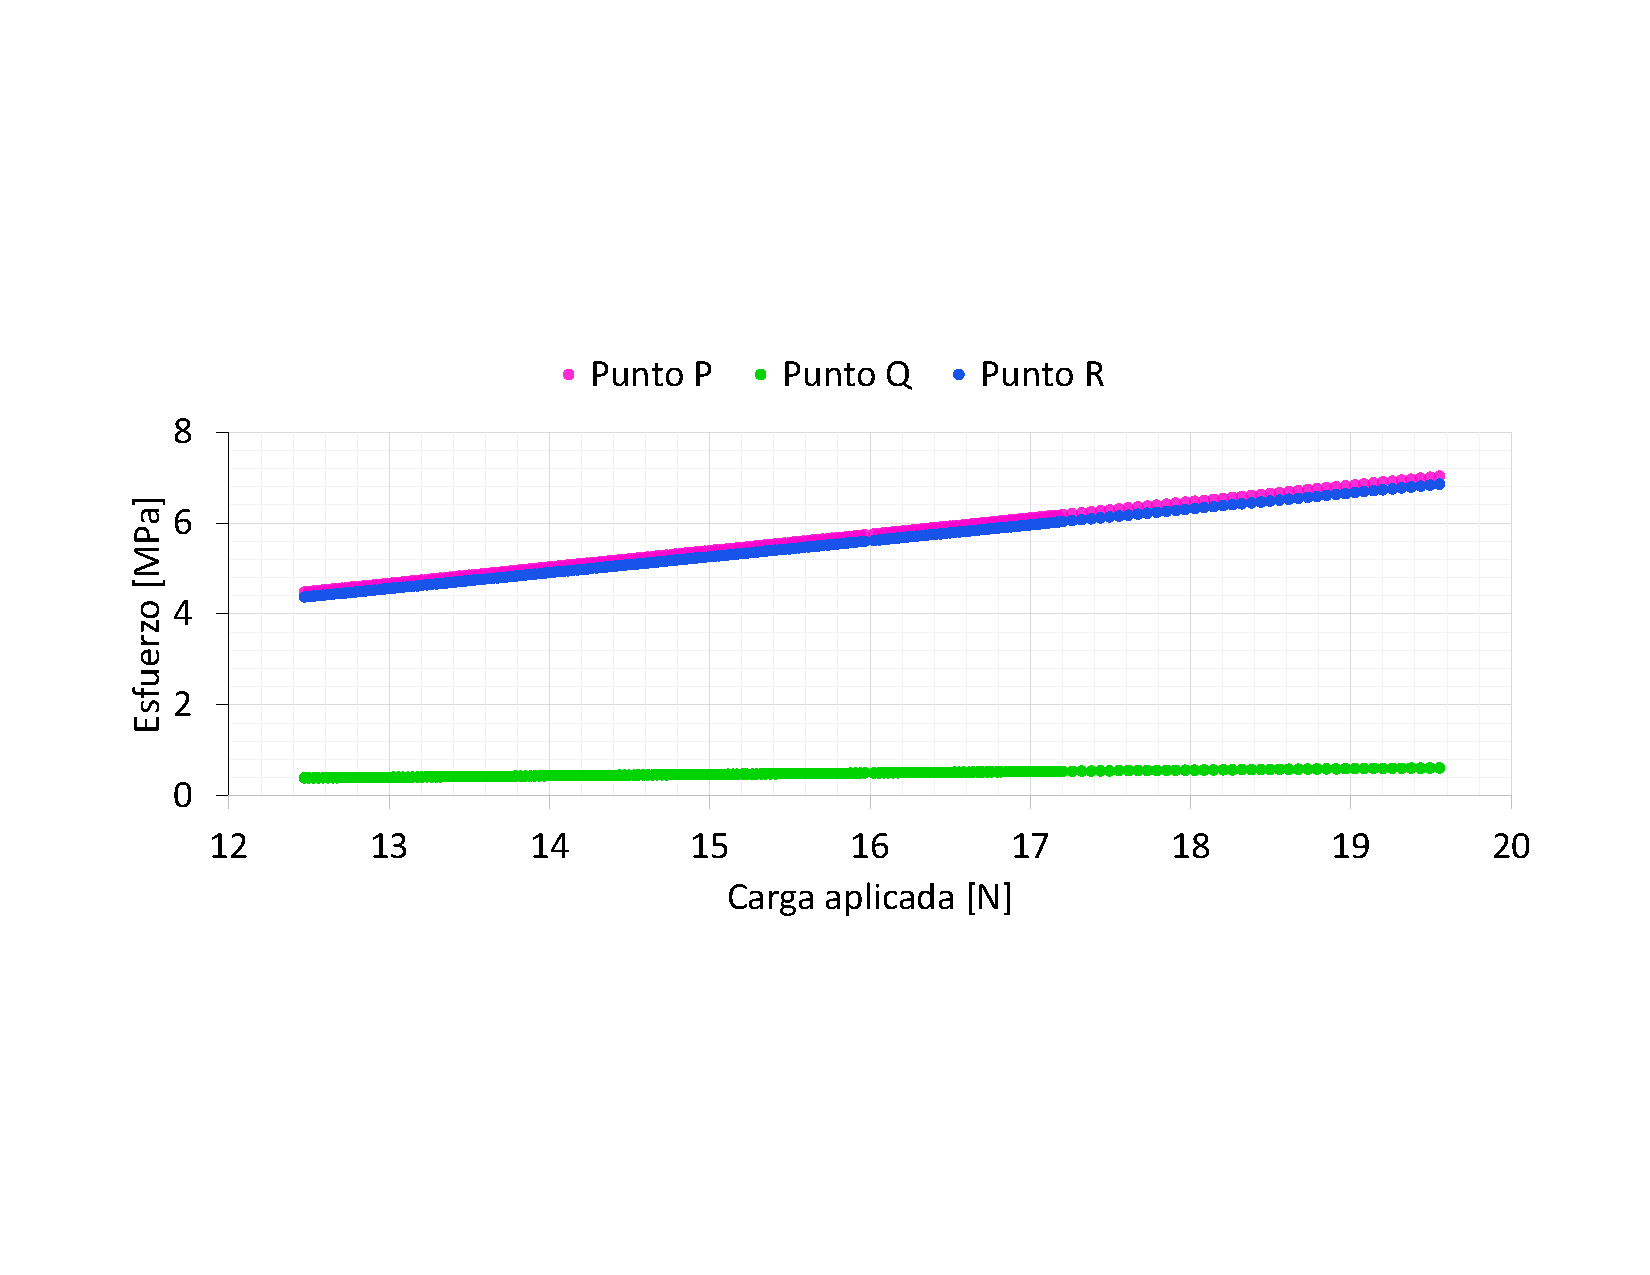
\includegraphics[width=\linewidth, trim={1cm 0cm 2cm 0cm},clip]{Imagenes/esf_ms.pdf}
		\caption{Esfuerzo cortante absoluto de los puntos $P$, $Q$ y $R$.}
		\label{fig:esf_ms201}
	\end{subfigure}
\end{figure}

\begin{figure}[p]
\centering
	\ContinuedFloat
	\begin{subfigure}{1\linewidth}
		\centering
		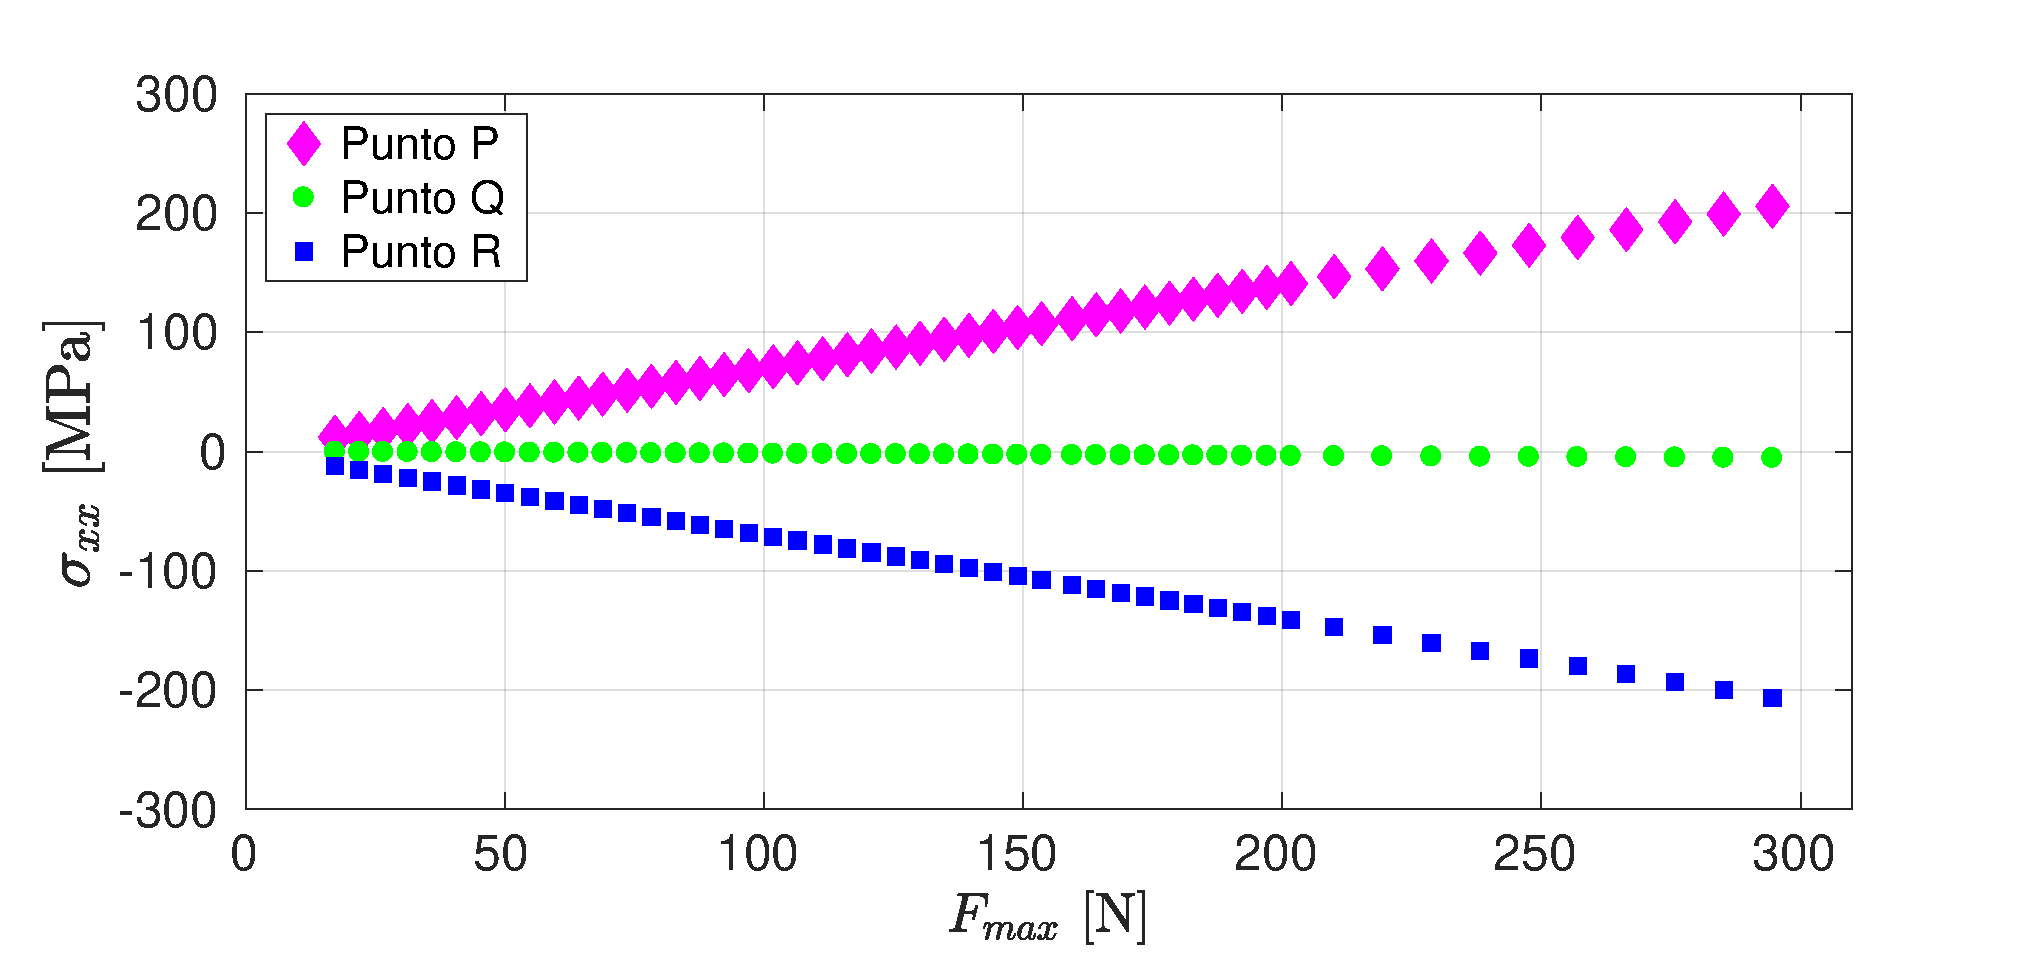
\includegraphics[width=\linewidth, trim={0cm 0cm 2cm 0cm},clip]{Imagenes/esf_normal.pdf}
		\caption{Esfuerzo normal, en dirección $x$, de los puntos $P$, $Q$ y $R$.}
		\label{fig:esf_normal201}
	\end{subfigure}
	\begin{subfigure}{1\linewidth}
		\centering
		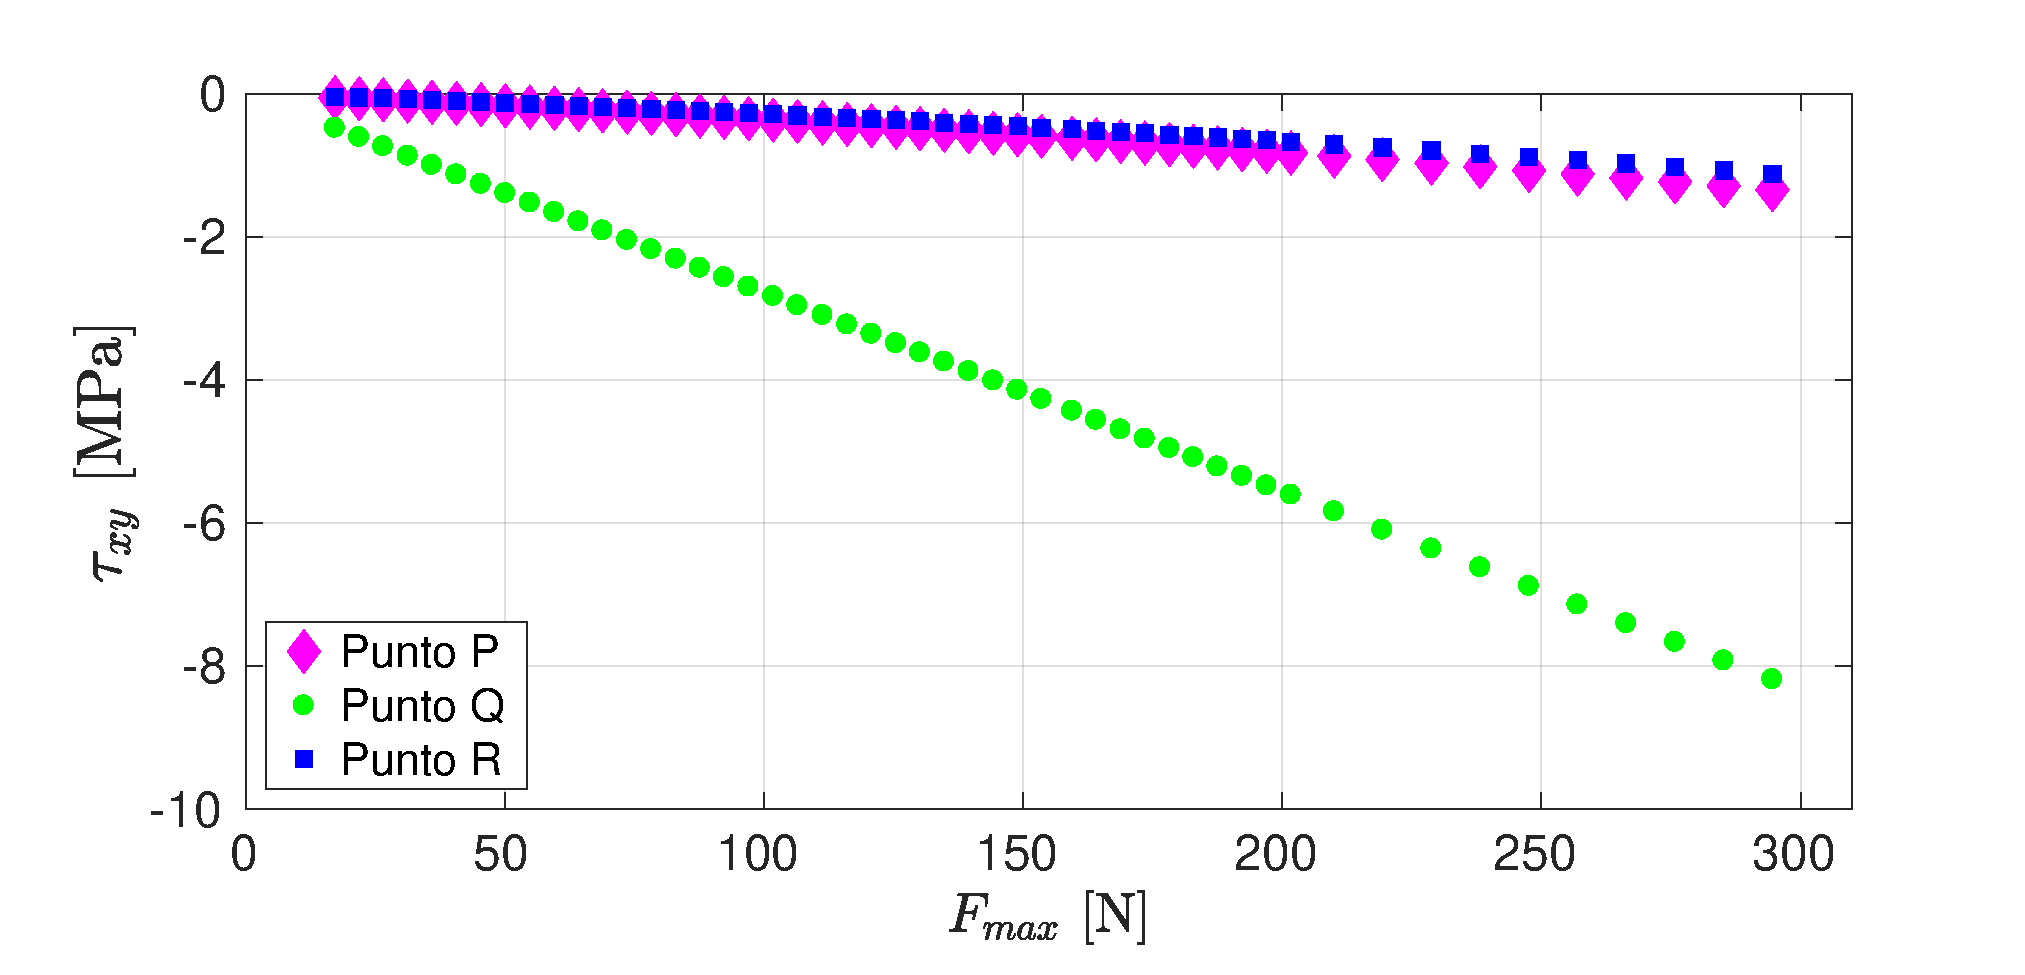
\includegraphics[width=\linewidth, trim={1cm 0cm 2cm 0cm},clip]{Imagenes/esf_cortante.pdf}
		\caption{Esfuerzo cortante, en dirección $y$ del plano \textit{YZ}, de los puntos $P$, $Q$ y $R$.}
		\label{fig:esf_ms201}
	\end{subfigure}
\caption{Esfuerzos de von Mises, cortante absoluto, normal y cortante de los puntos $P$, $Q$ y $R$.}
\label{fig:esf_201}
\end{figure}

\newpage

Al comparar los resultados obtenidos (anexo \ref{sec:anexob2}) con la tabla de cargas (anexo \ref{sec:anexob1}) se encuentran diferencias en los esfuerzos obtenidos para una misma configuración. Esta diferencia aumenta de manera constante a medida que aumenta la carga, por lo tanto, la relación de $\Delta m$ y $\sigma_{vm}$ es distinta entre el modelo y la información original, dicho de otra forma, la pendiente de sus curvas son distintas, como se ve en la fig. \ref{fig:comp_modtab}. Esto, sin duda, provoca dudas sobre la información que entregada por la tabla de cargas, sobre la veracidad y factibilidad de los esfuerzos que acompañan a cada combinación. Respecto a este último punto, resalta el hecho que en la tabla de cargas aparezcan esfuerzos que sean muy superiores a los que un acero pueda soportar. No obstante, se requiere de una validación experimental que determinará su precisión, tanto del desarrollo de esta tesis como de la tabla de carga.

\begin{figure}[h]
\centering
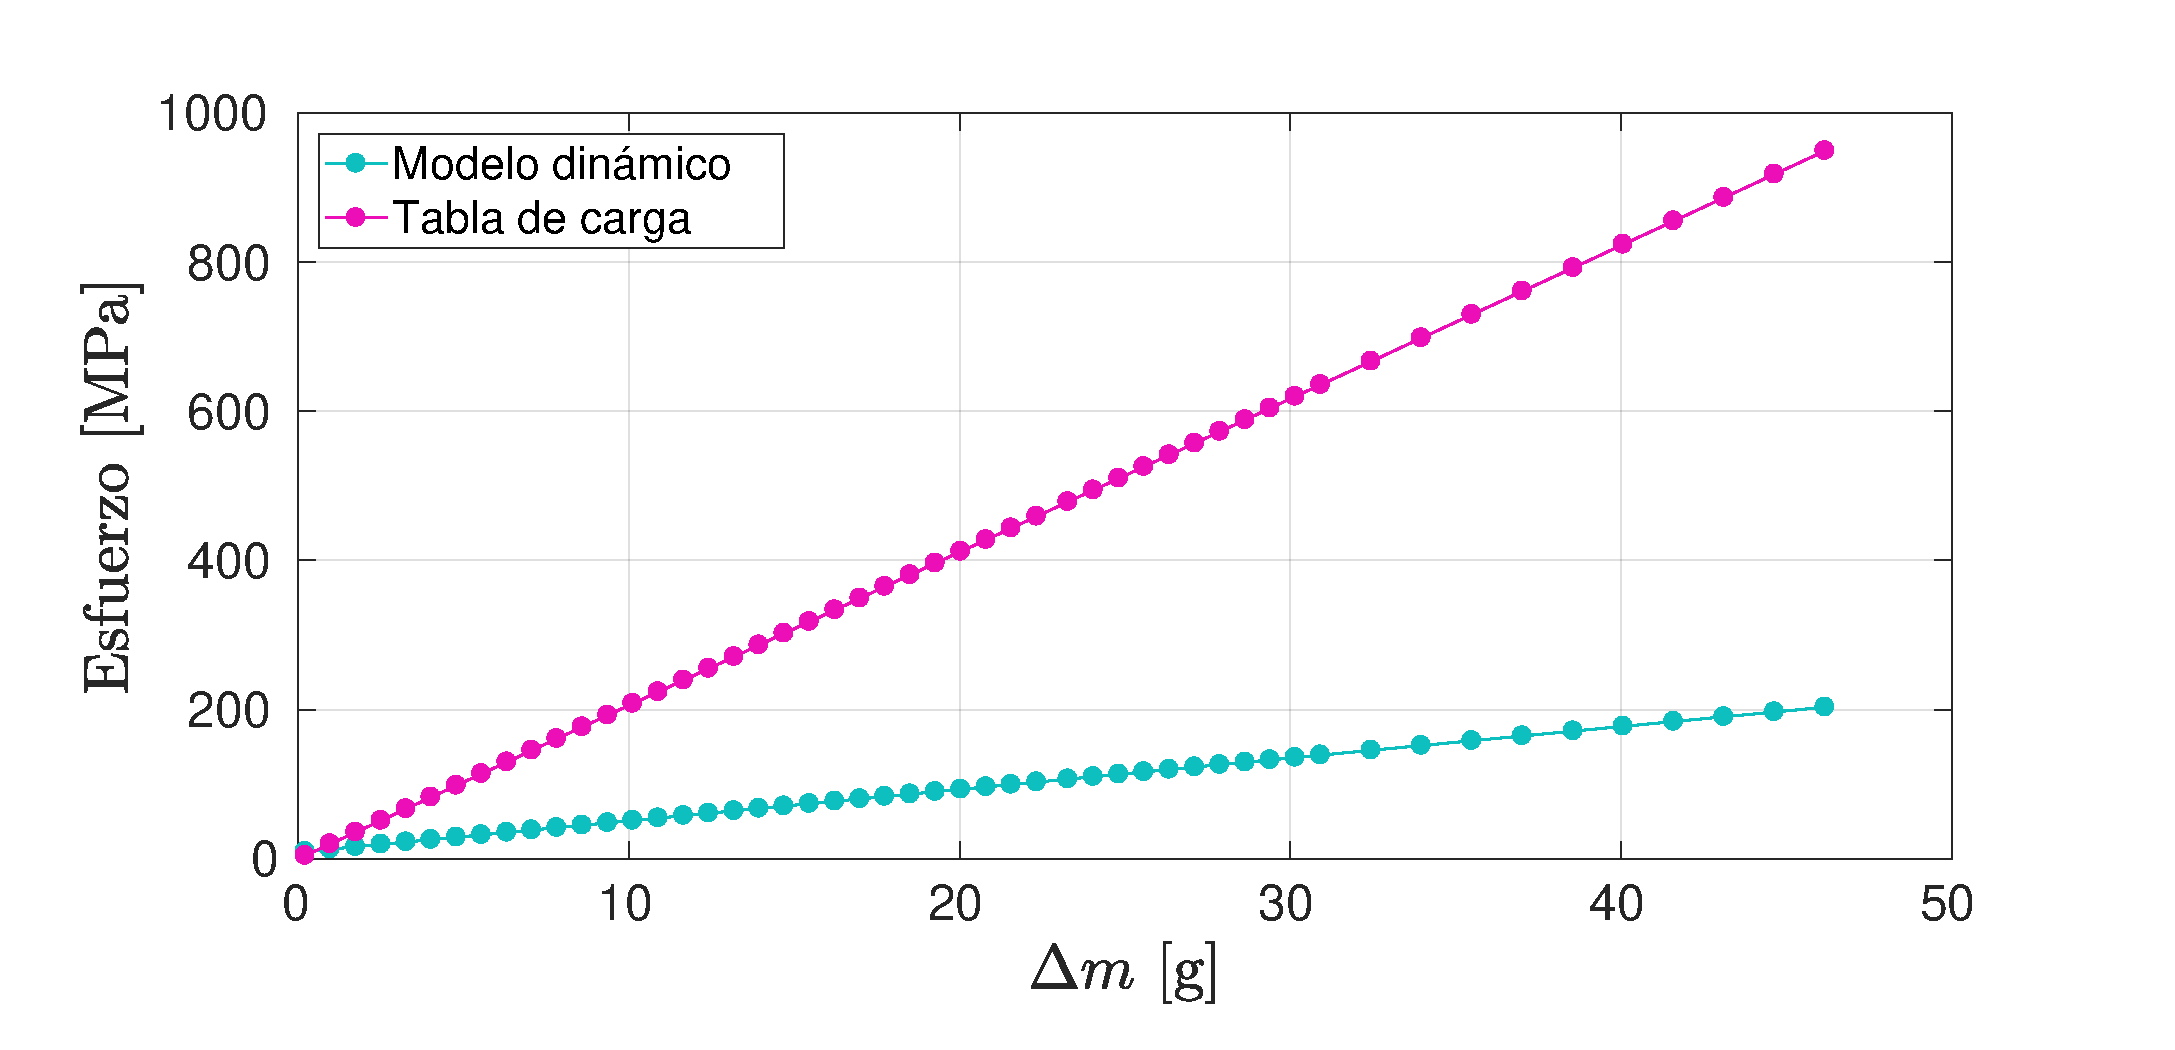
\includegraphics[width=1\linewidth, trim={1cm 0cm 2cm 0cm},clip]{Imagenes/comp_modtab.pdf}
\caption{Comparación entre la curva de esfuerzos $\sigma$ mostrada en la tabla de cargas y el esfuerzo de von Mises $\sigma_{vm}$ del modelo dinámico de acuerdo al contrapeso aplicado $\Delta m$.}
\label{fig:comp_modtab}
\end{figure}

Al realizar un ajuste lineal a los datos, se obtiene que la ecuación para cada fuente de información es:
\begin{align}
	&\text{Modelo dinámico:}& \sigma_{vm} = 2107\cdot \Delta m + 8.496 \\
	&\text{Tabla de carga:} & \sigma = 10282\cdot \Delta m - 0.087 
\end{align}
Por lo tanto, se puede apreciar como la pendiente de la recta de la tabla de carga es casi 5 veces mayor a la obtenida mediante el modelo dinámico. Además, se aprecia como no se incluye la fuerza media en la tabla de carga, al ser el intercepto de la ecuación cercano a cero. De esta forma, se definirá y calculará el error del modelo respecto a la tabla de carga de la siguiente manera:
\begin{equation}
	\text{\% Error} = \frac{10282 - 2107}{2017} \cdot 100\% = 388.0 \%
\end{equation}

\subsection{Determinación de la carga asociada al esfuerzo de fluencia y el esfuerzo último}

Para determinar la carga necesaria para lograr la fluencia y el esfuerzo último de la probeta, se aumenta de manera constante y progresiva la carga $F_{max}$. La fig. \ref{fig:f_step} muestra la distribución de la fuerza a la que se sometió la probeta hasta alcanzar el esfuerzo último ($\sigma_u$), que se encuentran en el anexo \ref{sec:anexob3}.

\begin{figure}[h]
\centering
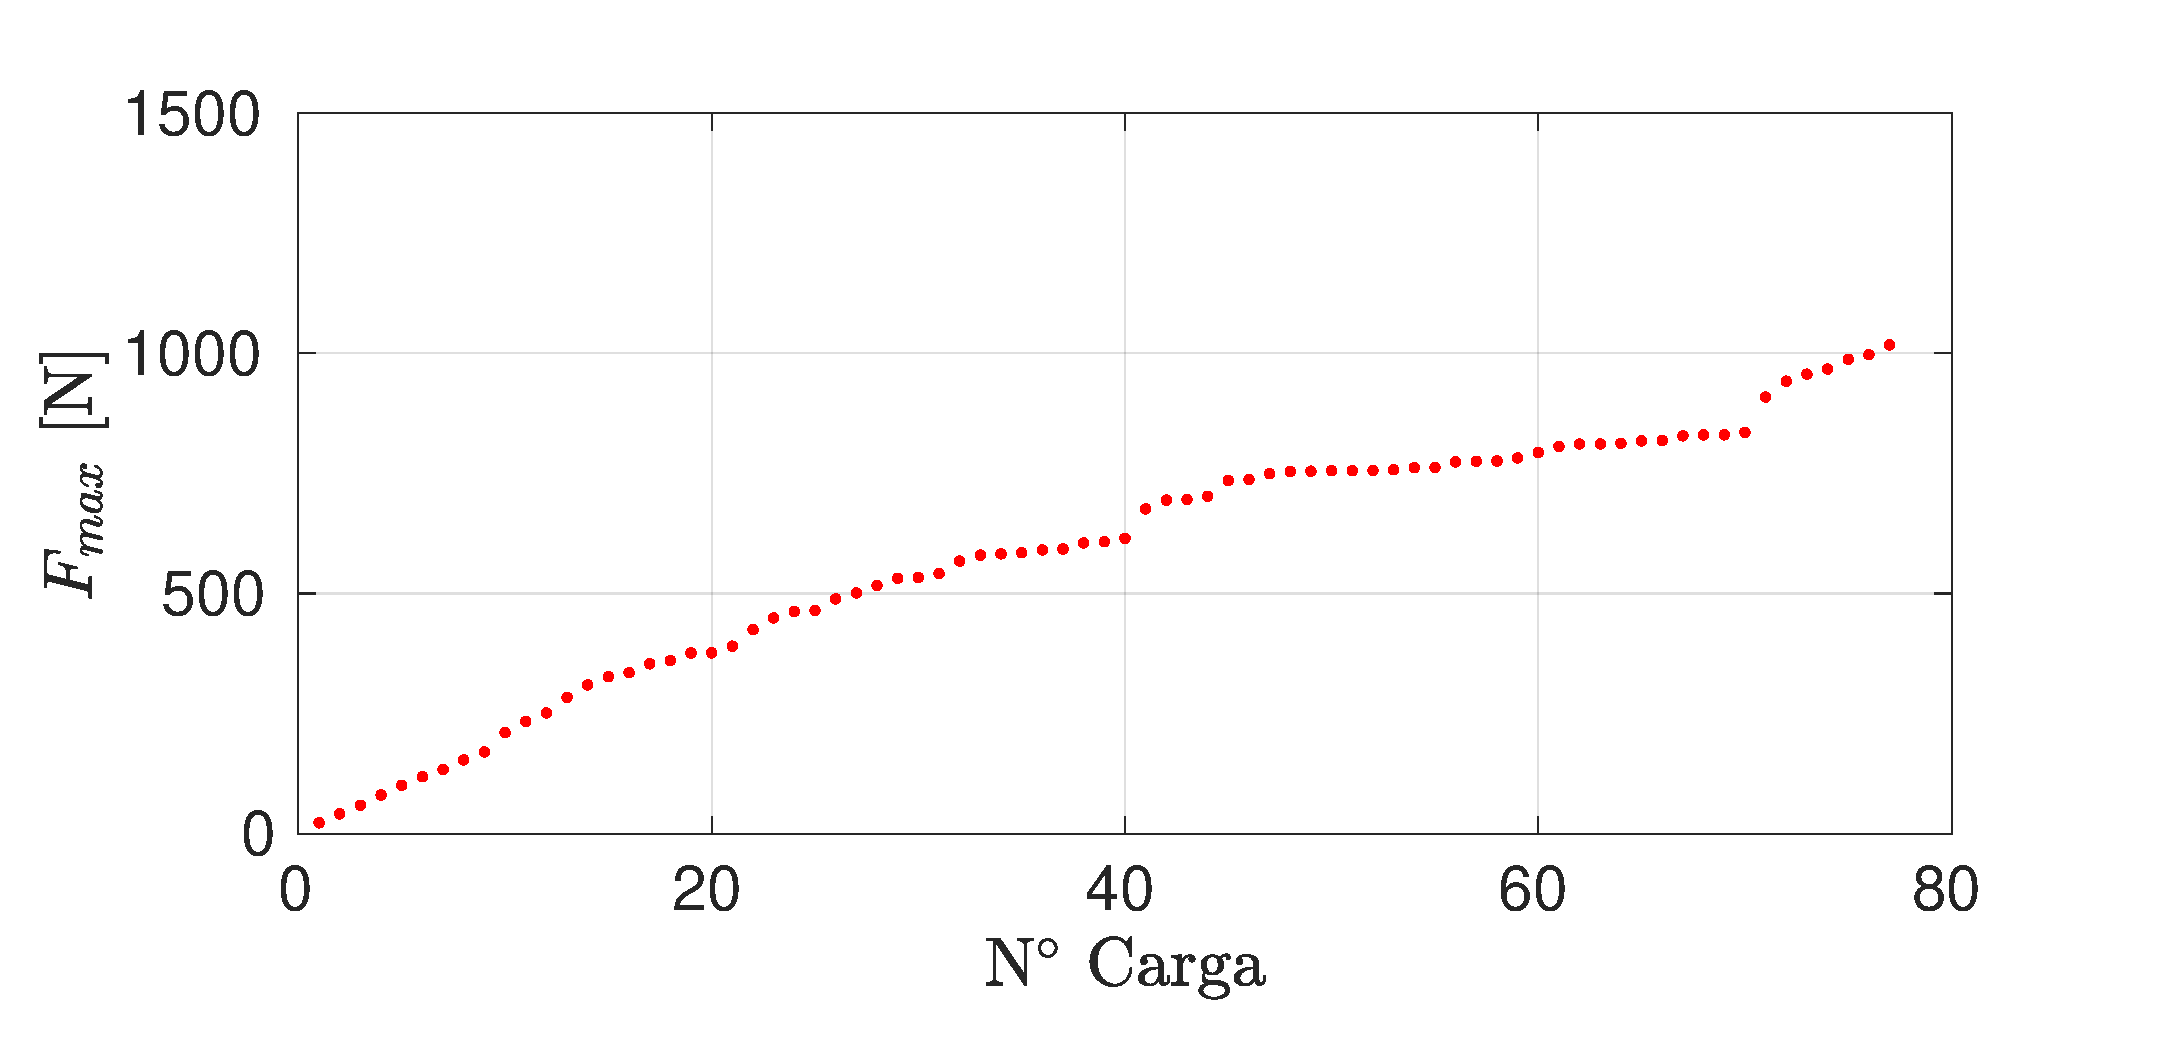
\includegraphics[width=1\linewidth, trim={0cm 0cm 1cm 0cm}, clip]{Imagenes/f_step.pdf}
\caption{Curva de las 76 cargas aplicadas sobre la probeta. Tabla en anexo \ref{sec:anexob3}}
\label{fig:f_step}
\end{figure}

La distribución de esfuerzos es similar a lo que ocurre en el caso anterior al encontrarse los esfuerzos máximos en la zona superior e inferior de la sección transversal de la probeta (puntos $P$ y $R$, según la fig. \ref{fig:diag_pqr2}), como es posible ver en la fig. \ref{fig:resultados_vm}. Sin embargo, a diferencia de lo mostrado anteriormente, en este caso existe deformación plástica al alcanzar la fluencia del material, continuando hasta el punto del esfuerzo último.


\begin{figure}[p]
\centering
	\begin{subfigure}{\linewidth}
		\centering
		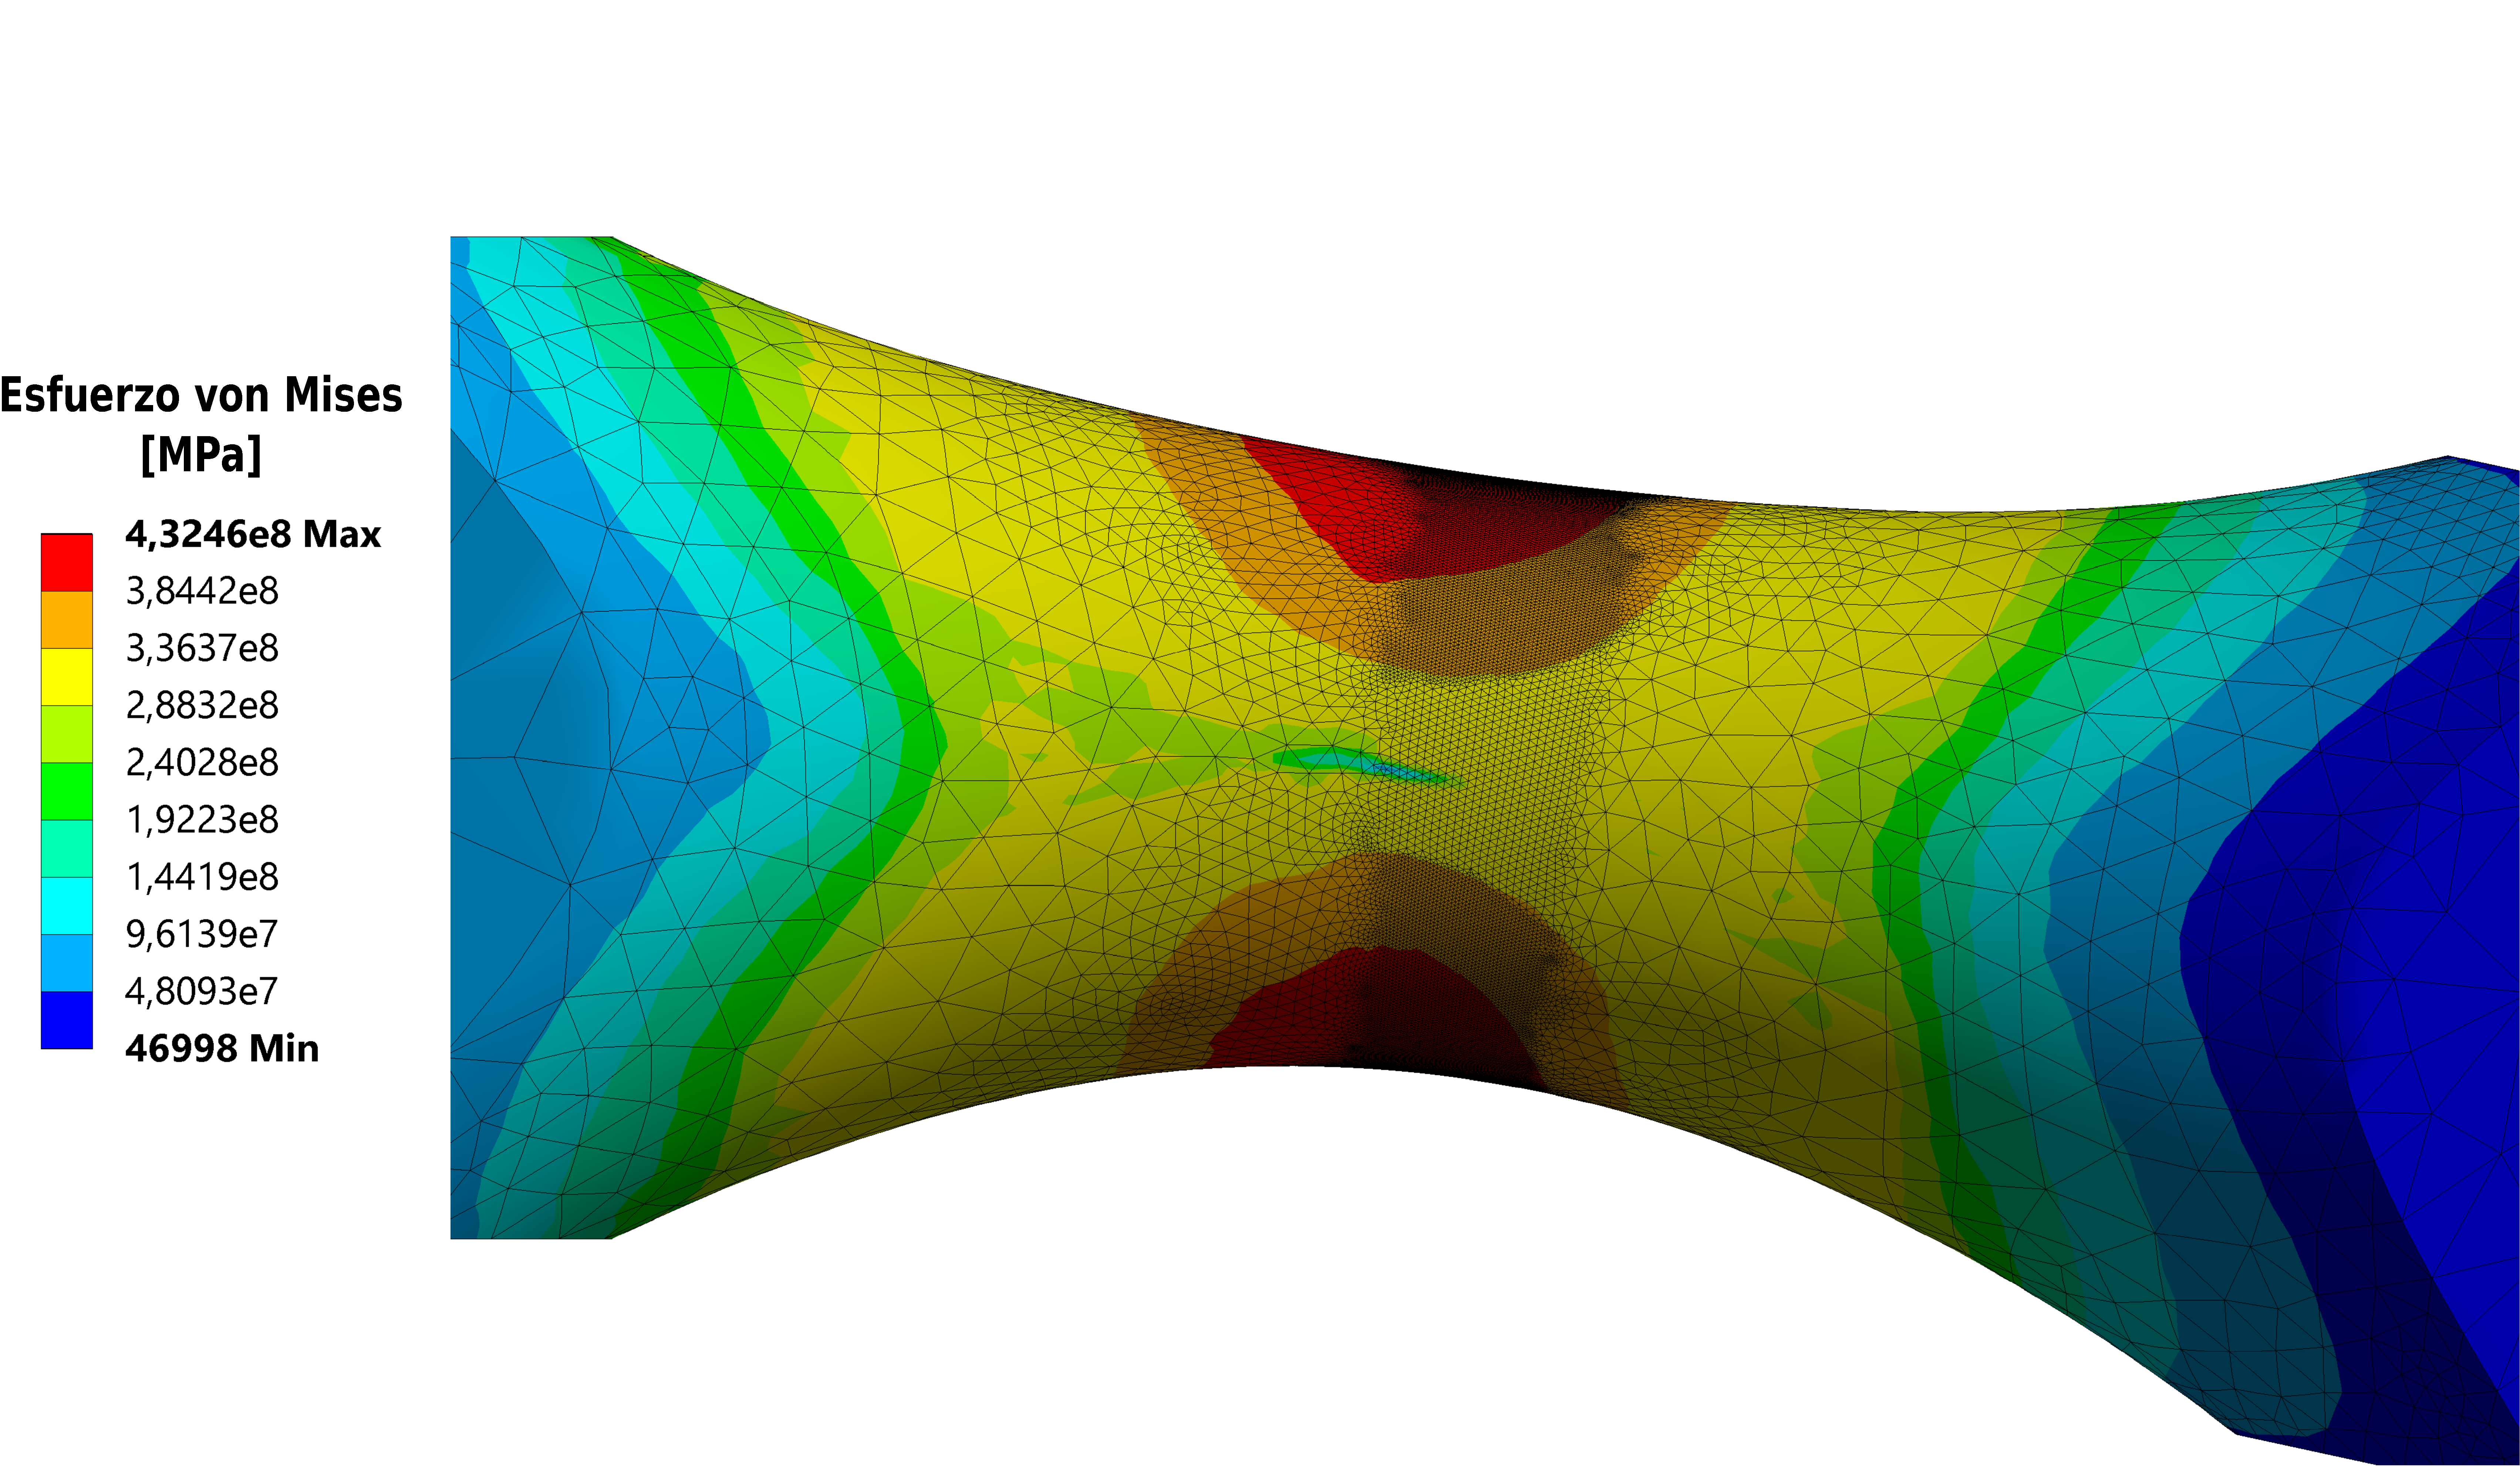
\includegraphics[width=\linewidth]{Imagenes/r_lat.pdf}
		\caption{Vista lateral de la zona intermedia.}
		\label{fig:r_lat}
	\end{subfigure}
	\begin{subfigure}{0.8\linewidth}
		\centering
		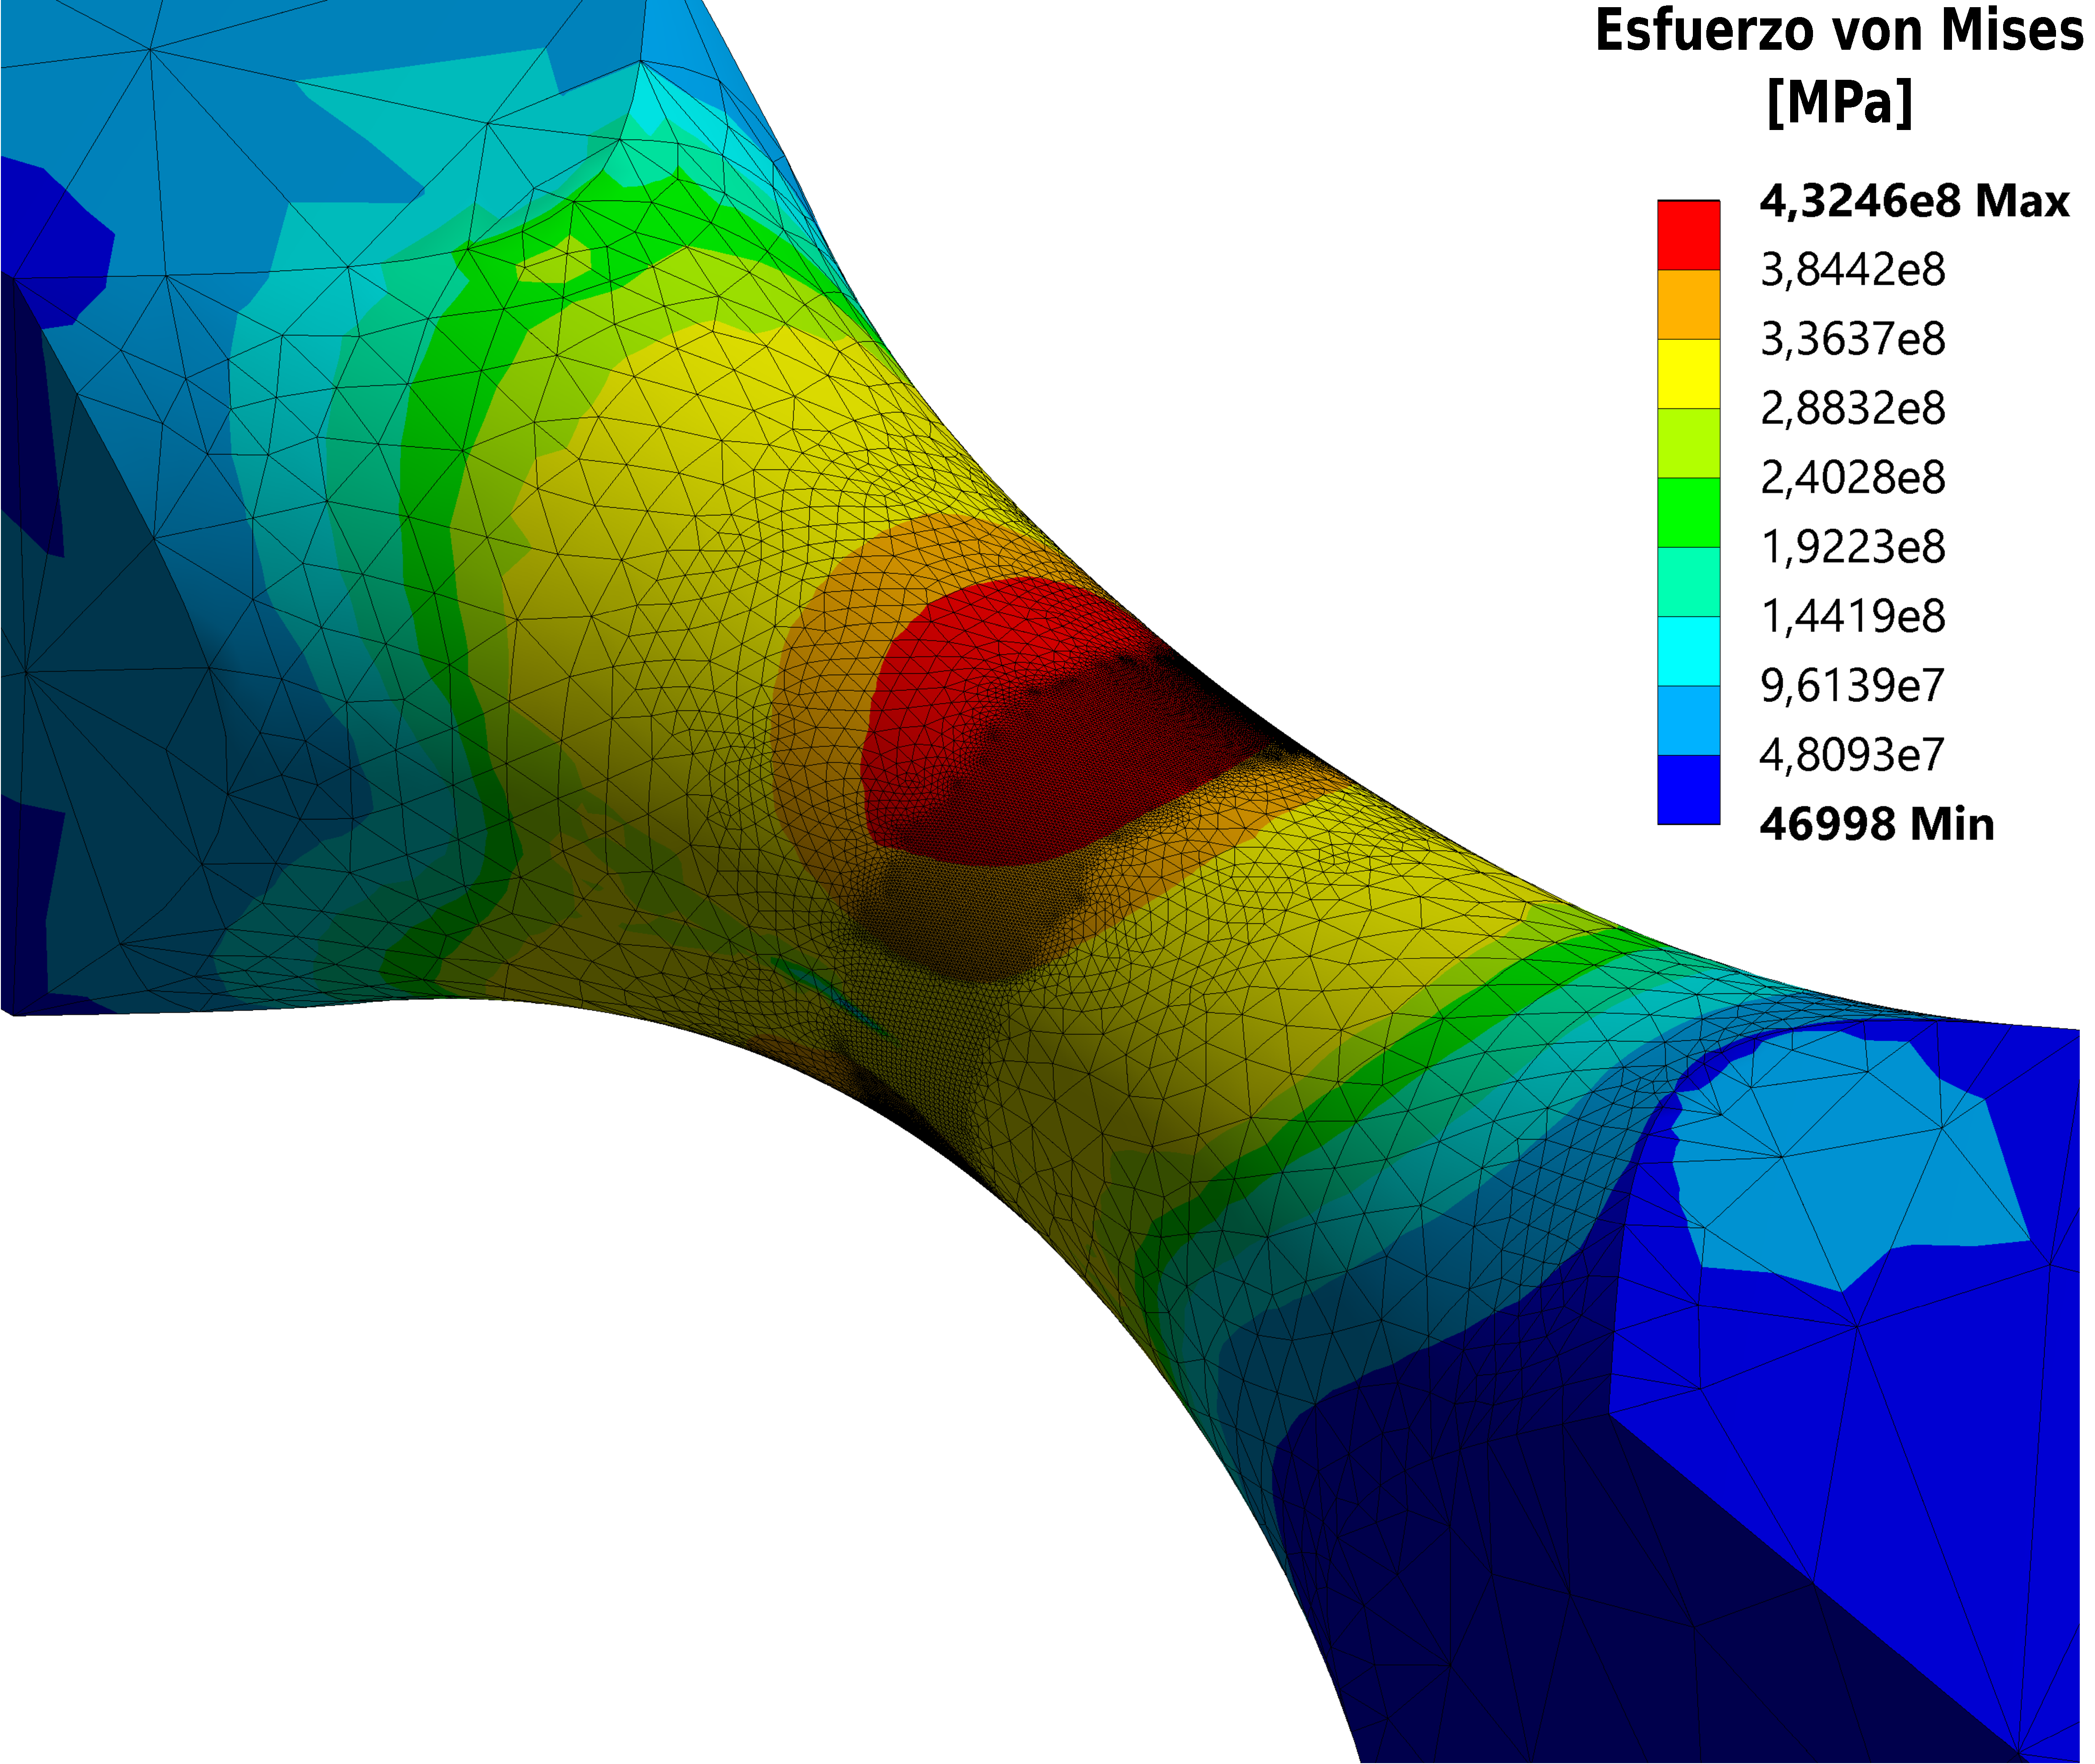
\includegraphics[width=\linewidth]{Imagenes/r_iso.pdf}
		\caption{Vista en isométrico de la zona intermedia.}
		\label{fig:r_iso}
	\end{subfigure}
\end{figure}
\begin{figure}[p]
	\ContinuedFloat
	\centering
	\begin{subfigure}{0.95\linewidth}
		\centering
		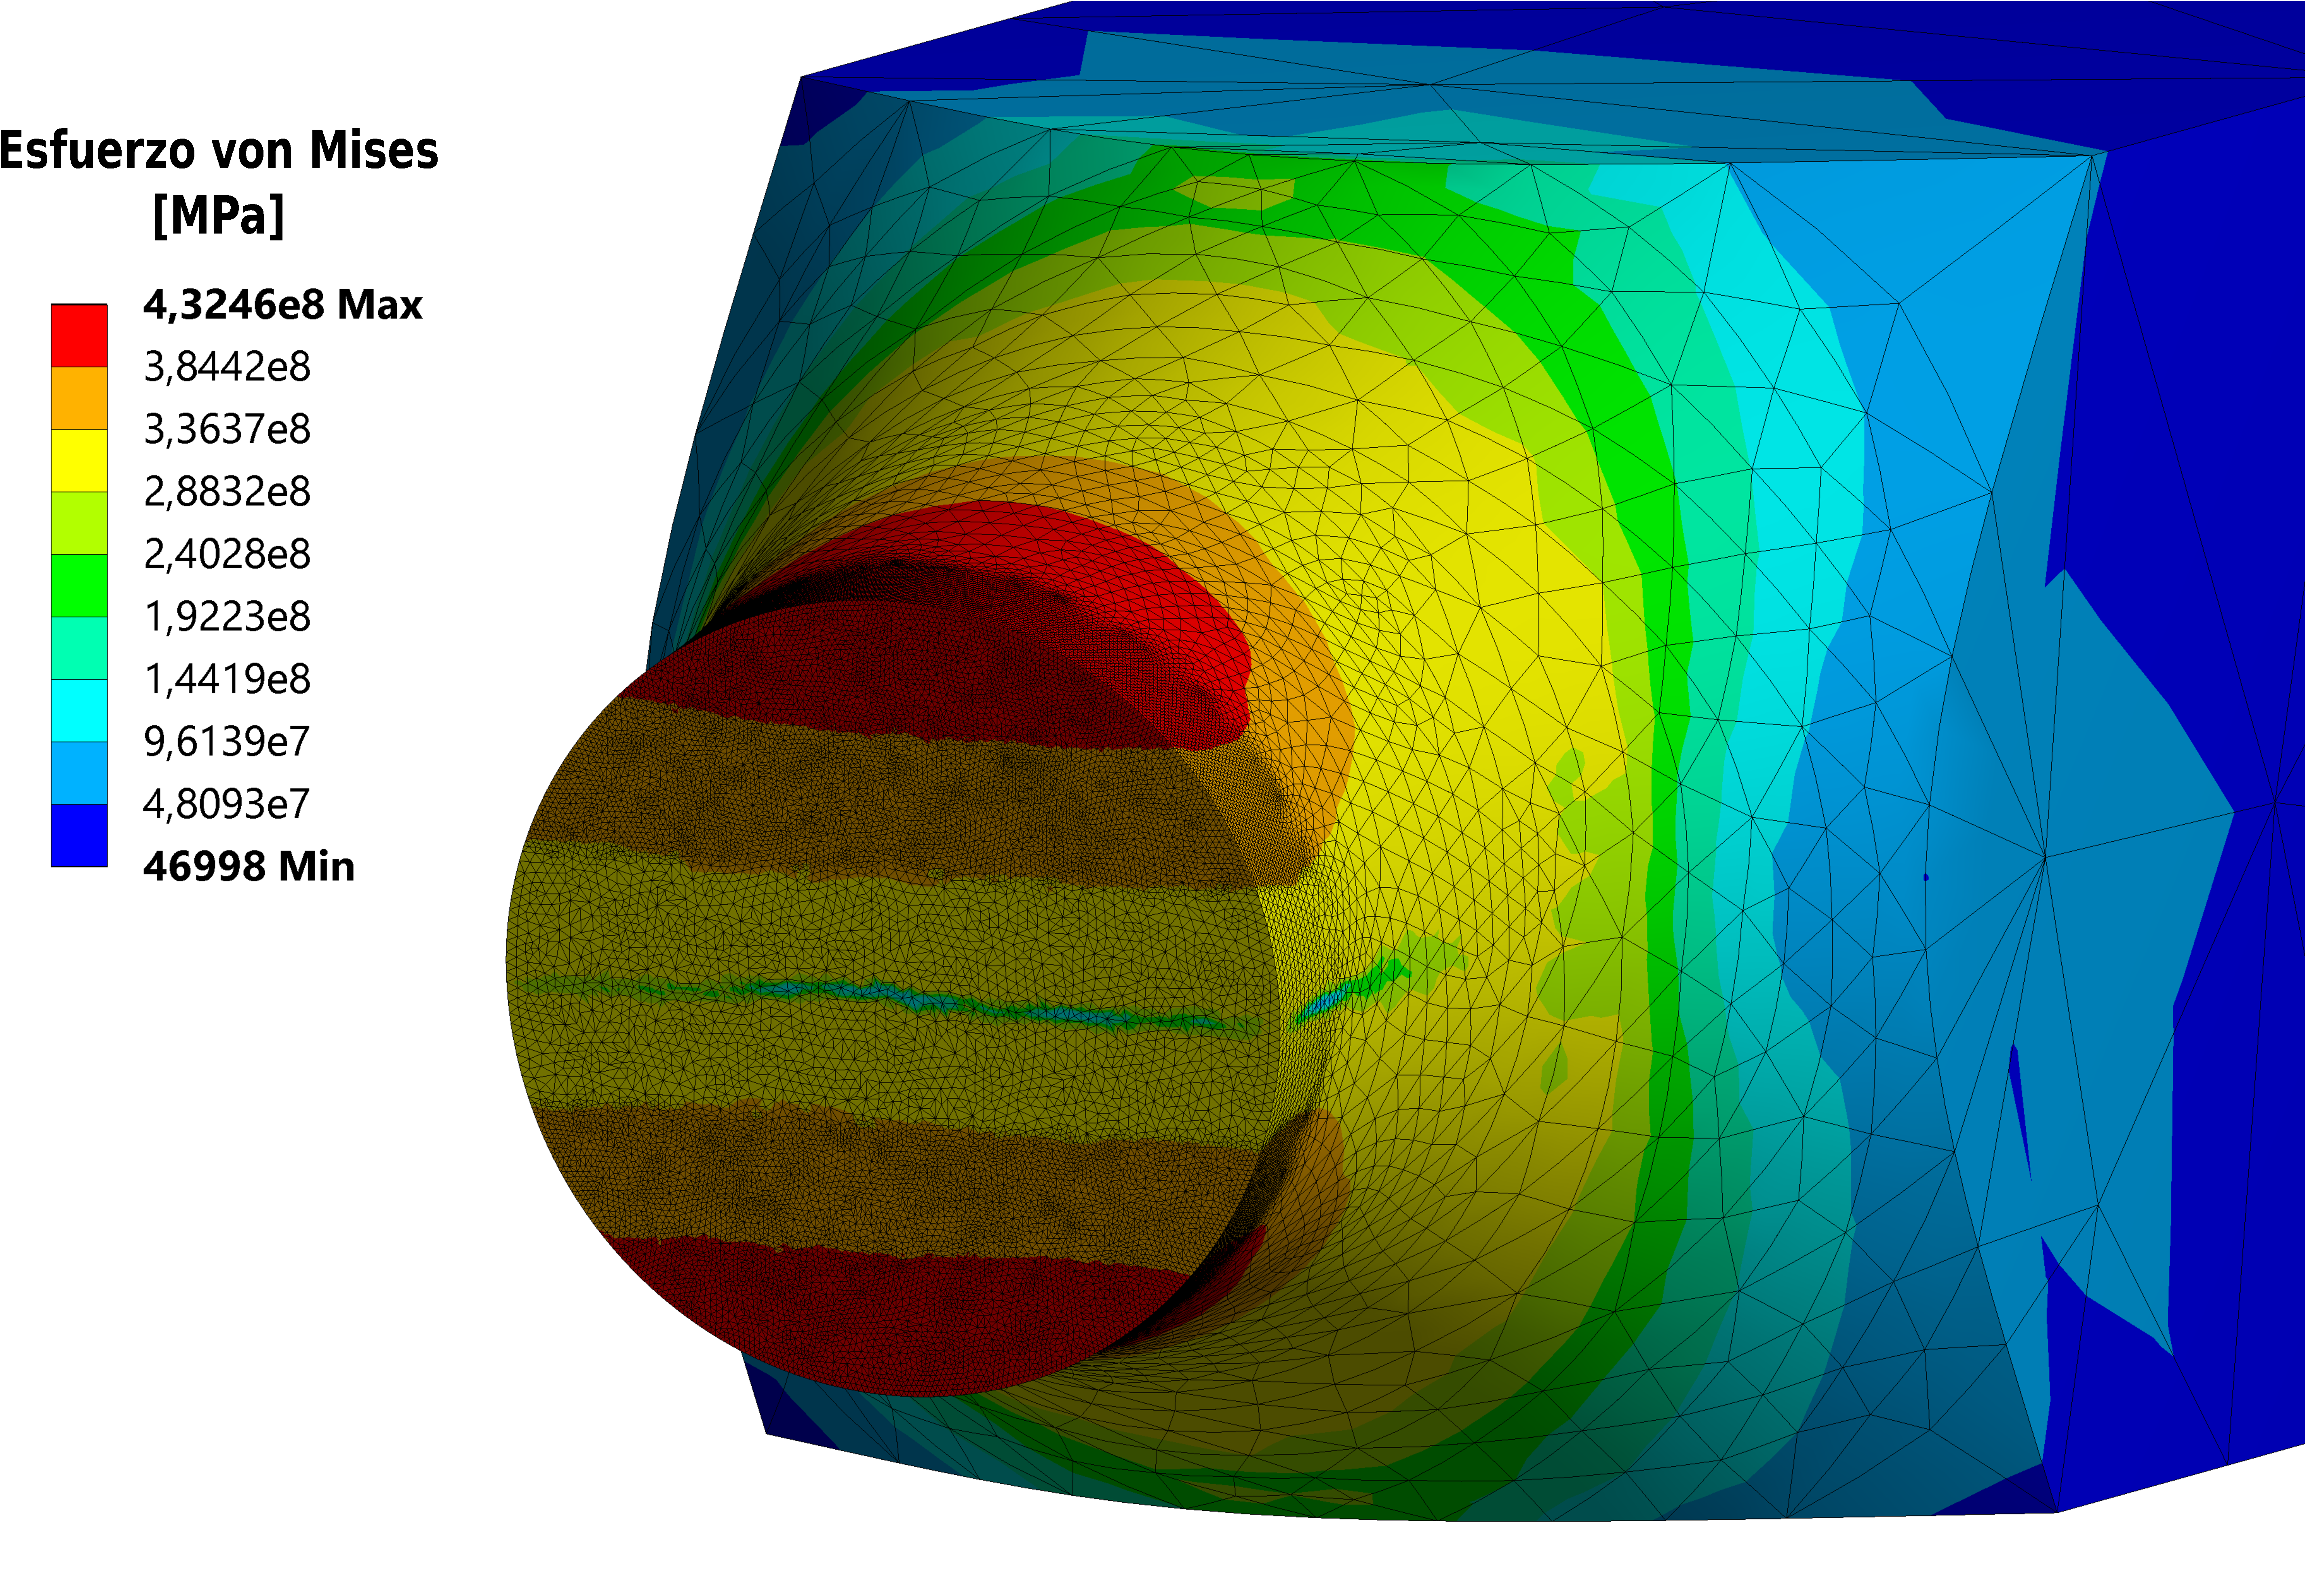
\includegraphics[width=\linewidth]{Imagenes/rcorte_iso.pdf}
		\caption{Vista en isométrico del corte transversal.}
		\label{fig:rcorte_iso}
	\end{subfigure}		
	\begin{subfigure}{0.95\linewidth}
		\centering
		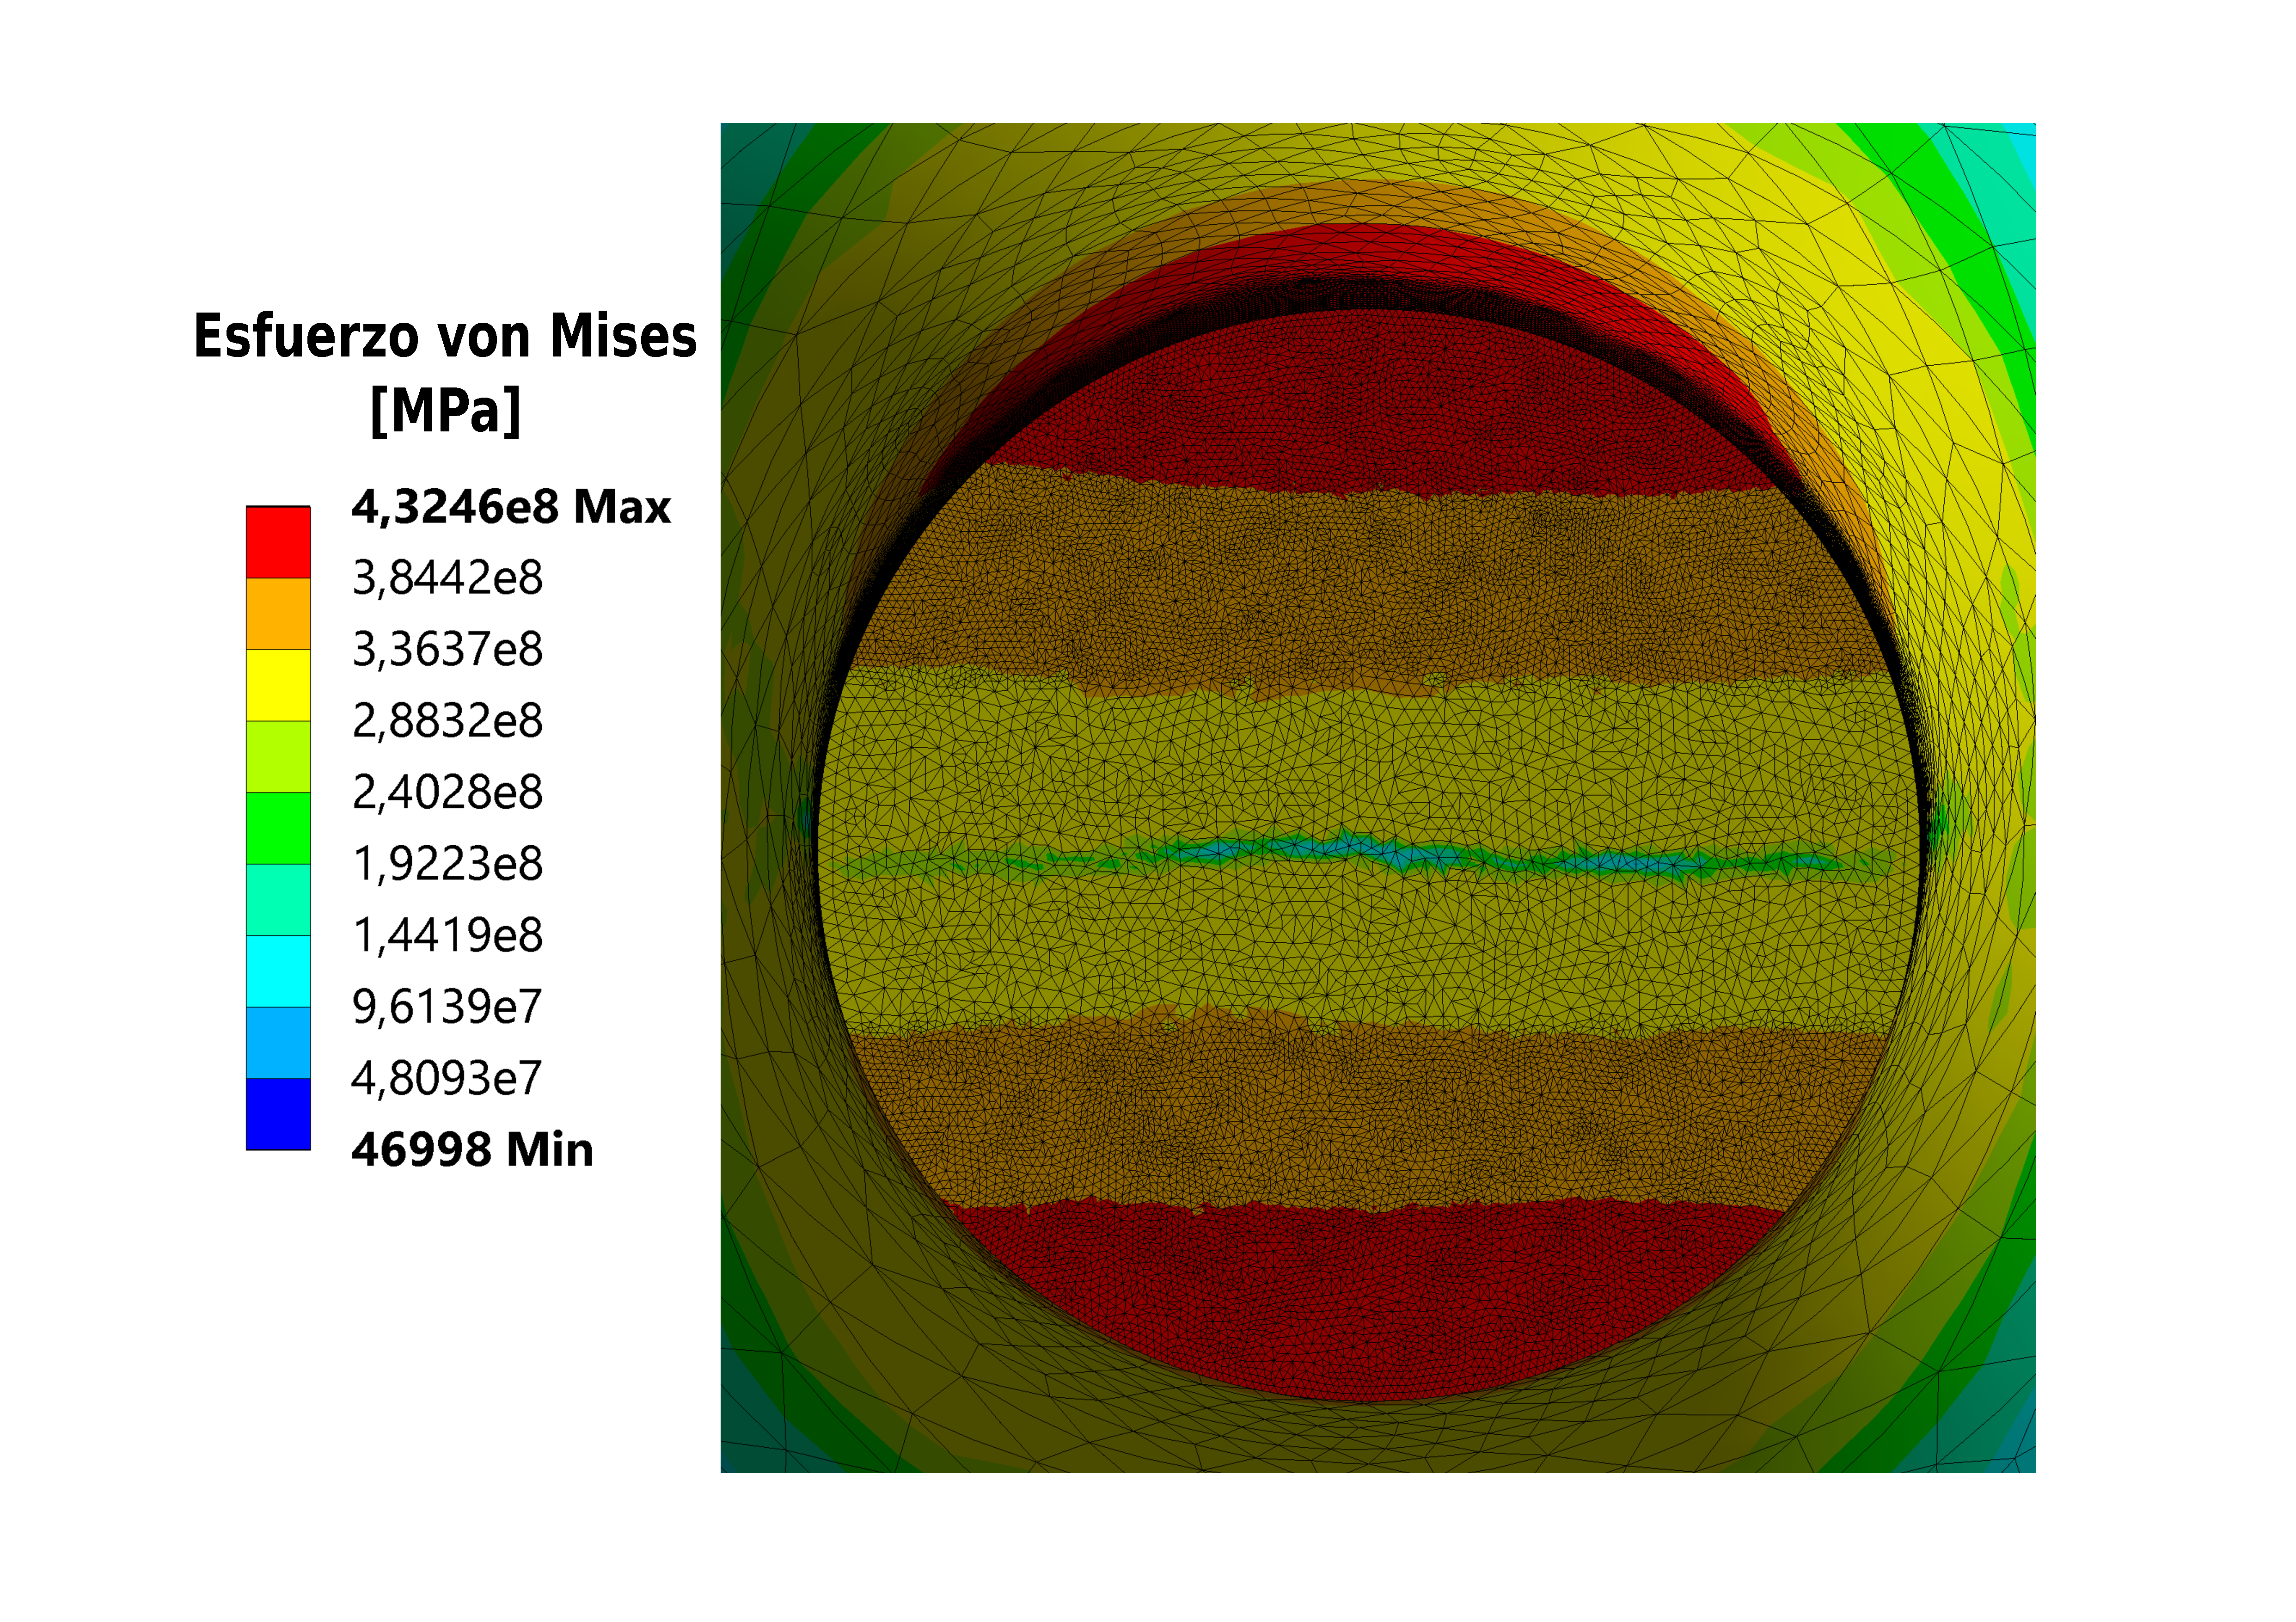
\includegraphics[width=\linewidth]{Imagenes/rcorte.pdf}
		\caption{Vista en detalle del corte transversal.}
		\label{fig:rcorte}
	\end{subfigure}
\caption{Detalle de la distribución de esfuerzos de von Mises en la zona intermedia de la probeta.}
\label{fig:resultados_vm}
\end{figure}

\newpage

\subsection{Identificación de las cargas $\mathbf{F_{max,y}}$ y $\mathbf{F_{max,u}}$}

Para lograr identificar la carga máxima ($F_{max}$) que corresponde al esfuerzo de fluencia y el esfuerzo último, se grafican los resultados de la deformación unitaria normal ($\varepsilon_x$) y de von Mises total ($\varepsilon_{vm,t}$), además de los esfuerzos de von Mises ($\sigma_{vm}$), normal ($\sigma_x$) y cortante máximo ($\tau_{max}$). A partir de las figuras \ref{fig:def_pqr} y \ref{fig:esf_pqr}, se puede apreciar que cuando la fuerza máxima es 450 N (carga n$^{\circ}$ 23) se llega a un esfuerzo de 293,5 MPa, tanto en el punto $P$ como en el punto $R$, alcanzando el esfuerzo de fluencia del material. Además, se puede identificar que el esfuerzo último se alcanza con la carga n$^{\circ}$ 76 de 1000 N.

En contraste, el punto $Q$ alcanza el punto de fluencia de forma tardía, específicamente en la carga n$^{\circ}$ 68 de 830,2 N, sin llegar hasta el esfuerzo último. Respecto a este mismo punto, se aprecia como los esfuerzos normales $\sigma_x$ son cercanos a cero, como es esperable al encontrarse en el eje neutro, sin embargo, cuando la deformación plástica aumenta de manera significativa, se ve que el punto $Q$ comienza a sufrir esfuerzos de tracción como consecuencia de salirse del eje neutro de la probeta. Por otra parte, cuando la carga aplicada alcanza los 836 N (carga n$^{\circ}$ 69) se puede apreciar una inestabilidad geométrica en el punto $Q$, que destaca principalmente en la fig. \ref{fig:esfpqr_ms} del esfuerzo cortante máximo. 

Para poner en perspectiva la carga, el desplazamiento de la probeta con dirección al eje $y$ al alcanzar la fluencia y el esfuerzo último corresponde a 0,255 mm y 8,311 mm, respectivamente. A partir del análisis realizado, se puede concluir que la carga máxima para la fluencia de la probeta corresponde a $F_{max,y} = 450$ N y para el esfuerzo último es $F_{max,u} = 1000$ N.

\begin{figure}[p]
\centering
	\begin{subfigure}{1\linewidth}
		\centering
		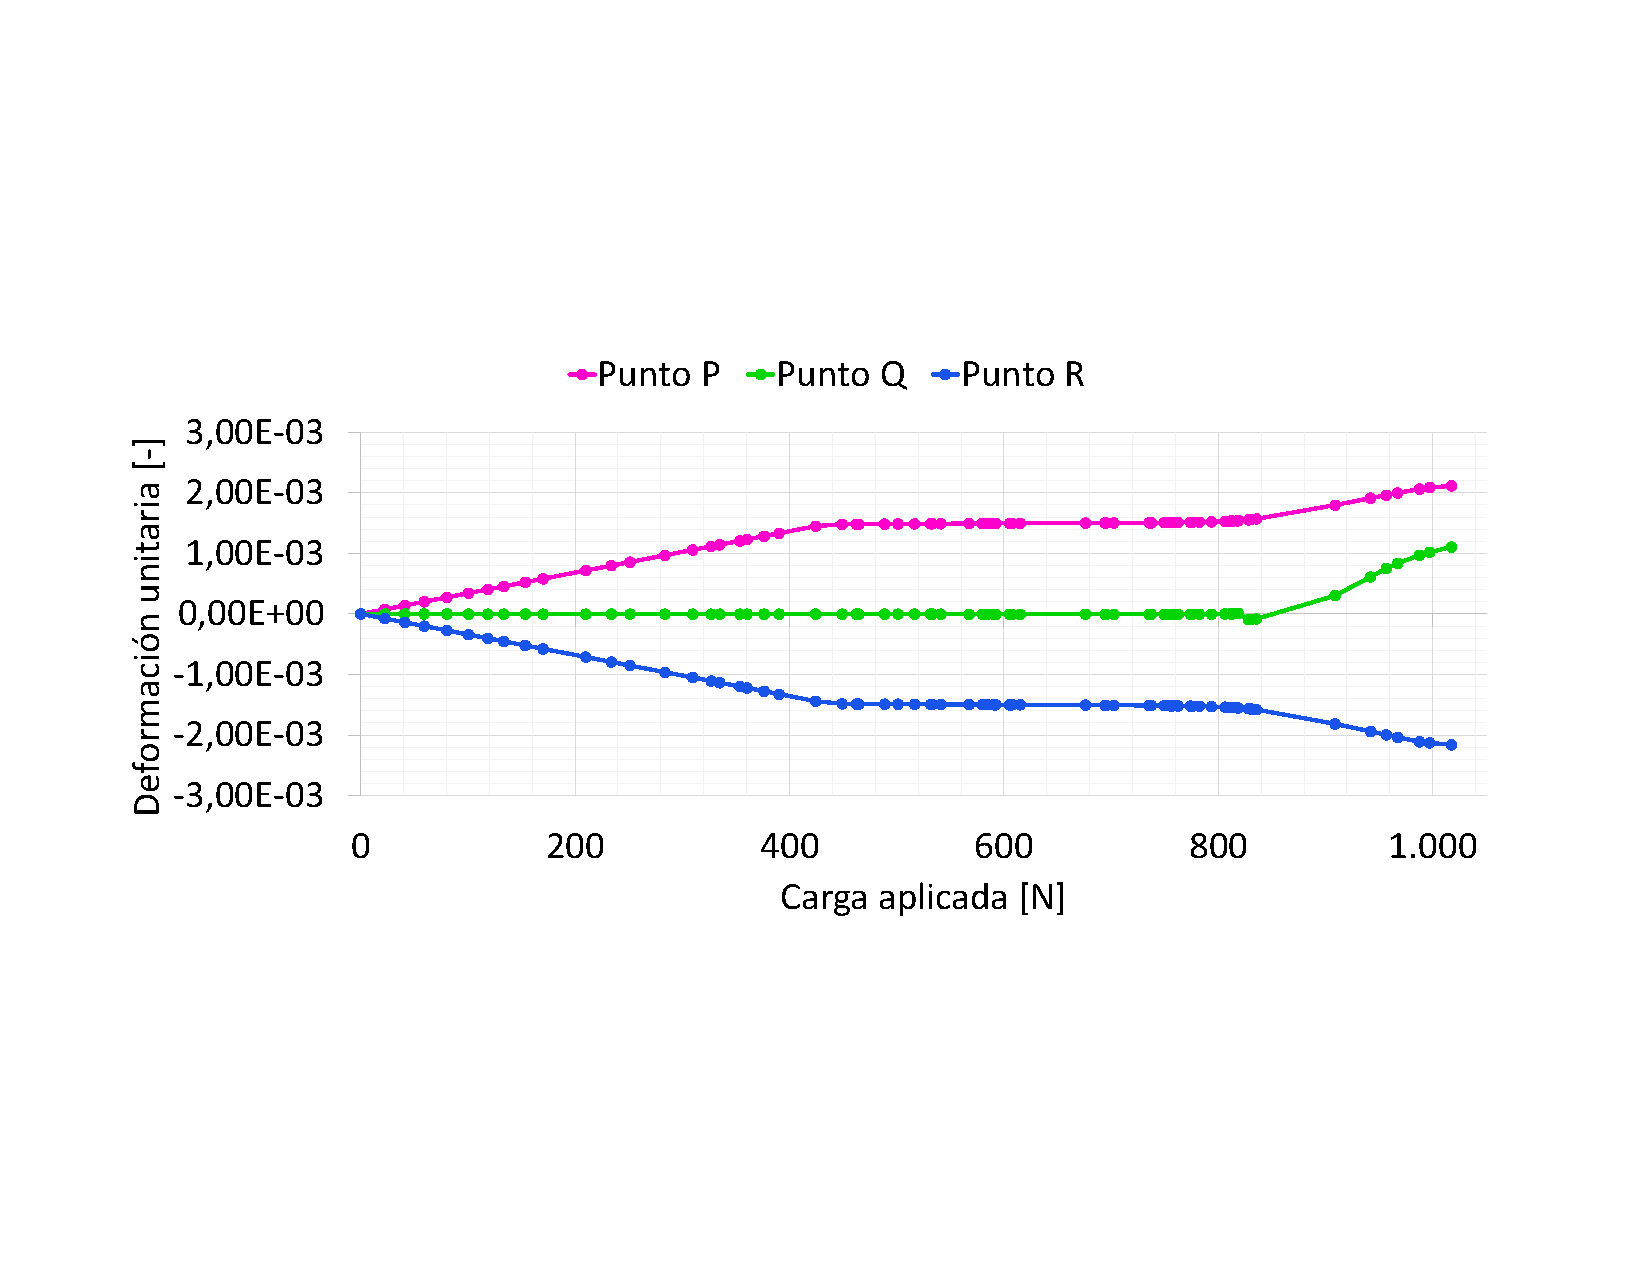
\includegraphics[width=\linewidth, trim={2cm 5cm 2cm 5cm},clip]{Imagenes/defpqr_normal.pdf}
		\caption{Deformación normal, en dirección $x$, de los puntos $P$, $Q$ y $R$.}
		\label{fig:defpqr_normal}
	\end{subfigure}
		\begin{subfigure}{1\linewidth}
		\centering
		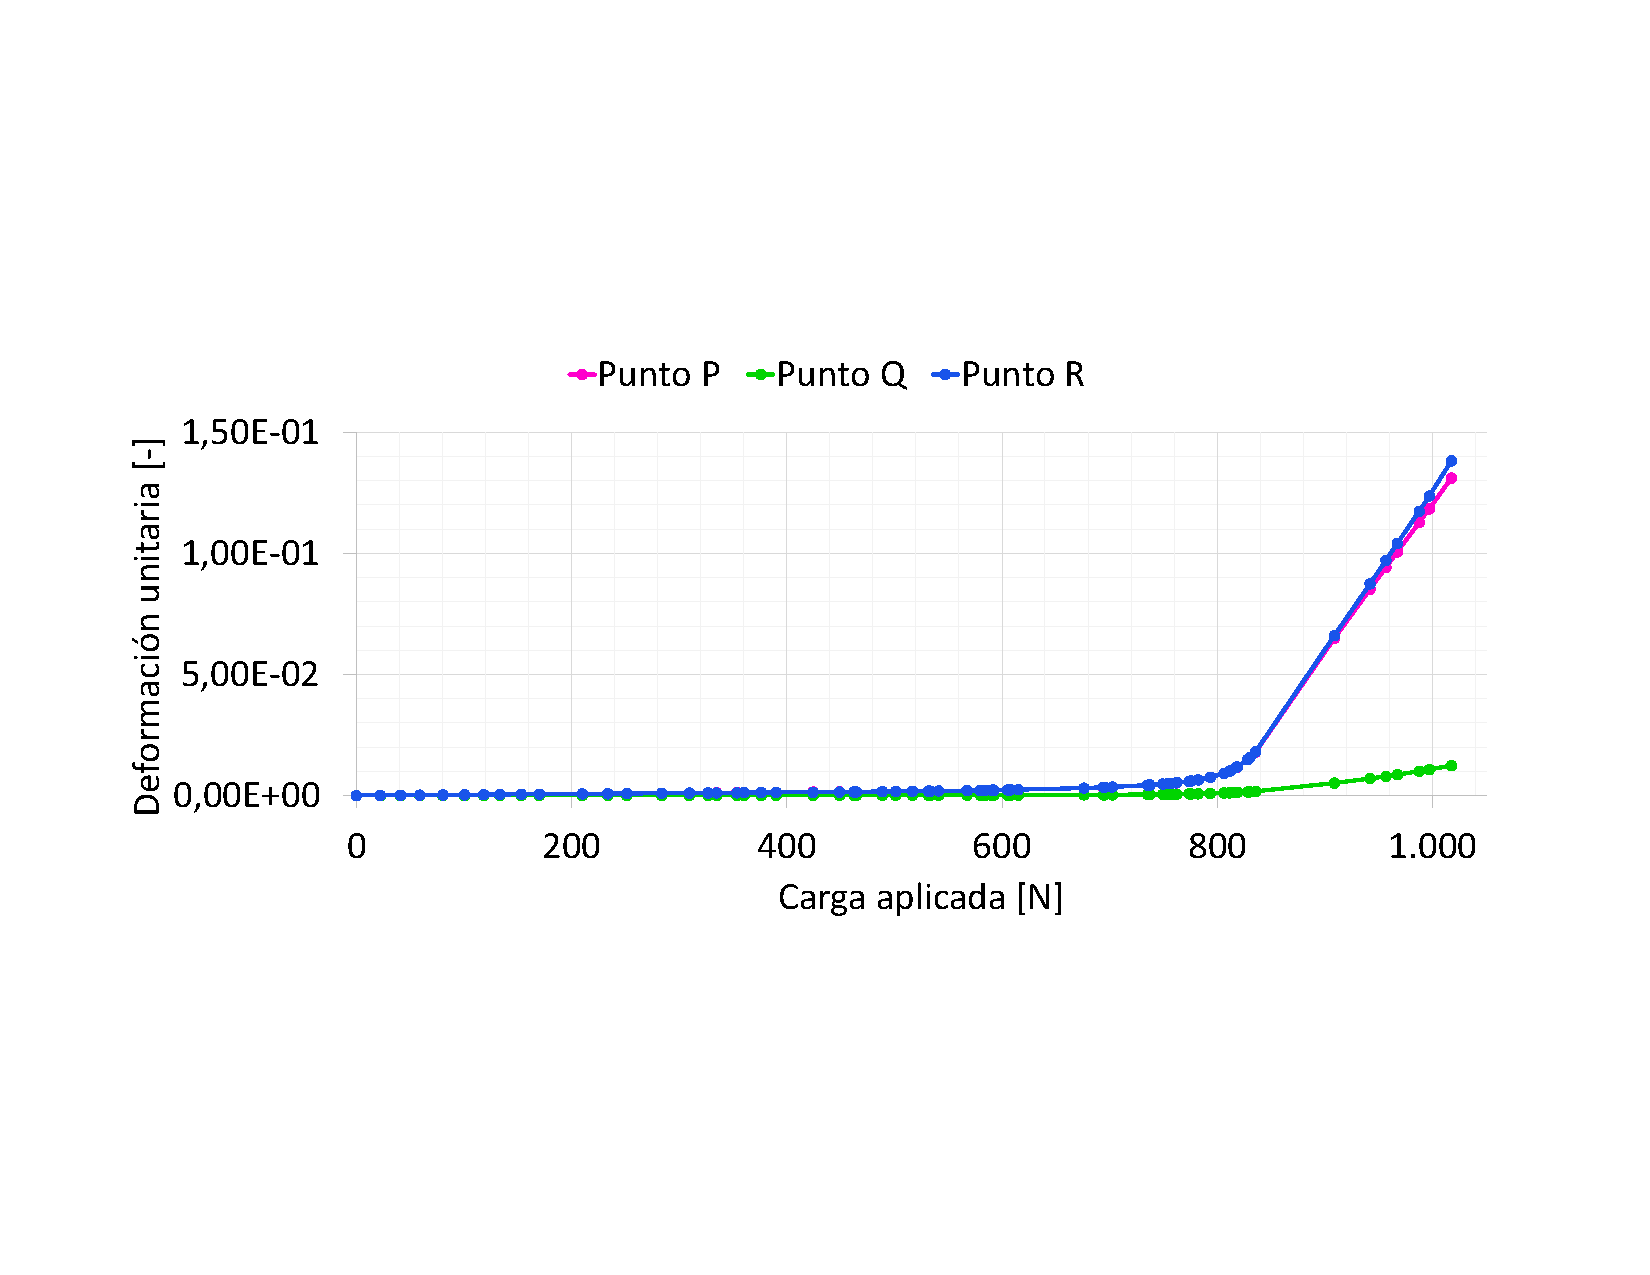
\includegraphics[width=\linewidth, trim={2cm 5cm 2cm 5cm},clip]{Imagenes/defpqr_vmt.pdf}
		\caption{Deformación equivalente total de los puntos $P$, $Q$ y $R$.}
		\label{fig:defpqr_vmt}
	\end{subfigure}
\caption{Deformación unitaria de los puntos $P$, $Q$ y $R$  }
\label{fig:def_pqr}
\end{figure}

\begin{figure}[p]
\centering
	\begin{subfigure}{1\linewidth}
		\centering
		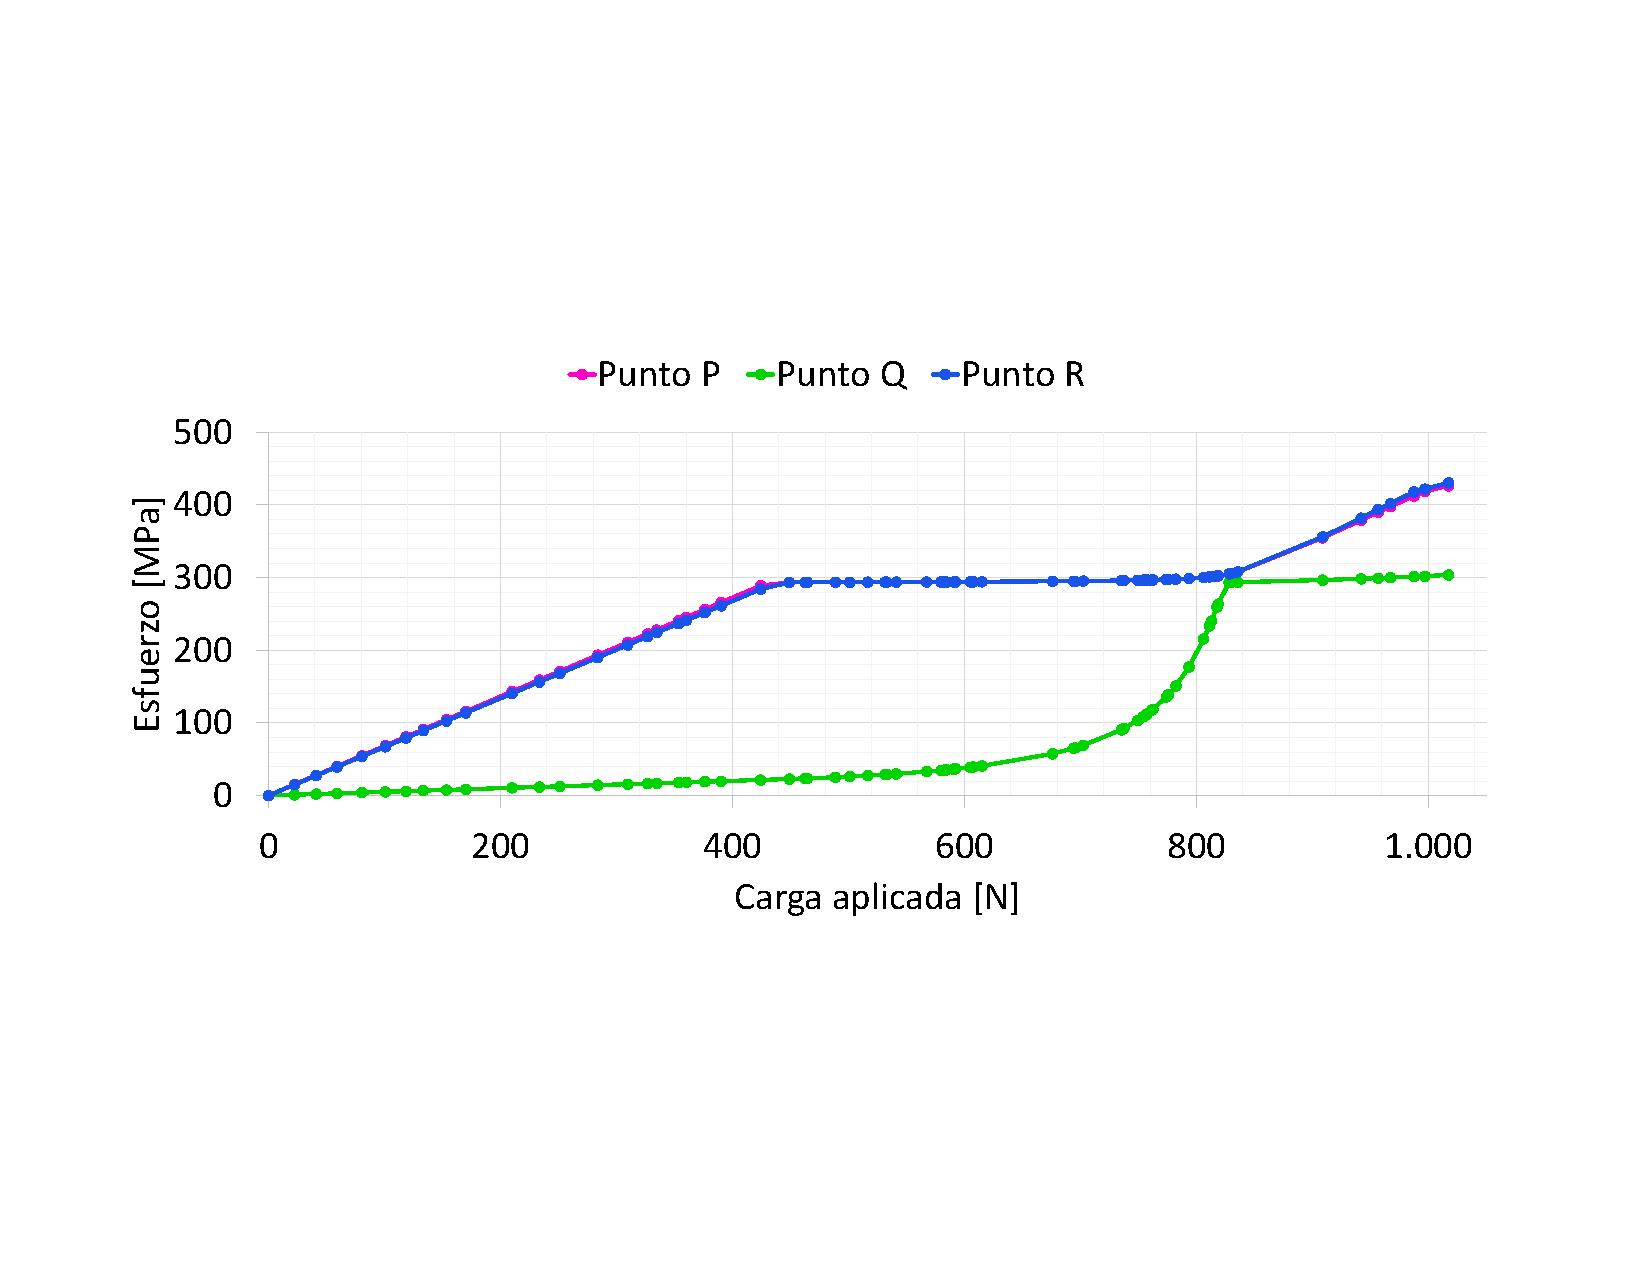
\includegraphics[width=\linewidth, trim={2cm 5cm 2cm 5cm},clip]{Imagenes/esfpqr_vm.pdf}
		\caption{Esfuerzo de von Mises de los puntos $P$, $Q$ y $R$.}
		\label{fig:esfpqr_vm}
	\end{subfigure}
	\begin{subfigure}{1\linewidth}
		\centering
		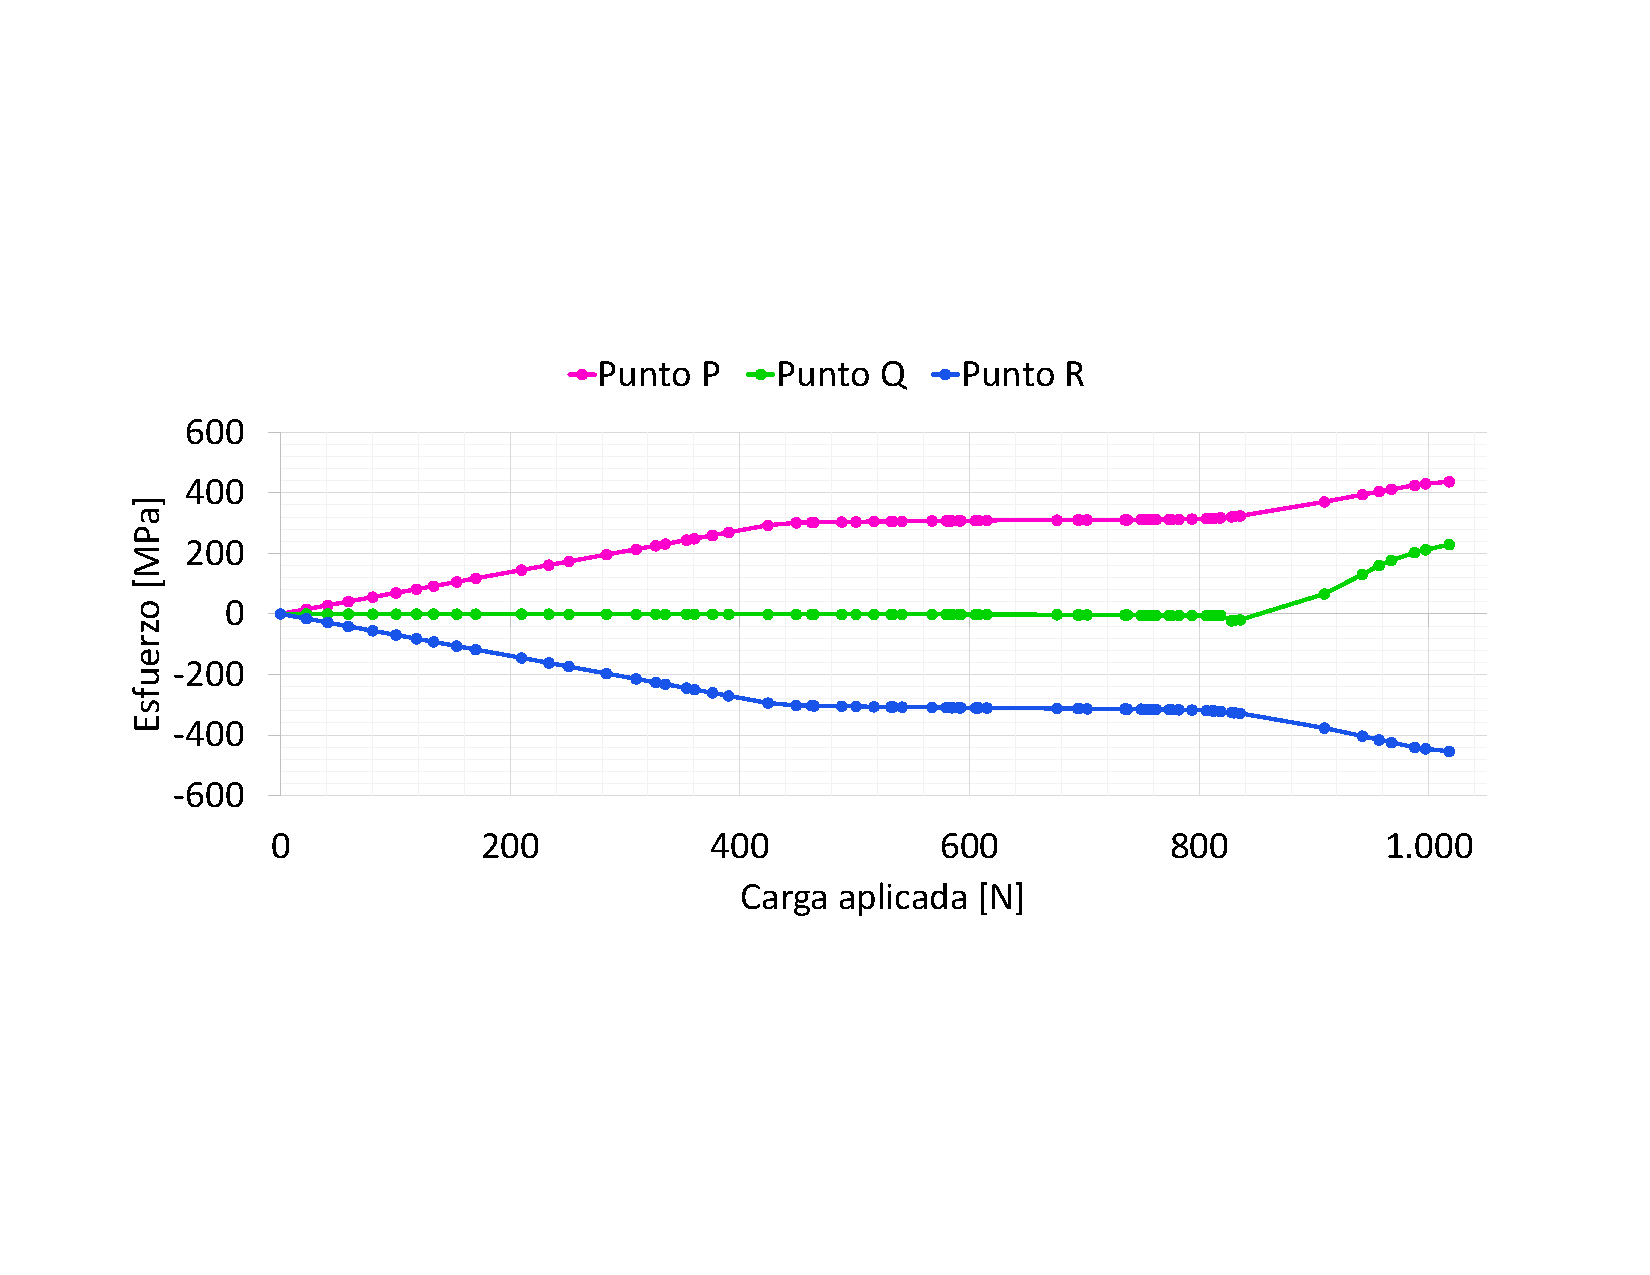
\includegraphics[width=\linewidth, trim={2cm 5cm 2cm 5cm},clip]{Imagenes/esfpqr_normal.pdf}
		\caption{Esfuerzo normal, en dirección $x$, de los puntos $P$, $Q$ y $R$.}
		\label{fig:esfpqr_normal}
	\end{subfigure}
	\begin{subfigure}{1\linewidth}
		\centering
		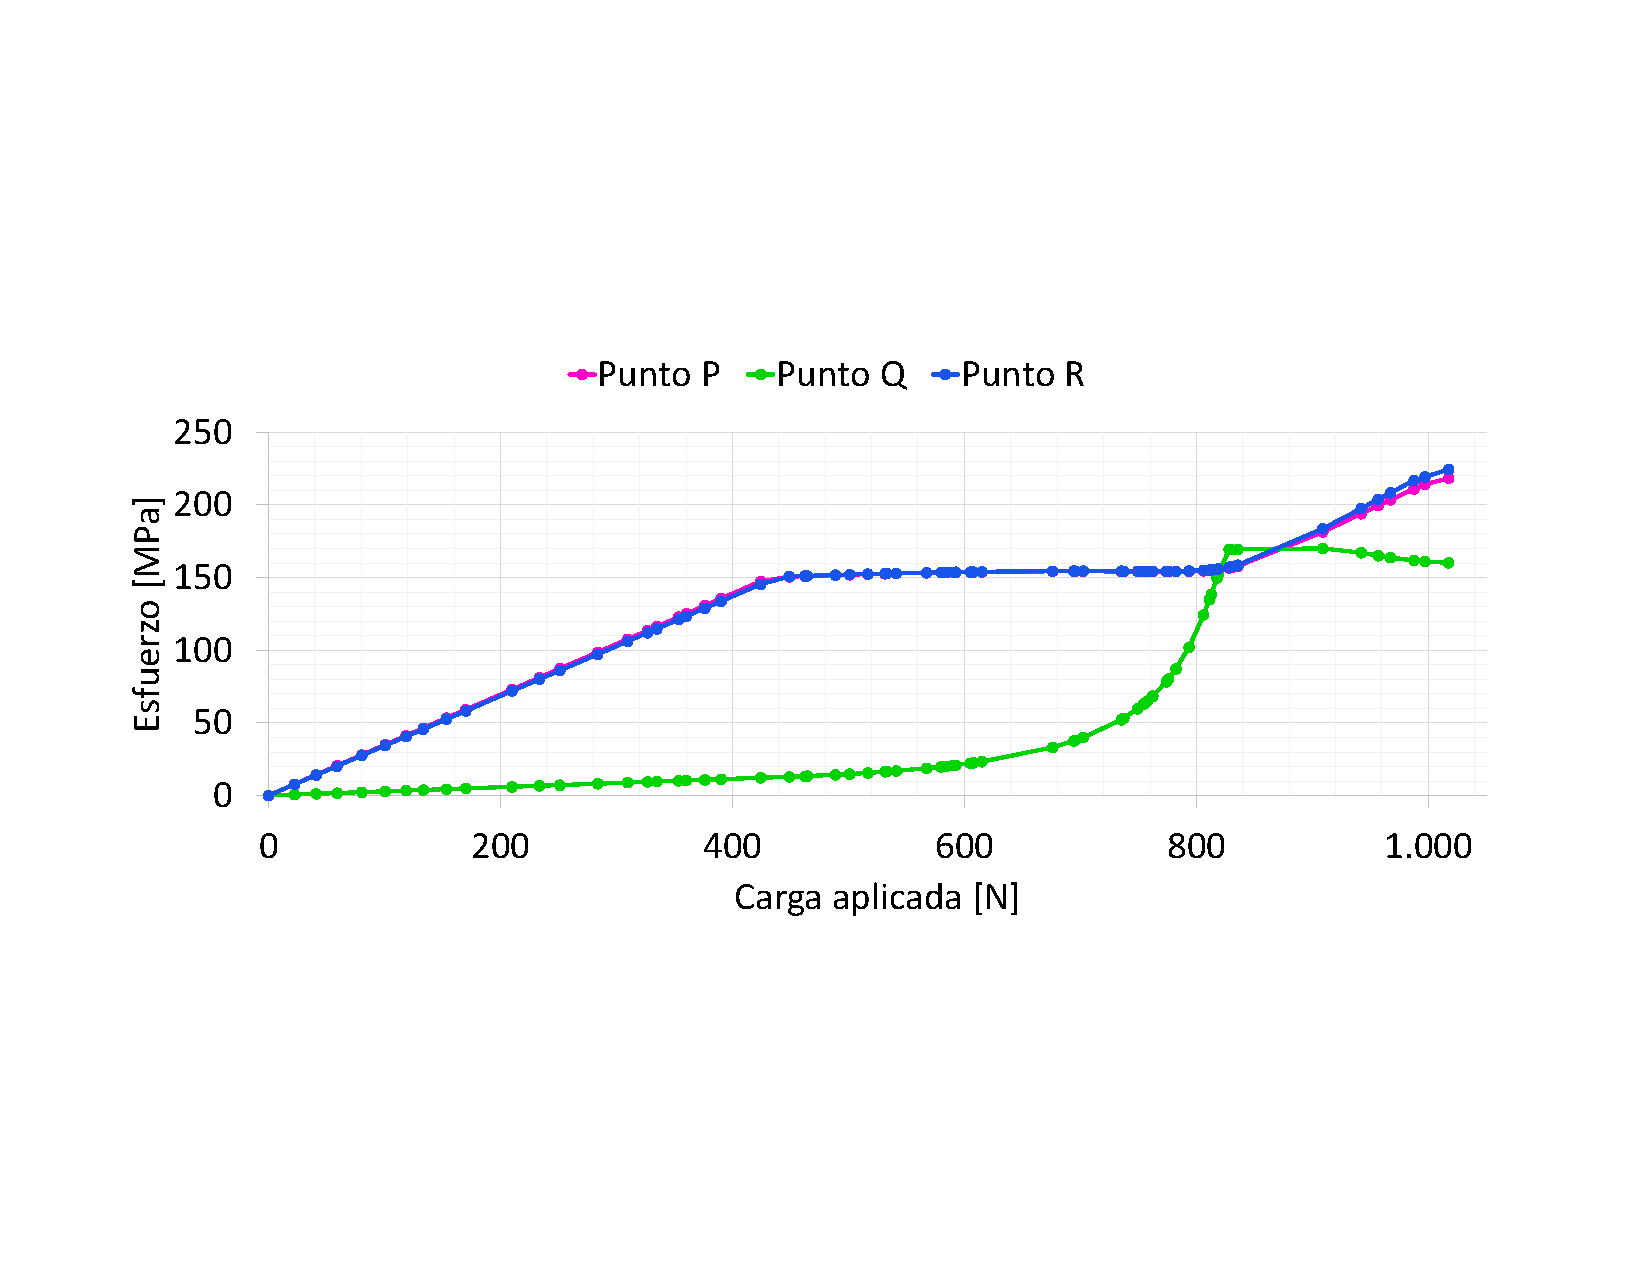
\includegraphics[width=\linewidth, trim={2cm 5cm 2cm 5cm},clip]{Imagenes/esfpqr_ms.pdf}
		\caption{Esfuerzo cortante absoluto de los puntos $P$, $Q$ y $R$.}
		\label{fig:esfpqr_ms}
	\end{subfigure}
\caption{Esfuerzos de von Mises, normal y máximo cortante de los puntos $P$, $Q$ y $R$.}
\label{fig:esf_pqr}
\end{figure}

\newpage

\subsection{Determinación $\mathbf{\Delta m}$ para la carga máxima $\mathbf{F_{max,y}}$ y $\mathbf{F_{max,u}}$}

Para encontrar la masa $\Delta m$ necesaria para realizar las cargas $F_{max,y}$ y $F_{max,u}$ se hará un ajuste lineal sobre los datos que se obtuvieron a partir del modelo, para una velocidad $\omega_{max}= 1500$ rpm, como se puede ver en la fig. \ref{fig:fmax_dmec}.

\begin{figure}[h]
\centering
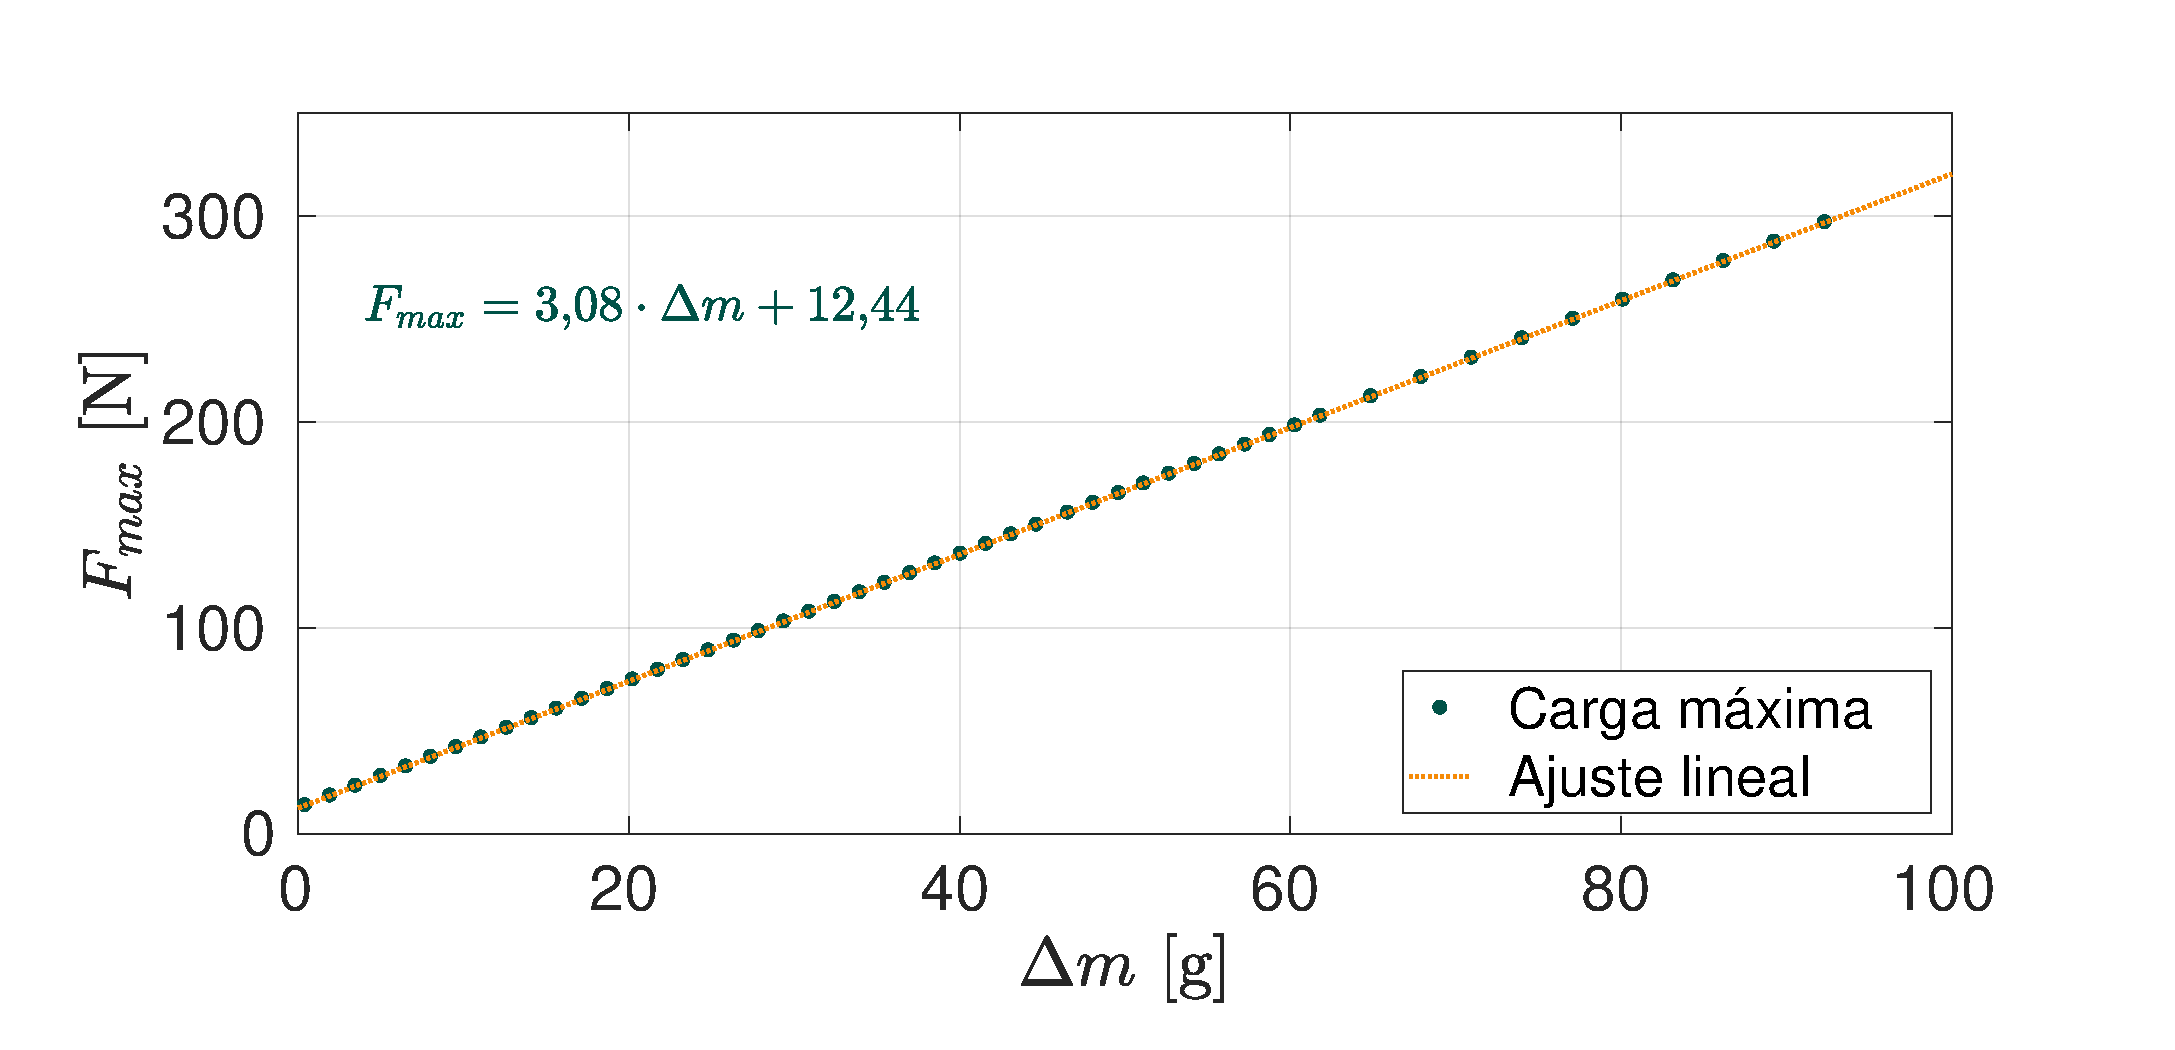
\includegraphics[width=1\linewidth, trim={1cm 0cm 2cm 0cm}, clip]{Imagenes/fmax_dmec.pdf}
\caption{Ajuste lineal de la carga máxima para las 201 combinaciones de contrapesos con $\omega_{max}=1500$ rpm.}
\label{fig:fmax_dmec}
\end{figure}
Al despejar la ecuación para $\Delta m$ se obtiene: 
\begin{equation}\label{eq:deltam}
	\Delta m = 0.325\cdot F_{max} - 4.037 \;\; [\text{g}]
\end{equation}

Por lo tanto, los contrapesos necesarios para llegar al esfuerzo de fluencia y al esfuerzo último corresponden a:
\begin{gather*}
	\Delta m_y = 142.02 \: g \\
	\Delta m_u = 320.53 \: g
\end{gather*}
Así mismo, en el anexo \ref{sec:anexob3} se encuentra la tabla con el valor $\Delta m$ para cada una de las 76 cargas aplicadas y su respectivo esfuerzo de von Mises y cortante máximo.

\subsection{Vida a fatiga para las cargas asociada a las combinaciones de contrapesos}

A partir de los esfuerzos de von Mises expuestos en el anexo \ref{sec:anexob2}, se estimará la vida a fatiga de la probeta. Se conoce el límite de resistencia a la fatiga que corresponde a $S_e = 159.013$ MPa, el esfuerzo medio $\sigma_m = 9.124$ MPa y el esfuerzo último del material $S_u = 418.5$ MPa, por lo tanto se buscará el esfuerzo alternante ($\sigma_a$) que es el punto de inflexión entre una vida finita y una infinita. 
\begin{equation}
 \sigma_a = S_e\left(1 - \frac{\sigma_m}{S_u}\right) = 149.677 \text{ MPa}
\end{equation} 

Al buscar el esfuerzo alternante más cercano obtenido por las simulaciones, se obtiene la combinación n$^{\circ}$ 173, con $\sigma_{a,173} = 148.986$ MPa. Al reemplazarlo en la ec. \ref{eq:nf_goodman} de Goodman y la ec. \ref{eq:nf_swt} de SWT, se obtiene que la vida a fatiga esperada es de $1.4\cdot 10^6$ ciclos y $1.32\cdot 10^6$ ciclos, respectivamente. Por otra parte, al utilizar la carga máxima n$^{\circ}$ 201 y reemplazar en las ecuaciones se obtiene para la relación de Goodman:
\begin{gather*}
	N_{f,g} = \frac{1}{2} \left[\frac{1}{970.45} \left(\frac{418.5\cdot 194.01}{418.5 - 9.124}\right)\right]^{-1/0.12467} \\[10pt]
	N_{f,g} = 1.69 \cdot 10^{5} ciclos
\end{gather*}
Y para la relación SWT:
\begin{gather*}
	N_{f,swt} = \frac{1}{2} \left[\frac{\sqrt{203.13\cdot 194.01}}{970.45} \right]^{-1/0.12467} \\[10pt]
	N_{f,swt} = 1.68 \cdot 10^{5} ciclos
\end{gather*}
Es decir, al utilizar el parámetro de ambas ecuaciones es posible esperar una vida a fatiga finita entre las combinaciones n$^{\circ}$ 173 y 201. Sin embargo, la fatiga al ser un fenómeno con altas fluctuaciones en sus los ensayos realizados, es posible obtener vida finita incluso a cargas menores. En la sección \ref{sec:anexob4} se encuentra la vida a fatiga esperada bajo el criterio de Goodman y SWT para las combinaciones 140 hasta 201. De manera complementaria, la fig. \ref{fig:vf_swtgd} muestra la curva de los resultados obtenidos y la tabla \ref{tab:res_vf} muestra ciertos puntos de la vida a fatiga.

\begin{table}[]
\centering
\begin{tabular}{@{}cccccc@{}}
\toprule
\begin{tabular}[c]{@{}c@{}}N$^{\circ}$ \\ Combinación\end{tabular} & $N_{f,g}$        & $N_{f,swt}$      & $\sigma_{max}$ {[}MPa{]} & $f_{a}$ {[}N{]} & $f_{max}$ {[}N{]} \\ \midrule
$201$                                                              & $1.69\cdot 10^5$ & $1.68\cdot 10^5$ & $203.13$                 & $284.476$       & $296.914$         \\
$185$                                                              & $5.27\cdot 10^5$ & $5.10\cdot 10^5$ & $177.39$                 & $246.876$       & $259.314$         \\
$176$                                                              & $1.08\cdot 10^6$ & $1.08\cdot 10^6$ & $162.94$                 & $225.761$       & $238.199$         \\
$155$                                                              & $5.74\cdot 10^6$ & $5.19\cdot 10^6$ & $133.98$                 & $183.424$       & $195.862$         \\
$142$                                                              & $1.16\cdot 10^7$ & $1.02\cdot 10^7$ & $123.5$                  & $168.114$       & $180.552$         \\
$140$                                                              & $1.30\cdot 10^7$ & $1.14\cdot 10^7$ & $121.9$                  & $165.779$       & $178.217$         \\ \bottomrule
\end{tabular}
\caption{Resultados de vida a fatiga para distintas combinaciones de contrapesos.}
\label{tab:res_vf}
\end{table}

\begin{figure}[h]
\centering
\includegraphics[width=\linewidth]{Imagenes/vidafat_swt_gd.pdf}
\caption{Curva semilogaritmica $S$-$N$ con la vida a fatiga obtenida por medio de la relación de Goodman y SWT para los esfurezos obtenidos mediante las combinaciones 140 hasta 201.}
\label{fig:vf_swtgd}
\end{figure}

%Sin embargo, no es posible dilucidar la precisión ni el error, tanto en el modelo como en la información original, debido a la imposibilidad de realizar ensayos de fatiga que nos permitan esclarecer la validez ambos métodos.

\subsection{Corroboración de la vida a fatiga y su estimación a partir de la carga alternante y media.}

A modo de corroborar la vida a fatiga obtenida, se realizarán cálculos analíticos del esfuerzo producido sobre la probeta a partir de las ecuaciones de una viga en flexión y vida a fatiga con las relaciones de Goodman y SWT.

Para esto se definirá el esfuerzo en flexión de la probeta como:
\begin{equation}
	\sigma_f = \frac{M_f \cdot c}{I} = \frac{32 f\cdot L'}{\pi \cdot d^3}
\end{equation}  

Donde $L' = 38.83$ mm corresponde a la distancia entre el lado empotrado de la probeta y la aplicación de la fuerza, $d$ el diámetro de la probeta y $f$ la fuerza que se aplicará sobre la probeta, como se muestra en la fig. \ref{fig:prob_vf}. 

\begin{figure}[h]
\centering
\includegraphics[width=0.8\linewidth, trim={-2cm -1cm -2cm 0cm}, clip]{Imagenes/probeta_carga.pdf}
\caption{Diagrama de las consideraciones utilizadas en la probeta para el cálculo del momento y el esfuerzo flector.}
\label{fig:prob_vf}
\end{figure}

De esta forma podemos definir que el esfuerzo sobre la probeta será:
\begin{equation}
	\sigma = \alpha \cdot f
\end{equation}
Donde $\alpha = 0.8939$ [1/mm$^2$]. Además, la carga media debe ser constante al realizar un ensayo de fatiga, por ende, se puede establecer una relación entre la carga alternante y la carga media que soportará la probeta:
\begin{equation} \label{eq:fa_bfm}
	f_a = \beta \cdot f_m
\end{equation}
De esta forma, se estimará la vida a fatiga de la probeta utilizando el esfuerzo equivalente proveniente de la ec. \ref{eq:sn_goodman} de Goodman normalizada ($\sigma_{eq,g}$) y la ec. \ref{eq:sn_swt} de la relación de SWT ($\sigma_{eq,swt}$) . Al escribir ambas relaciones en términos de las fuerzas se obtienen las ecuaciones \ref{eq:eq_good} y \ref{eq:eq_swt}, respectivamente:
\begin{subequations}
\begin{gather}
	\sigma_{eq,g} = \frac{\alpha \cdot \beta \cdot f_m}{\left(1 - \frac{\alpha \cdot f_m}{S_u}\right)} \label{eq:eq_good} \\[10pt]
	\sigma_{eq,swt} = \left[ \alpha^2 \cdot \beta \cdot f_m^2 (1 + \beta)\right]^{1/2} \label{eq:eq_swt}
\end{gather}
\end{subequations}

%\begin{gather}
%	\frac{\alpha \cdot \beta \cdot f_m}{\sigma_{eq}} + \frac{\alpha \cdot f_m}{S_u} = 1 \\
%	\sigma_{eq} = \frac{\alpha \cdot \beta \cdot f_m}{\left(1 - \frac{\alpha \cdot f_m}{S_u}\right)}
%\end{gather}
%
%Para la ecuación (b):
%\begin{gather}
%	\sigma_{eq} = \left[ \alpha^2 \cdot \beta \cdot f_m^2 (1 + \beta)\right]^{1/2}
%\end{gather}
 
En consecuencia, la vida a fatiga expresada en términos de la carga media y el factor $\beta$ para las relación de Goodman ($N_{f,g}$) y SWT ($N_{f,swt}$):
\begin{subequations}
\begin{gather}
	N_{f,g} = \frac{1}{2} \left[\frac{\alpha \cdot \beta \cdot f_m}{\sigma_f' \cdot \left(1 - \frac{\alpha \cdot f_m}{S_u}\right)}\right]^{1/b} \\[10pt]
	N_{f,swt} = \frac{1}{2}\left[\frac{\left[ \alpha^2 \cdot \beta \cdot f_m^2 (1 + \beta)\right]^{1/2}}{\sigma_f'}\right]^{1/b}
\end{gather}
\end{subequations}

Así, ambas ecuaciones se pueden resolver para distintos valores de vida a fatiga en conjunto a la ec. \ref{eq:fa_bfm}. Los valores de las distintas constantes son:
\begin{multicols}{2}
\begin{itemize*}
	\item $\alpha = 0.8939\:$ [1/mm$^2$]
	\item $f_m = 12.438\:$ [N]
	\item $\sigma'_f = 970.45\:$ [MPa]
	\item $S_u = 418.5\:$ [MPa]
	\item $b = -0.12467\:$ [-]
\end{itemize*}
\end{multicols}

Finalmente, al reemplazar y resolver ambas ecuaciones, se obtienen los resultados expuestos en la tabla \ref{tab:resfuerza_vf}.

\begin{table}[h]
\centering
\begin{tabular}{@{}ccccccc@{}}
\toprule
       & \multicolumn{3}{c}{Goodman}                  & \multicolumn{3}{c}{SWT}                      \\ \cmidrule(l){2-7} 
$N_f$  & $\beta$  & $f_a$ {[}N{]} & $f_{max}$ {[}N{]} & $\beta$  & $f_a$ {[}N{]} & $f_{max}$ {[}N{]} \\ \midrule
$10^4$ & $24.719$ & $307.454$     & $319.892$         & $24.898$ & $309.688$     & $322.126$         \\
$10^5$ & $18.550$ & $230.733$     & $243.171$         & $18.563$ & $230.893$     & $243.331$         \\
$10^6$ & $13.922$ & $173.157$     & $185.595$         & $13.810$ & $171.773$     & $184.210$         \\
$10^7$ & $10.447$ & $129.948$     & $142.386$         & $10.244$ & $127.421$     & $139.859$         \\ \bottomrule
\end{tabular}
\caption{Fuerza alternante, máxima y el coeficiente $\beta$ obtenido para distintos valores de vida a fatiga para la relación de Goodman y SWT.}
\label{tab:resfuerza_vf}
\end{table}

Al comparar los resultados de las tablas \ref{tab:res_vf} y \ref{tab:resfuerza_vf} se aprecia que existe una diferencia entre ambos resultados, sin embargo, el orden de magnitud de los resultados es cercano y nos permite corroborar los datos mostrados en la tabla \ref{sec:anexob4}. Por otro lado, al comparar los resultados de los métodos utilizados de Goodman y SWT, estos son bastante cercanos en sus límites de aplicación, es decir, entre $10^4$ y $10^7$ ciclos. A pesar de que la relación SWT es más conservadora que la relación de Goodman, la elección de uno por sobre otro no afecta considerablemente la vida a fatiga esperable al encontrarse ambos métodos siempre en el mismo orden de magnitud. Finalmente, es necesario realizar una validación experimental que permita contrastar estos resultados y, de esta manera, conocer el error de la metodología utilizada, como también lograr identificar aquellos elementos que permitan realizar predicciones más precisas.

